\documentclass{report}

%%%%%%%%%%%%%%%%%%%%%%%%%%%%%%%%%
% PACKAGE IMPORTS
%%%%%%%%%%%%%%%%%%%%%%%%%%%%%%%%%
\usepackage[tmargin=2cm,rmargin=1in,lmargin=1in,margin=0.85in,bmargin=2cm,footskip=.2in]{geometry}
\usepackage{amsmath,amsfonts,amsthm,amssymb,mathtools}
\usepackage[varbb]{newpxmath}
\usepackage{xfrac}
\usepackage[makeroom]{cancel}
\usepackage{mathtools}
\usepackage{bookmark}
\usepackage{enumitem}
\usepackage{hyperref,theoremref}
\hypersetup{
	pdftitle={Assignment},
	colorlinks=true, linkcolor=doc!90,
	bookmarksnumbered=true,
	bookmarksopen=true
}
\usepackage[most,many,breakable]{tcolorbox}
\usepackage{xcolor}
\usepackage{varwidth}
\usepackage{varwidth}
\usepackage{etoolbox}
%\usepackage{authblk}
\usepackage{nameref}
\usepackage{multicol,array}
\usepackage[ruled,vlined,linesnumbered]{algorithm2e}
\usepackage{comment} % enables the use of multi-line comments (\ifx \fi) 
\usepackage{import}
\usepackage{xifthen}
\usepackage{pdfpages}
\usepackage{transparent}

\newcommand\mycommfont[1]{\footnotesize\ttfamily\textcolor{blue}{#1}}
\SetCommentSty{mycommfont}
\newcommand{\incfig}[1]{%
    \def\svgwidth{\columnwidth}
    \import{./figures/}{#1.pdf_tex}
}

\usepackage{tikzsymbols}
\renewcommand\qedsymbol{$\Laughey$}


%\usepackage{import}
%\usepackage{xifthen}
%\usepackage{pdfpages}
%\usepackage{transparent}


%%%%%%%%%%%%%%%%%%%%%%%%%%%%%%
% SELF MADE COLORS
%%%%%%%%%%%%%%%%%%%%%%%%%%%%%%



\definecolor{myg}{RGB}{56, 140, 70}
\definecolor{myb}{RGB}{45, 111, 177}
\definecolor{myr}{RGB}{199, 68, 64}
\definecolor{mytheorembg}{HTML}{F2F2F9}
\definecolor{mytheoremfr}{HTML}{00007B}
\definecolor{mylenmabg}{HTML}{FFFAF8}
\definecolor{mylenmafr}{HTML}{983b0f}
\definecolor{mypropbg}{HTML}{f2fbfc}
\definecolor{mypropfr}{HTML}{191971}
\definecolor{myexamplebg}{HTML}{F2FBF8}
\definecolor{myexamplefr}{HTML}{88D6D1}
\definecolor{myexampleti}{HTML}{2A7F7F}
\definecolor{mydefinitbg}{HTML}{E5E5FF}
\definecolor{mydefinitfr}{HTML}{3F3FA3}
\definecolor{notesgreen}{RGB}{0,162,0}
\definecolor{myp}{RGB}{197, 92, 212}
\definecolor{mygr}{HTML}{2C3338}
\definecolor{myred}{RGB}{127,0,0}
\definecolor{myyellow}{RGB}{169,121,69}
\definecolor{myexercisebg}{HTML}{F2FBF8}
\definecolor{myexercisefg}{HTML}{88D6D1}



%%%%%%%%%%%%%%%%%%%%%%%%%%%%
% TCOLORBOX SETUPS
%%%%%%%%%%%%%%%%%%%%%%%%%%%%

\setlength{\parindent}{1cm}
%================================
% THEOREM BOX
%================================

\tcbuselibrary{theorems,skins,hooks}
\newtcbtheorem[number within=section]{Theorem}{Theorem}
{%
	enhanced,
	breakable,
	colback = mytheorembg,
	frame hidden,
	boxrule = 0sp,
	borderline west = {2pt}{0pt}{mytheoremfr},
	sharp corners,
	detach title,
	before upper = \tcbtitle\par\smallskip,
	coltitle = mytheoremfr,
	fonttitle = \bfseries\sffamily,
	description font = \mdseries,
	separator sign none,
	segmentation style={solid, mytheoremfr},
}
{th}

\tcbuselibrary{theorems,skins,hooks}
\newtcbtheorem[number within=chapter]{theorem}{Theorem}
{%
	enhanced,
	breakable,
	colback = mytheorembg,
	frame hidden,
	boxrule = 0sp,
	borderline west = {2pt}{0pt}{mytheoremfr},
	sharp corners,
	detach title,
	before upper = \tcbtitle\par\smallskip,
	coltitle = mytheoremfr,
	fonttitle = \bfseries\sffamily,
	description font = \mdseries,
	separator sign none,
	segmentation style={solid, mytheoremfr},
}
{th}


\tcbuselibrary{theorems,skins,hooks}
\newtcolorbox{Theoremcon}
{%
	enhanced
	,breakable
	,colback = mytheorembg
	,frame hidden
	,boxrule = 0sp
	,borderline west = {2pt}{0pt}{mytheoremfr}
	,sharp corners
	,description font = \mdseries
	,separator sign none
}

%================================
% Corollery
%================================
\tcbuselibrary{theorems,skins,hooks}
\newtcbtheorem[number within=section]{Corollary}{Corollary}
{%
	enhanced
	,breakable
	,colback = myp!10
	,frame hidden
	,boxrule = 0sp
	,borderline west = {2pt}{0pt}{myp!85!black}
	,sharp corners
	,detach title
	,before upper = \tcbtitle\par\smallskip
	,coltitle = myp!85!black
	,fonttitle = \bfseries\sffamily
	,description font = \mdseries
	,separator sign none
	,segmentation style={solid, myp!85!black}
}
{th}
\tcbuselibrary{theorems,skins,hooks}
\newtcbtheorem[number within=chapter]{corollary}{Corollary}
{%
	enhanced
	,breakable
	,colback = myp!10
	,frame hidden
	,boxrule = 0sp
	,borderline west = {2pt}{0pt}{myp!85!black}
	,sharp corners
	,detach title
	,before upper = \tcbtitle\par\smallskip
	,coltitle = myp!85!black
	,fonttitle = \bfseries\sffamily
	,description font = \mdseries
	,separator sign none
	,segmentation style={solid, myp!85!black}
}
{th}


%================================
% LENMA
%================================

\tcbuselibrary{theorems,skins,hooks}
\newtcbtheorem[number within=section]{Lenma}{Lenma}
{%
	enhanced,
	breakable,
	colback = mylenmabg,
	frame hidden,
	boxrule = 0sp,
	borderline west = {2pt}{0pt}{mylenmafr},
	sharp corners,
	detach title,
	before upper = \tcbtitle\par\smallskip,
	coltitle = mylenmafr,
	fonttitle = \bfseries\sffamily,
	description font = \mdseries,
	separator sign none,
	segmentation style={solid, mylenmafr},
}
{th}

\tcbuselibrary{theorems,skins,hooks}
\newtcbtheorem[number within=chapter]{lenma}{Lenma}
{%
	enhanced,
	breakable,
	colback = mylenmabg,
	frame hidden,
	boxrule = 0sp,
	borderline west = {2pt}{0pt}{mylenmafr},
	sharp corners,
	detach title,
	before upper = \tcbtitle\par\smallskip,
	coltitle = mylenmafr,
	fonttitle = \bfseries\sffamily,
	description font = \mdseries,
	separator sign none,
	segmentation style={solid, mylenmafr},
}
{th}

%================================
% Exercise
%================================

\tcbuselibrary{theorems,skins,hooks}
\newtcbtheorem[number within=section]{Exercise}{Exercise}
{%
	enhanced,
	breakable,
	colback = myexercisebg,
	frame hidden,
	boxrule = 0sp,
	borderline west = {2pt}{0pt}{myexercisefg},
	sharp corners,
	detach title,
	before upper = \tcbtitle\par\smallskip,
	coltitle = myexercisefg,
	fonttitle = \bfseries\sffamily,
	description font = \mdseries,
	separator sign none,
	segmentation style={solid, myexercisefg},
}
{th}

\tcbuselibrary{theorems,skins,hooks}
\newtcbtheorem[number within=chapter]{exercise}{Exercise}
{%
	enhanced,
	breakable,
	colback = myexercisebg,
	frame hidden,
	boxrule = 0sp,
	borderline west = {2pt}{0pt}{myexercisefg},
	sharp corners,
	detach title,
	before upper = \tcbtitle\par\smallskip,
	coltitle = myexercisefg,
	fonttitle = \bfseries\sffamily,
	description font = \mdseries,
	separator sign none,
	segmentation style={solid, myexercisefg},
}
{th}



%================================
% PROPOSITION
%================================

\tcbuselibrary{theorems,skins,hooks}
\newtcbtheorem[number within=section]{Prop}{Proposition}
{%
	enhanced,
	breakable,
	colback = mypropbg,
	frame hidden,
	boxrule = 0sp,
	borderline west = {2pt}{0pt}{mypropfr},
	sharp corners,
	detach title,
	before upper = \tcbtitle\par\smallskip,
	coltitle = mypropfr,
	fonttitle = \bfseries\sffamily,
	description font = \mdseries,
	separator sign none,
	segmentation style={solid, mypropfr},
}
{th}

\tcbuselibrary{theorems,skins,hooks}
\newtcbtheorem[number within=chapter]{prop}{Proposition}
{%
	enhanced,
	breakable,
	colback = mypropbg,
	frame hidden,
	boxrule = 0sp,
	borderline west = {2pt}{0pt}{mypropfr},
	sharp corners,
	detach title,
	before upper = \tcbtitle\par\smallskip,
	coltitle = mypropfr,
	fonttitle = \bfseries\sffamily,
	description font = \mdseries,
	separator sign none,
	segmentation style={solid, mypropfr},
}
{th}


%================================
% CLAIM
%================================

\tcbuselibrary{theorems,skins,hooks}
\newtcbtheorem[number within=section]{claim}{Claim}
{%
	enhanced
	,breakable
	,colback = myg!10
	,frame hidden
	,boxrule = 0sp
	,borderline west = {2pt}{0pt}{myg}
	,sharp corners
	,detach title
	,before upper = \tcbtitle\par\smallskip
	,coltitle = myg!85!black
	,fonttitle = \bfseries\sffamily
	,description font = \mdseries
	,separator sign none
	,segmentation style={solid, myg!85!black}
}
{th}




%================================
% EXAMPLE BOX
%================================

\newtcbtheorem[number within=section]{Example}{Example}
{%
	colback = myexamplebg
	,breakable
	,colframe = myexamplefr
	,coltitle = myexampleti
	,boxrule = 1pt
	,sharp corners
	,detach title
	,before upper=\tcbtitle\par\smallskip
	,fonttitle = \bfseries
	,description font = \mdseries
	,separator sign none
	,description delimiters parenthesis
}
{ex}

\newtcbtheorem[number within=chapter]{example}{Example}
{%
	colback = myexamplebg
	,breakable
	,colframe = myexamplefr
	,coltitle = myexampleti
	,boxrule = 1pt
	,sharp corners
	,detach title
	,before upper=\tcbtitle\par\smallskip
	,fonttitle = \bfseries
	,description font = \mdseries
	,separator sign none
	,description delimiters parenthesis
}
{ex}

%================================
% DEFINITION BOX
%================================

\newtcbtheorem[number within=section]{Definition}{Definition}{enhanced,
	before skip=2mm,after skip=2mm, colback=red!5,colframe=red!80!black,boxrule=0.5mm,
	attach boxed title to top left={xshift=1cm,yshift*=1mm-\tcboxedtitleheight}, varwidth boxed title*=-3cm,
	boxed title style={frame code={
					\path[fill=tcbcolback]
					([yshift=-1mm,xshift=-1mm]frame.north west)
					arc[start angle=0,end angle=180,radius=1mm]
					([yshift=-1mm,xshift=1mm]frame.north east)
					arc[start angle=180,end angle=0,radius=1mm];
					\path[left color=tcbcolback!60!black,right color=tcbcolback!60!black,
						middle color=tcbcolback!80!black]
					([xshift=-2mm]frame.north west) -- ([xshift=2mm]frame.north east)
					[rounded corners=1mm]-- ([xshift=1mm,yshift=-1mm]frame.north east)
					-- (frame.south east) -- (frame.south west)
					-- ([xshift=-1mm,yshift=-1mm]frame.north west)
					[sharp corners]-- cycle;
				},interior engine=empty,
		},
	fonttitle=\bfseries,
	title={#2},#1}{def}
\newtcbtheorem[number within=chapter]{definition}{Definition}{enhanced,
	before skip=2mm,after skip=2mm, colback=red!5,colframe=red!80!black,boxrule=0.5mm,
	attach boxed title to top left={xshift=1cm,yshift*=1mm-\tcboxedtitleheight}, varwidth boxed title*=-3cm,
	boxed title style={frame code={
					\path[fill=tcbcolback]
					([yshift=-1mm,xshift=-1mm]frame.north west)
					arc[start angle=0,end angle=180,radius=1mm]
					([yshift=-1mm,xshift=1mm]frame.north east)
					arc[start angle=180,end angle=0,radius=1mm];
					\path[left color=tcbcolback!60!black,right color=tcbcolback!60!black,
						middle color=tcbcolback!80!black]
					([xshift=-2mm]frame.north west) -- ([xshift=2mm]frame.north east)
					[rounded corners=1mm]-- ([xshift=1mm,yshift=-1mm]frame.north east)
					-- (frame.south east) -- (frame.south west)
					-- ([xshift=-1mm,yshift=-1mm]frame.north west)
					[sharp corners]-- cycle;
				},interior engine=empty,
		},
	fonttitle=\bfseries,
	title={#2},#1}{def}



%================================
% EXERCISE BOX
%================================

\makeatletter
\newtcbtheorem{question}{Question}{enhanced,
	breakable,
	colback=white,
	colframe=myb!80!black,
	attach boxed title to top left={yshift*=-\tcboxedtitleheight},
	fonttitle=\bfseries,
	title={#2},
	boxed title size=title,
	boxed title style={%
			sharp corners,
			rounded corners=northwest,
			colback=tcbcolframe,
			boxrule=0pt,
		},
	underlay boxed title={%
			\path[fill=tcbcolframe] (title.south west)--(title.south east)
			to[out=0, in=180] ([xshift=5mm]title.east)--
			(title.center-|frame.east)
			[rounded corners=\kvtcb@arc] |-
			(frame.north) -| cycle;
		},
	#1
}{def}
\makeatother

%================================
% SOLUTION BOX
%================================

\makeatletter
\newtcolorbox{solution}{enhanced,
	breakable,
	colback=white,
	colframe=myg!80!black,
	attach boxed title to top left={yshift*=-\tcboxedtitleheight},
	title=Solution,
	boxed title size=title,
	boxed title style={%
			sharp corners,
			rounded corners=northwest,
			colback=tcbcolframe,
			boxrule=0pt,
		},
	underlay boxed title={%
			\path[fill=tcbcolframe] (title.south west)--(title.south east)
			to[out=0, in=180] ([xshift=5mm]title.east)--
			(title.center-|frame.east)
			[rounded corners=\kvtcb@arc] |-
			(frame.north) -| cycle;
		},
}
\makeatother

%================================
% Question BOX
%================================

\makeatletter
\newtcbtheorem{qstion}{Question}{enhanced,
	breakable,
	colback=white,
	colframe=mygr,
	attach boxed title to top left={yshift*=-\tcboxedtitleheight},
	fonttitle=\bfseries,
	title={#2},
	boxed title size=title,
	boxed title style={%
			sharp corners,
			rounded corners=northwest,
			colback=tcbcolframe,
			boxrule=0pt,
		},
	underlay boxed title={%
			\path[fill=tcbcolframe] (title.south west)--(title.south east)
			to[out=0, in=180] ([xshift=5mm]title.east)--
			(title.center-|frame.east)
			[rounded corners=\kvtcb@arc] |-
			(frame.north) -| cycle;
		},
	#1
}{def}
\makeatother

\newtcbtheorem[number within=chapter]{wconc}{Wrong Concept}{
	breakable,
	enhanced,
	colback=white,
	colframe=myr,
	arc=0pt,
	outer arc=0pt,
	fonttitle=\bfseries\sffamily\large,
	colbacktitle=myr,
	attach boxed title to top left={},
	boxed title style={
			enhanced,
			skin=enhancedfirst jigsaw,
			arc=3pt,
			bottom=0pt,
			interior style={fill=myr}
		},
	#1
}{def}



%================================
% NOTE BOX
%================================

\usetikzlibrary{arrows,calc,shadows.blur}
\tcbuselibrary{skins}
\newtcolorbox{note}[1][]{%
	enhanced jigsaw,
	colback=gray!20!white,%
	colframe=gray!80!black,
	size=small,
	boxrule=1pt,
	title=\textbf{Note:-},
	halign title=flush center,
	coltitle=black,
	breakable,
	drop shadow=black!50!white,
	attach boxed title to top left={xshift=1cm,yshift=-\tcboxedtitleheight/2,yshifttext=-\tcboxedtitleheight/2},
	minipage boxed title=1.5cm,
	boxed title style={%
			colback=white,
			size=fbox,
			boxrule=1pt,
			boxsep=2pt,
			underlay={%
					\coordinate (dotA) at ($(interior.west) + (-0.5pt,0)$);
					\coordinate (dotB) at ($(interior.east) + (0.5pt,0)$);
					\begin{scope}
						\clip (interior.north west) rectangle ([xshift=3ex]interior.east);
						\filldraw [white, blur shadow={shadow opacity=60, shadow yshift=-.75ex}, rounded corners=2pt] (interior.north west) rectangle (interior.south east);
					\end{scope}
					\begin{scope}[gray!80!black]
						\fill (dotA) circle (2pt);
						\fill (dotB) circle (2pt);
					\end{scope}
				},
		},
	#1,
}

%%%%%%%%%%%%%%%%%%%%%%%%%%%%%%
% SELF MADE COMMANDS
%%%%%%%%%%%%%%%%%%%%%%%%%%%%%%


\newcommand{\thm}[2]{\begin{Theorem}{#1}{}#2\end{Theorem}}
\newcommand{\cor}[2]{\begin{Corollary}{#1}{}#2\end{Corollary}}
\newcommand{\mlenma}[2]{\begin{Lenma}{#1}{}#2\end{Lenma}}
\newcommand{\mer}[2]{\begin{Exercise}{#1}{}#2\end{Exercise}}
\newcommand{\mprop}[2]{\begin{Prop}{#1}{}#2\end{Prop}}
\newcommand{\clm}[3]{\begin{claim}{#1}{#2}#3\end{claim}}
\newcommand{\wc}[2]{\begin{wconc}{#1}{}\setlength{\parindent}{1cm}#2\end{wconc}}
\newcommand{\thmcon}[1]{\begin{Theoremcon}{#1}\end{Theoremcon}}
\newcommand{\ex}[2]{\begin{Example}{#1}{}#2\end{Example}}
\newcommand{\dfn}[2]{\begin{Definition}[colbacktitle=red!75!black]{#1}{}#2\end{Definition}}
\newcommand{\dfnc}[2]{\begin{definition}[colbacktitle=red!75!black]{#1}{}#2\end{definition}}
\newcommand{\qs}[2]{\begin{question}{#1}{}#2\end{question}}
\newcommand{\pf}[2]{\begin{myproof}[#1]#2\end{myproof}}
\newcommand{\nt}[1]{\begin{note}#1\end{note}}

\newcommand*\circled[1]{\tikz[baseline=(char.base)]{
		\node[shape=circle,draw,inner sep=1pt] (char) {#1};}}
\newcommand\getcurrentref[1]{%
	\ifnumequal{\value{#1}}{0}
	{??}
	{\the\value{#1}}%
}
\newcommand{\getCurrentSectionNumber}{\getcurrentref{section}}
\newenvironment{myproof}[1][\proofname]{%
	\proof[\bfseries #1: ]%
}{\endproof}

\newcommand{\mclm}[2]{\begin{myclaim}[#1]#2\end{myclaim}}
\newenvironment{myclaim}[1][\claimname]{\proof[\bfseries #1: ]}{}

\newcounter{mylabelcounter}

\makeatletter
\newcommand{\setword}[2]{%
	\phantomsection
	#1\def\@currentlabel{\unexpanded{#1}}\label{#2}%
}
\makeatother




\tikzset{
	symbol/.style={
			draw=none,
			every to/.append style={
					edge node={node [sloped, allow upside down, auto=false]{$#1$}}}
		}
}


% deliminators
\DeclarePairedDelimiter{\abs}{\lvert}{\rvert}
\DeclarePairedDelimiter{\norm}{\lVert}{\rVert}

\DeclarePairedDelimiter{\ceil}{\lceil}{\rceil}
\DeclarePairedDelimiter{\floor}{\lfloor}{\rfloor}
\DeclarePairedDelimiter{\round}{\lfloor}{\rceil}

\newsavebox\diffdbox
\newcommand{\slantedromand}{{\mathpalette\makesl{d}}}
\newcommand{\makesl}[2]{%
\begingroup
\sbox{\diffdbox}{$\mathsurround=0pt#1\mathrm{#2}$}%
\pdfsave
\pdfsetmatrix{1 0 0.2 1}%
\rlap{\usebox{\diffdbox}}%
\pdfrestore
\hskip\wd\diffdbox
\endgroup
}
\newcommand{\dd}[1][]{\ensuremath{\mathop{}\!\ifstrempty{#1}{%
\slantedromand\@ifnextchar^{\hspace{0.2ex}}{\hspace{0.1ex}}}%
{\slantedromand\hspace{0.2ex}^{#1}}}}
\ProvideDocumentCommand\dv{o m g}{%
  \ensuremath{%
    \IfValueTF{#3}{%
      \IfNoValueTF{#1}{%
        \frac{\dd #2}{\dd #3}%
      }{%
        \frac{\dd^{#1} #2}{\dd #3^{#1}}%
      }%
    }{%
      \IfNoValueTF{#1}{%
        \frac{\dd}{\dd #2}%
      }{%
        \frac{\dd^{#1}}{\dd #2^{#1}}%
      }%
    }%
  }%
}
\providecommand*{\pdv}[3][]{\frac{\partial^{#1}#2}{\partial#3^{#1}}}
%  - others
\DeclareMathOperator{\Lap}{\mathcal{L}}
\DeclareMathOperator{\Var}{Var} % varience
\DeclareMathOperator{\Cov}{Cov} % covarience
\DeclareMathOperator{\E}{E} % expected

% Since the amsthm package isn't loaded

% I prefer the slanted \leq
\let\oldleq\leq % save them in case they're every wanted
\let\oldgeq\geq
\renewcommand{\leq}{\leqslant}
\renewcommand{\geq}{\geqslant}

% % redefine matrix env to allow for alignment, use r as default
% \renewcommand*\env@matrix[1][r]{\hskip -\arraycolsep
%     \let\@ifnextchar\new@ifnextchar
%     \array{*\c@MaxMatrixCols #1}}


%\usepackage{framed}
%\usepackage{titletoc}
%\usepackage{etoolbox}
%\usepackage{lmodern}


%\patchcmd{\tableofcontents}{\contentsname}{\sffamily\contentsname}{}{}

%\renewenvironment{leftbar}
%{\def\FrameCommand{\hspace{6em}%
%		{\color{myyellow}\vrule width 2pt depth 6pt}\hspace{1em}}%
%	\MakeFramed{\parshape 1 0cm \dimexpr\textwidth-6em\relax\FrameRestore}\vskip2pt%
%}
%{\endMakeFramed}

%\titlecontents{chapter}
%[0em]{\vspace*{2\baselineskip}}
%{\parbox{4.5em}{%
%		\hfill\Huge\sffamily\bfseries\color{myred}\thecontentspage}%
%	\vspace*{-2.3\baselineskip}\leftbar\textsc{\small\chaptername~\thecontentslabel}\\\sffamily}
%{}{\endleftbar}
%\titlecontents{section}
%[8.4em]
%{\sffamily\contentslabel{3em}}{}{}
%{\hspace{0.5em}\nobreak\itshape\color{myred}\contentspage}
%\titlecontents{subsection}
%[8.4em]
%{\sffamily\contentslabel{3em}}{}{}  
%{\hspace{0.5em}\nobreak\itshape\color{myred}\contentspage}



%%%%%%%%%%%%%%%%%%%%%%%%%%%%%%%%%%%%%%%%%%%
% TABLE OF CONTENTS
%%%%%%%%%%%%%%%%%%%%%%%%%%%%%%%%%%%%%%%%%%%

\usepackage{tikz}
\definecolor{doc}{RGB}{0,60,110}
\usepackage{titletoc}
\contentsmargin{0cm}
\titlecontents{chapter}[3.7pc]
{\addvspace{30pt}%
	\begin{tikzpicture}[remember picture, overlay]%
		\draw[fill=doc!60,draw=doc!60] (-7,-.1) rectangle (-0.9,.5);%
		\pgftext[left,x=-3.7cm,y=0.2cm]{\color{white}\Large\sc\bfseries Chapter\ \thecontentslabel};%
	\end{tikzpicture}\color{doc!60}\large\sc\bfseries}%
{}
{}
{\;\titlerule\;\large\sc\bfseries Page \thecontentspage
	\begin{tikzpicture}[remember picture, overlay]
		\draw[fill=doc!60,draw=doc!60] (2pt,0) rectangle (4,0.1pt);
	\end{tikzpicture}}%
\titlecontents{section}[3.7pc]
{\addvspace{2pt}}
{\contentslabel[\thecontentslabel]{2pc}}
{}
{\hfill\small \thecontentspage}
[]
\titlecontents*{subsection}[3.7pc]
{\addvspace{-1pt}\small}
{}
{}
{\ --- \small\thecontentspage}
[ \textbullet\ ][]

\makeatletter
\renewcommand{\tableofcontents}{%
	\chapter*{%
	  \vspace*{-20\p@}%
	  \begin{tikzpicture}[remember picture, overlay]%
		  \pgftext[right,x=15cm,y=0.2cm]{\color{doc!60}\Huge\sc\bfseries \contentsname};%
		  \draw[fill=doc!60,draw=doc!60] (13,-.75) rectangle (20,1);%
		  \clip (13,-.75) rectangle (20,1);
		  \pgftext[right,x=15cm,y=0.2cm]{\color{white}\Huge\sc\bfseries \contentsname};%
	  \end{tikzpicture}}%
	\@starttoc{toc}}
\makeatother


\newcommand{\eps}{\epsilon}
\newcommand{\veps}{\varepsilon}
\newcommand{\Qed}{\begin{flushright}\qed\end{flushright}}

\newcommand{\parinn}{\setlength{\parindent}{1cm}}
\newcommand{\parinf}{\setlength{\parindent}{0cm}}

% \newcommand{\norm}{\|\cdot\|}
\newcommand{\inorm}{\norm_{\infty}}
\newcommand{\opensets}{\{V_{\alpha}\}_{\alpha\in I}}
\newcommand{\oset}{V_{\alpha}}
\newcommand{\opset}[1]{V_{\alpha_{#1}}}
\newcommand{\lub}{\text{lub}}
\newcommand{\del}[2]{\frac{\partial #1}{\partial #2}}
\newcommand{\Del}[3]{\frac{\partial^{#1} #2}{\partial^{#1} #3}}
\newcommand{\deld}[2]{\dfrac{\partial #1}{\partial #2}}
\newcommand{\Deld}[3]{\dfrac{\partial^{#1} #2}{\partial^{#1} #3}}
\newcommand{\lm}{\lambda}
\newcommand{\uin}{\mathbin{\rotatebox[origin=c]{90}{$\in$}}}
\newcommand{\usubset}{\mathbin{\rotatebox[origin=c]{90}{$\subset$}}}
\newcommand{\lt}{\left}
\newcommand{\rt}{\right}
\newcommand{\bs}[1]{\boldsymbol{#1}}
\newcommand{\exs}{\exists}
\newcommand{\st}{\strut}
\newcommand{\dps}[1]{\displaystyle{#1}}

\newcommand{\sol}{\setlength{\parindent}{0cm}\textbf{\textit{Solution:}}\setlength{\parindent}{1cm} }
\newcommand{\solve}[1]{\setlength{\parindent}{0cm}\textbf{\textit{Solution: }}\setlength{\parindent}{1cm}#1 \Qed}

% number sets
\newcommand{\RR}[1][]{\ensuremath{\ifstrempty{#1}{\mathbb{R}}{\mathbb{R}^{#1}}}}
\newcommand{\NN}[1][]{\ensuremath{\ifstrempty{#1}{\mathbb{N}}{\mathbb{N}^{#1}}}}
\newcommand{\ZZ}[1][]{\ensuremath{\ifstrempty{#1}{\mathbb{Z}}{\mathbb{Z}^{#1}}}}
\newcommand{\QQ}[1][]{\ensuremath{\ifstrempty{#1}{\mathbb{Q}}{\mathbb{Q}^{#1}}}}
\newcommand{\CC}[1][]{\ensuremath{\ifstrempty{#1}{\mathbb{C}}{\mathbb{C}^{#1}}}}
\newcommand{\PP}[1][]{\ensuremath{\ifstrempty{#1}{\mathbb{P}}{\mathbb{P}^{#1}}}}
\newcommand{\HH}[1][]{\ensuremath{\ifstrempty{#1}{\mathbb{H}}{\mathbb{H}^{#1}}}}
\newcommand{\FF}[1][]{\ensuremath{\ifstrempty{#1}{\mathbb{F}}{\mathbb{F}^{#1}}}}
% expected value
\newcommand{\EE}{\ensuremath{\mathbb{E}}}

%---------------------------------------
% BlackBoard Math Fonts :-
%---------------------------------------

%Captital Letters
\newcommand{\bbA}{\mathbb{A}}	\newcommand{\bbB}{\mathbb{B}}
\newcommand{\bbC}{\mathbb{C}}	\newcommand{\bbD}{\mathbb{D}}
\newcommand{\bbE}{\mathbb{E}}	\newcommand{\bbF}{\mathbb{F}}
\newcommand{\bbG}{\mathbb{G}}	\newcommand{\bbH}{\mathbb{H}}
\newcommand{\bbI}{\mathbb{I}}	\newcommand{\bbJ}{\mathbb{J}}
\newcommand{\bbK}{\mathbb{K}}	\newcommand{\bbL}{\mathbb{L}}
\newcommand{\bbM}{\mathbb{M}}	\newcommand{\bbN}{\mathbb{N}}
\newcommand{\bbO}{\mathbb{O}}	\newcommand{\bbP}{\mathbb{P}}
\newcommand{\bbQ}{\mathbb{Q}}	\newcommand{\bbR}{\mathbb{R}}
\newcommand{\bbS}{\mathbb{S}}	\newcommand{\bbT}{\mathbb{T}}
\newcommand{\bbU}{\mathbb{U}}	\newcommand{\bbV}{\mathbb{V}}
\newcommand{\bbW}{\mathbb{W}}	\newcommand{\bbX}{\mathbb{X}}
\newcommand{\bbY}{\mathbb{Y}}	\newcommand{\bbZ}{\mathbb{Z}}

%---------------------------------------
% MathCal Fonts :-
%---------------------------------------

%Captital Letters
\newcommand{\mcA}{\mathcal{A}}	\newcommand{\mcB}{\mathcal{B}}
\newcommand{\mcC}{\mathcal{C}}	\newcommand{\mcD}{\mathcal{D}}
\newcommand{\mcE}{\mathcal{E}}	\newcommand{\mcF}{\mathcal{F}}
\newcommand{\mcG}{\mathcal{G}}	\newcommand{\mcH}{\mathcal{H}}
\newcommand{\mcI}{\mathcal{I}}	\newcommand{\mcJ}{\mathcal{J}}
\newcommand{\mcK}{\mathcal{K}}	\newcommand{\mcL}{\mathcal{L}}
\newcommand{\mcM}{\mathcal{M}}	\newcommand{\mcN}{\mathcal{N}}
\newcommand{\mcO}{\mathcal{O}}	\newcommand{\mcP}{\mathcal{P}}
\newcommand{\mcQ}{\mathcal{Q}}	\newcommand{\mcR}{\mathcal{R}}
\newcommand{\mcS}{\mathcal{S}}	\newcommand{\mcT}{\mathcal{T}}
\newcommand{\mcU}{\mathcal{U}}	\newcommand{\mcV}{\mathcal{V}}
\newcommand{\mcW}{\mathcal{W}}	\newcommand{\mcX}{\mathcal{X}}
\newcommand{\mcY}{\mathcal{Y}}	\newcommand{\mcZ}{\mathcal{Z}}



%---------------------------------------
% Bold Math Fonts :-
%---------------------------------------

%Captital Letters
\newcommand{\bmA}{\boldsymbol{A}}	\newcommand{\bmB}{\boldsymbol{B}}
\newcommand{\bmC}{\boldsymbol{C}}	\newcommand{\bmD}{\boldsymbol{D}}
\newcommand{\bmE}{\boldsymbol{E}}	\newcommand{\bmF}{\boldsymbol{F}}
\newcommand{\bmG}{\boldsymbol{G}}	\newcommand{\bmH}{\boldsymbol{H}}
\newcommand{\bmI}{\boldsymbol{I}}	\newcommand{\bmJ}{\boldsymbol{J}}
\newcommand{\bmK}{\boldsymbol{K}}	\newcommand{\bmL}{\boldsymbol{L}}
\newcommand{\bmM}{\boldsymbol{M}}	\newcommand{\bmN}{\boldsymbol{N}}
\newcommand{\bmO}{\boldsymbol{O}}	\newcommand{\bmP}{\boldsymbol{P}}
\newcommand{\bmQ}{\boldsymbol{Q}}	\newcommand{\bmR}{\boldsymbol{R}}
\newcommand{\bmS}{\boldsymbol{S}}	\newcommand{\bmT}{\boldsymbol{T}}
\newcommand{\bmU}{\boldsymbol{U}}	\newcommand{\bmV}{\boldsymbol{V}}
\newcommand{\bmW}{\boldsymbol{W}}	\newcommand{\bmX}{\boldsymbol{X}}
\newcommand{\bmY}{\boldsymbol{Y}}	\newcommand{\bmZ}{\boldsymbol{Z}}
%Small Letters
\newcommand{\bma}{\boldsymbol{a}}	\newcommand{\bmb}{\boldsymbol{b}}
\newcommand{\bmc}{\boldsymbol{c}}	\newcommand{\bmd}{\boldsymbol{d}}
\newcommand{\bme}{\boldsymbol{e}}	\newcommand{\bmf}{\boldsymbol{f}}
\newcommand{\bmg}{\boldsymbol{g}}	\newcommand{\bmh}{\boldsymbol{h}}
\newcommand{\bmi}{\boldsymbol{i}}	\newcommand{\bmj}{\boldsymbol{j}}
\newcommand{\bmk}{\boldsymbol{k}}	\newcommand{\bml}{\boldsymbol{l}}
\newcommand{\bmm}{\boldsymbol{m}}	\newcommand{\bmn}{\boldsymbol{n}}
\newcommand{\bmo}{\boldsymbol{o}}	\newcommand{\bmp}{\boldsymbol{p}}
\newcommand{\bmq}{\boldsymbol{q}}	\newcommand{\bmr}{\boldsymbol{r}}
\newcommand{\bms}{\boldsymbol{s}}	\newcommand{\bmt}{\boldsymbol{t}}
\newcommand{\bmu}{\boldsymbol{u}}	\newcommand{\bmv}{\boldsymbol{v}}
\newcommand{\bmw}{\boldsymbol{w}}	\newcommand{\bmx}{\boldsymbol{x}}
\newcommand{\bmy}{\boldsymbol{y}}	\newcommand{\bmz}{\boldsymbol{z}}

%---------------------------------------
% Scr Math Fonts :-
%---------------------------------------

\newcommand{\sA}{{\mathscr{A}}}   \newcommand{\sB}{{\mathscr{B}}}
\newcommand{\sC}{{\mathscr{C}}}   \newcommand{\sD}{{\mathscr{D}}}
\newcommand{\sE}{{\mathscr{E}}}   \newcommand{\sF}{{\mathscr{F}}}
\newcommand{\sG}{{\mathscr{G}}}   \newcommand{\sH}{{\mathscr{H}}}
\newcommand{\sI}{{\mathscr{I}}}   \newcommand{\sJ}{{\mathscr{J}}}
\newcommand{\sK}{{\mathscr{K}}}   \newcommand{\sL}{{\mathscr{L}}}
\newcommand{\sM}{{\mathscr{M}}}   \newcommand{\sN}{{\mathscr{N}}}
\newcommand{\sO}{{\mathscr{O}}}   \newcommand{\sP}{{\mathscr{P}}}
\newcommand{\sQ}{{\mathscr{Q}}}   \newcommand{\sR}{{\mathscr{R}}}
\newcommand{\sS}{{\mathscr{S}}}   \newcommand{\sT}{{\mathscr{T}}}
\newcommand{\sU}{{\mathscr{U}}}   \newcommand{\sV}{{\mathscr{V}}}
\newcommand{\sW}{{\mathscr{W}}}   \newcommand{\sX}{{\mathscr{X}}}
\newcommand{\sY}{{\mathscr{Y}}}   \newcommand{\sZ}{{\mathscr{Z}}}


%---------------------------------------
% Math Fraktur Font
%---------------------------------------

%Captital Letters
\newcommand{\mfA}{\mathfrak{A}}	\newcommand{\mfB}{\mathfrak{B}}
\newcommand{\mfC}{\mathfrak{C}}	\newcommand{\mfD}{\mathfrak{D}}
\newcommand{\mfE}{\mathfrak{E}}	\newcommand{\mfF}{\mathfrak{F}}
\newcommand{\mfG}{\mathfrak{G}}	\newcommand{\mfH}{\mathfrak{H}}
\newcommand{\mfI}{\mathfrak{I}}	\newcommand{\mfJ}{\mathfrak{J}}
\newcommand{\mfK}{\mathfrak{K}}	\newcommand{\mfL}{\mathfrak{L}}
\newcommand{\mfM}{\mathfrak{M}}	\newcommand{\mfN}{\mathfrak{N}}
\newcommand{\mfO}{\mathfrak{O}}	\newcommand{\mfP}{\mathfrak{P}}
\newcommand{\mfQ}{\mathfrak{Q}}	\newcommand{\mfR}{\mathfrak{R}}
\newcommand{\mfS}{\mathfrak{S}}	\newcommand{\mfT}{\mathfrak{T}}
\newcommand{\mfU}{\mathfrak{U}}	\newcommand{\mfV}{\mathfrak{V}}
\newcommand{\mfW}{\mathfrak{W}}	\newcommand{\mfX}{\mathfrak{X}}
\newcommand{\mfY}{\mathfrak{Y}}	\newcommand{\mfZ}{\mathfrak{Z}}
%Small Letters
\newcommand{\mfa}{\mathfrak{a}}	\newcommand{\mfb}{\mathfrak{b}}
\newcommand{\mfc}{\mathfrak{c}}	\newcommand{\mfd}{\mathfrak{d}}
\newcommand{\mfe}{\mathfrak{e}}	\newcommand{\mff}{\mathfrak{f}}
\newcommand{\mfg}{\mathfrak{g}}	\newcommand{\mfh}{\mathfrak{h}}
\newcommand{\mfi}{\mathfrak{i}}	\newcommand{\mfj}{\mathfrak{j}}
\newcommand{\mfk}{\mathfrak{k}}	\newcommand{\mfl}{\mathfrak{l}}
\newcommand{\mfm}{\mathfrak{m}}	\newcommand{\mfn}{\mathfrak{n}}
\newcommand{\mfo}{\mathfrak{o}}	\newcommand{\mfp}{\mathfrak{p}}
\newcommand{\mfq}{\mathfrak{q}}	\newcommand{\mfr}{\mathfrak{r}}
\newcommand{\mfs}{\mathfrak{s}}	\newcommand{\mft}{\mathfrak{t}}
\newcommand{\mfu}{\mathfrak{u}}	\newcommand{\mfv}{\mathfrak{v}}
\newcommand{\mfw}{\mathfrak{w}}	\newcommand{\mfx}{\mathfrak{x}}
\newcommand{\mfy}{\mathfrak{y}}	\newcommand{\mfz}{\mathfrak{z}}

\usetikzlibrary{cd}

\title{\Huge{Math 354}\\Notes}
\author{\huge{Charlie Cruz}}
\date{}

\begin{document}

\maketitle
\newpage
\pdfbookmark[section]{\contentsname}{toc}
\tableofcontents
\pagebreak


\begin{tikzcd}
A \arrow[r, "\phi"] \arrow[d, red]
& B \arrow[d, "\psi" red] \\
C \arrow[r, red, "\eta" blue]
& D
\end{tikzcd}


\mclm{Information about the class}{

	\parinf

	Math 354 Honors Linear Algebra.

	Professor Varilly-Alvarado (Dr. V.) with his email being \href{varilly@rice.edu}{varilly@rice.edu}.

	Office: HBH 222

	Office Hours: Monday 3:30 – 5:00 pm, F 3-4PM (to be confirmed)

	We will be using the book \textit{Linear Algebra Done Right} by Sheldon Axler.
}

\begin{table}[htpb]
	\centering
	% \caption{}
	\label{tab:notation}
	\begin{tabular}{|c|c|}
		\hline
		\textbf{Notation} & \textbf{Definition}                                                          \\
		\hline
		$\NN$             & The set of natural numbers $= \{1, 2, 3, 4, \ldots\}$                        \\
		$\ZZ$             & The set of integers $= \{\ldots, -2, -1, 0, 1, 2 \ldots\}$                   \\
		$\QQ$             & The set of rational numbers $= \{\frac{a}{b} \mid a, b \in \ZZ, b \neq 0 \}$ \\
		$\RR$             & The set of real numbers                                                      \\
		$\CC$             & The set of complex numbers $= \{a + bi \mid a, b \in \RR, i^2 = -1\}$        \\
		$\in$             & The symbol $\in$ means ``is an element of'' or ``belongs to''                \\
		$\notin$          & The symbol $\notin$ means ``is not an element of'' or ``does not belong to'' \\
		$\subset$         & The symbol $\subset$ means ``is a subset of''                                \\
		$\subseteq$       & The symbol $\subseteq$ means ``is a subset of or equal to''                  \\
		$\cap$            & The symbol $\cap$ means ``intersection of''                                  \\
		$\cup$            & The symbol $\cup$ means ``union of''                                         \\
		$\setminus$       & The symbol $\setminus$ means ``set difference of''                           \\
		$\emptyset$       & The symbol $\emptyset$ means ``the empty set''                               \\
		$\forall$         & The symbol $\forall$ means ``for all''                                       \\
		$\exists$         & The symbol $\exists$ means ``there exists''                                  \\
		$\mid$            & The symbol $\mid$ in $\{ a \mid a \in \RR\}$ means ``such that''             \\
		$\implies$        & The symbol $\implies$ means ``implies''                                      \\
		$\iff$            & The symbol $\iff$ means ``if and only if''                                   \\
		$\vec{a}$         & The symbol $\vec{a}$ means ``the vector $a$''                                \\
		\hline
	\end{tabular}
\end{table}

\mclm{Mathematical Induction}{

	Set of Natural Numbers

	\begin{enumerate}[label=(\alph*)]
		\item \(\NN = \left\{ 1, 2, 3, 4, \ldots \right\} \) Natural Numbers
		\item \(\ZZ = \left\{ \ldots, -2, -1, 0, 1, 2, \ldots \right\} \) Integers
	\end{enumerate}

	Mathematical Induction is a technique of proof that allows you to verify statements

	indexed by \(\NN\) or a subset of \(\ZZ\).

	\ex{}{

		For all \(n \in \NN\), it is true that:

		\[
			1 + 2 + 3 + \ldots + n = \frac{n(n+1)}{2}
		\]

		e.g.: \(n = q \quad 1 = \frac{1 \cdot 2}{2}\), and so on for \(n = 2, 3, \ldots\).
	}

	\mclm{Induction}{

		\(P(n)\) is a statement depending on \(n \in \NN\).

		e.g. "\(1 + 2 + 3 + \ldots + n = \frac{n(n+1)}{2}\)"

		\parinf
		Now suppose that

		\begin{enumerate}[label=(\roman*)]
			\item \(P(1)\) is true (base case)
			\item If \(P(k)\) is true for some \(k \in \NN\), then \(P(k+1)\) is true (inductive step)
		\end{enumerate}

		Then \(P(n)\) is true for all \(n \in \NN\).

		\nt{Think about this as a domino effect.}

	}

	\pf{Example}{

		Let \(P(n): 1 + 2 + \ldots + n = \frac{n(n+1)}{2}\).

		\begin{enumerate}[label=(\roman*)]
			\item \(P(1)\) is true because \(1 = \frac{1(1+1)}{2}\).
			\item Suppose \(P(k)\) is true for some \(k \in \NN\). Then

			      \begin{align*}
				      1 + 2 + \ldots + k + (k+1) & = \frac{k(k+1)}{2} + (k+1)                \\
				                                 & = \frac{k(k+1) + 2(k+1)}{2}               \\
				                                 & = \frac{(k+1)(k+2)}{2}                    \\
				                                 & = \frac{(k+1)((k+1)+1)}{2}                \\
				                                 & = \frac{n(n+1)}{2} \text{ where } n = k+1
			      \end{align*}

			      Therefore, \(P(k+1)\) is true.
		\end{enumerate}

	}

	\nt{
		Baby Version
		Let \(A \subseteq \NN\)  be a subset. Suppose that
		\begin{enumerate}[label=(\roman*)]
			\item \( 1 \in A\)
			\item If \(k \in A\), then \(k + 1 \in A\)
		\end{enumerate}

		Then \(A = \NN\)

		Baby version \(\implies\) PMI (let \(A \left\{ n \in \NN \colon p(n) \text{ is true}\right\} \))
	}
}

\ex{Same proof in two different ways}{
	Let \(p(n) \colon \frac{1}{1 *2} + \frac{1}{2 *3} + \frac{1}{n(n+1)} = \frac{n}{n+1}\)  for all \(n \in \NN\).

	\pf{Proof 1.0}{
		For \(n \in  \NN\), let \(p(n)\) be the statement:

		\[
			\frac{1}{1 *2} + \frac{1}{2 *3} + \frac{1}{n(n+1)} = \frac{n}{n+1}.
		\]

		We show that \(p(n)\)  is true for all \(n \in \NN\)  by induction.

		\mclm{Base Case}{
			\(p(1)\) is true because \(\frac{1}{1 *2} = \frac{1}{2} = \frac{1}{1+1}\).
		}
		\mclm{Inductive Step}{
			Assume that \(p(k)\) is true for some \(k \in \NN\). Then

			\[
				\frac{1}{1 *2} + \frac{1}{2 *3} + \ldots + \frac{1}{k(k+1)} = \frac{k}{k+1} \quad (1)
			\]

			We want to deduce that \(p(k+1)\) is true i.e.

			\[
				\frac{1}{1 *2} + \frac{1}{2 *3} + \ldots + \frac{1}{k(k+1)} + \frac{1}{(k+1)(k+2)} = \frac{k+1}{k+2} \quad (2)
			\]

			To do this, add \(\frac{1}{(k+1)(k+2)}\) to both sides of \((1)\).

			\[
				\frac{1}{1 * 2} + \frac{1}{2 * 3} + \ldots + \frac{1}{k(k+1)} + \frac{1}{(k+1)(k+2)} = \frac{k}{k+1} + \frac{1}{(k+1)(k+2)}.
			\]

			The RHS of this equation is:

			\[
				\frac{k}{k+1} + \frac{1}{(k+1)(k+2)} = \frac{k(k+2) + 1}{(k+1)(k+2)} = \frac{k^2 + 2k + 1}{(k+1)(k+2)} = \frac{(k+1)^2}{(k+1)(k+2)} = \frac{k+1}{k+2}
			\]

			This shows that \(p(k+1)\) true, completing the induction step.

			Therefore, \(p(n)\) is true for all \(n \in \NN\).
		}
	}

	\pf{Proof 2.0}{

		We prove the statement by induction on \(n\).

		The base case, when \(n = 1\), is true because \(\frac{1}{1 *2} = \frac{1}{2} = \frac{1}{1+1}\).

		For the inductive step, assume the claim is the true for some \(k \in \NN\).

		\[
			\frac{1}{1 *2} + \frac{1}{2 *3} + \ldots + \frac{1}{k(k+1)} = \frac{k}{k+1}
		\]

		Add \(\frac{1}{(k+1)(k+2)}\) to both sides of the equation to obtain

		\begin{align*}
			\frac{1}{1*2} + \frac{1}{2*3} + \ldots + \frac{1}{k(k+1)} + \frac{1}{(k+1)(k+2)} & = \frac{k}{k+1} + \frac{1}{(k+1)(k+2)} \\
			                                                                                 & = \frac{k(k+2) + 1}{(k+1)(k+2)}        \\
			                                                                                 & = \frac{k^2 + 2k + 1}{(k+1)(k+2)}      \\
			                                                                                 & = \frac{(k+1)^2}{(k+1)(k+2)}           \\
			                                                                                 & = \frac{k+1}{k+2}
		\end{align*}

		Then, the claim is true for \(k+1\), completing the inductive step.

		We deduce that the claim is true for all \(n \in \NN\) by induction.
	}
}

% chapter 1
\chapter{Vector Spaces}
\section{Fields}
\dfn{Fields or "sets of scalars"}{
	We have a lot of experience with this, in fact:

	\begin{enumerate}[label=(\roman*)]
		\item \(\QQ = \left\{ \frac{a}{b} \colon a, b \in \ZZ, b \neq 0 \right\} \) Rational Numbers
		\item \(\RR\), the real numbers: \(\QQ \subseteq \RR\) e.g. \(\sqrt{2} \notin \QQ\)
		\item \(\CC\), the complex numbers: \(i^{2} + 1 = 0\)
	\end{enumerate}

	A field is a set \(F\) with two operations \(+\) and \(\cdot\) such that:

	\begin{enumerate}[label=(\roman*)]
		\item Associativity: for all \(a, b, c \in F\), \(a + (b + c) = (a + b) + c\) and \(a(bc) = (ab)c\)
		\item Commutativity: for all \(a, b \in F\), \(a + b = b + a\) and \(ab = ba\)
		\item Identity: there are elements \(0\) and \(1\) in \(\FF\) such that for all \(a \in F\), we have: \(a + 0 = a\) and \(a \cdot 1 = a\)
		\item Inverses: for all \(a \in F\), there is an element \(b\) such that \(a + b = 0\). We write \(b = -a\) and \(x - y \colon= x + (-y)\). Additionally, for any \(a \neq 0\) in \(F\), there is an element \(b \neq 0\) such that \(ab = 1\). We write \(b = a^{-1}\).
		\item Distributivity: for all \(a, b, c \in F\), we have \(a(b + c) = ab + ac\)
		\item \(0 \neq 1\)
	\end{enumerate}
}

\ex{}{
	\(F_2 = \left\{ 0, 1 \right\} \) is a field.

	If we write the addition table:

	\begin{center}
		\label{tab:addition-table}
		\begin{tabular}{c|cc}
			+ & 0 & 1 \\
			\hline
			0 & 0 & 1 \\
			1 & 1 & 0
		\end{tabular}
	\end{center}

	Now for the multiplication table:

	\begin{center}
		\label{tab:multiplication-table}
		\begin{tabular}{c|cc}
			\(\cdot\) & 0 & 1 \\
			\hline
			0         & 0 & 0 \\
			1         & 0 & 1
		\end{tabular}
	\end{center}
}

\ex{}{
	Let's define \(\FF = \left\{ \triangle, \square, \circ  \right\} \)

	With the addition and multiplication tables as followed:
	\begin{center}
		\begin{tabular}{|c|c|c|c|}
			\hline+              & \(\triangle\) & \(\square\)   & \(\circ\)     \\
			\hline \(\triangle\) & \(\triangle\) & \(\square\)   & \(\circ\)     \\
			\hline \(\square\)   & \(\square\)   & \(\circ\)     & \(\triangle\) \\
			\hline \(\circ\)     & \(\circ\)     & \(\triangle\) & \(\square\)   \\
			\hline
		\end{tabular}
		\quad
		\begin{tabular}{|c|c|c|c|}
			\hline \(\cdot\)     & \(\triangle\) & \(\square\)   & \(\circ\)       \\
			\hline \(\triangle\) & \(\triangle\) & \(\triangle\) & \(\triangle\)   \\
			\hline \(\square\)   & \(\triangle\) & \(\square \)  & \(\circ\)       \\
			\hline \(\circ\)     & \(\triangle\) & \(\circ\)     & \(\square{}  \) \\
			\hline
		\end{tabular}
	\end{center}

	\(\FF\) is a field.

	With \(o_{\FF} = \triangle\) and \(1_{\FF} = \square\).

	Now, "\(2_{F}\)" = \(1_{\FF} + 1_{\FF} = \square + \square = \circ\).

	Let's also define, \(-\square = \circ\).

}

\thm{ The additive identity of a field \(\FF\) is unique. }{

\pf{Proof}{
Suppose \(0_{F}, 0_{F}'\) are additive identities of \(\FF\).

Then:

\[
	0_{F} \overbrace{=}^{\text{Because \(O_{F}`\) is an additive identify}} 0_{F} + 0_{F}' \underbrace{=}_{\text{Beacuse \(O_{f}\) is an additive identity}} 0_{F}'
\]

Thus, the additive identity is unique.

}
}

\thm{}{
Let \(\FF\)  be a field and let \(a \in \FF\). Then \(a \cdot O_{F} = 0_{F}\).

		\nt{Don't think of zero is nothing, think of its meaning and how important it is to a field}

		\pf{Proof}{
			Let \(-a \cdot 0_{F}\) be the additive inverse of \(a \cdot 0_{F}\).

			Then:

			\begin{align*}
				0_{F} + 0_{F}                                      & = 0_{F} \quad \text{as \(0_{F}\) is an additive identity} \\
				a \cdot (0_{F} + 0_{F})                            & = a \cdot 0_{F}                                           \\
				a \cdot 0_{F} + a \cdot 0_{F}                      & = a \cdot 0_{F} \quad \text{by distributivity}            \\
				(a \cdot 0_{F} + a \cdot 0_{F}) + (-a \cdot 0_{F}) & = a \cdot 0_{F} + (-a \cdot 0_{F})                        \\
				(a \cdot 0_{F} + a \cdot 0_{F}) + -a \cdot 0_{F}   & = 0_{F} \quad\text{by additive inverse}                   \\
				a \cdot 0_{F} + (a \cdot 0_{F} + -a \cdot 0_{F})   & = 0_{F} \quad\text{by associativity}                      \\
				a \cdot 0_{F} + 0_{F}                              & = 0_{F} \quad\text{by additive inverse}                   \\
				a \cdot 0_{F}                                      & = 0_{F} \quad\text{by additive identity}
			\end{align*}
		}
	}

\thm{}{

	Let \(\FF\) be a field and let \(a \in \FF\). Then \(-(-a) = a\).

	\mclm{Known}{
		Additive inverse are unique.

		\[
			(-a) + a = 0_{F}
		\]

		This says that \(a\) is an additive inverse of \(-a\).

		Additive inverses are unique, so \(a\) must be the additive inverse of \(-(-a)\).
	}
}

\nt{you can try this at home:
\[
	(-1_{F}) \cdot (a) = -a
\]

Where \(-1\) is the additive inverse of \(1\), and \(-a\) is the additive inverse of \(a\).

Hint: \((-1) + 1 = 0_{f}\)
}

\mclm{Building \(\CC\) out of \(\RR\) }{
	A complex number is an ordered pair \((a, b)\) of real numbers.

	\[
		\CC = \left\{ (a, b) \colon a, b \in \RR \right\}
	\]

	\begin{enumerate}[label=(\roman*)]
		\item Addition: \((a, b) + (c, d) \colon= (a + c, b + d)\), where \((a, b) = z_{1}\) and \((c, d) = z_{2}\). As such, we use \(\RR\) addition to define \(\CC\) addition.
		\item Multiplication: \((a, b) \cdot (c, d) \colon= (ac - bd, ad + bc)\), where \((a, b) = z_{1}\) and \((c, d) = z_{2}\)
		      \nt{You might want to think of \((a, b)\) as \(a + bi\), where \(i^{2} = -1\). As such:

			      \[
				      (a + bi) \cdot (c + di) = (ac - bd) + (ad + bc)i
			      \]
		      }
		\item Additive identity: \((0_{\RR}, 0_{\RR}) = 0_{\CC}\).
		\item Multiplicative identity: \((1_{\RR}, 0_{\RR}) = 1_{\CC}\).
		      \nt{
		      We can check that \(i \colon= (0_{\RR}, 1_{\RR})\).

		      Now, \((0_{\RR}, 1_{\RR}) \underbrace{\cdot}_{\CC} (0_{\RR}, 1_{\RR}) = (-1_{\RR}, 0_{\RR}) = -(1_{\RR}, 0_{\RR}) = -1_{\CC}\).
		      }
	\end{enumerate}
}

\dfn{Lists \(T\) tuples}{
	Let \(F\) be a field (think: \(F_2, F_{3}, \QQ, \RR, \CC\) ).

	Then we will have a list of length \(n\) that they are ordered \(x_{1}, \ldots, x_{n}, x_{i} \in \FF\).

	Remember order matters! Note \((2, 3) \neq (3, 2)\)

	Let's define: \(\FF^{n} = \left\{ (x_1, \ldots, x_{n}) \colon x_{i} \in \FF, i = 1, \ldots, n \right\} \). For instance \(\RR^{2} = \left\{ (x, y) \colon x, y \in \RR\right\} \)

	Sometimes we write \(\underline{x}\) or \(\vec{x} \in \FF^{n}\) for \((x_1, \ldots, x_{n})\).

	\(F^{n}\) is the archetype of a "finite-dimensional vector space".

	This means that the following properties hold:

	\begin{enumerate}[label=(\roman*)]
		\item \(\vec{x} + \vec{y} = (x_1, \ldots, x_{n}) + (y_1, \ldots, y_{n}) \coloneq (x_1 + y_1, x_{2} + y_{2}, \ldots, x_{n} + y_{n})\). Note that we are using the addition of \(\FF\) to define the addition of \(\FF^{n}\).
		\item Addition has a neutral element: \(\vec{0} = (0_{FF}, \ldots, 0_{FF})\), \(n\) times. Thus:

		      \begin{align*}
			      \vec{x} + \vec{0} & = (x_1, \ldots, x_{n}) + (0_{FF}, \ldots, 0_{FF}) \\
			                        & = (x_1 + 0_{FF}, \ldots, x_{n} + 0_{FF})          \\
			                        & = (x_1, \ldots, x_{n})                            \\
			                        & = \vec{x}
		      \end{align*}
		      There are additive inverses: if \(\vec{x} = (x_1, \ldots, x_{n})\) then setting \(-\vec{x} = (-x_1, \ldots, -x_{n})\) we get
		      \[
			      \vec{x} + (-\vec{x}) = \vec{0}
		      \]
		\item Elements of \(\FF^{n}\) can be scaled by elements of \(\FF\).
		      If \(\vec{x} = (x_1, \ldots, x_{n})\) and \(\lambda \in \FF\), then \(\lambda \cdot \vec{x} = (\lambda \cdot x_1, \ldots, \lambda \cdot x_{n})\).
	\end{enumerate}

	\nt{
		Warning! In general, elements of \(\FF^{n}\) cannot be multiplied with each other unless we define a multiplication operation on \(\FF^{n}\).
	}
}

\section{Vectors Spaces}

\dfn{Vector Space in general}{
Let \(F\) be a field, where \(F = (F, +_{F}, \cdot_{F})\).

A vector space over \(\FF\) is a set \(V\) together with two operations:

Define Addition of Vectors as

\[
	+ \colon V \times V \mapsto V, (u, v) \mapsto u + v
\]

And scalar multiplication as

\[
	\cdot \colon \FF \times V \mapsto V, (\lambda, v) \mapsto \lambda \cdot v
\]

These operations satisfy the following properties:

\begin{enumerate}[label=(\roman*)]
	\item Commutativity: \(u + v = v + u\) for all \(u, v \in V\)
	\item Associativity of addition: \((u + v) + w = u + (v + w)\) for all \(u, v, w \in V\). Also:
	      \[
		      (\lambda_{1}^{\FF} \cdot \lambda_{2}^{\FF}) \cdot_{V} v = \lambda_{1}^{\FF} \cdot_{V} (\lambda_{2}^{\FF} \cdot_{V} v) \quad \text{for all } \lambda_{1}, \lambda_{2} \in \FF \text{ and } v \in V
	      \]
	\item Additive identity: there is a vector \(0_{V} \in V\) such that \(0_{V} + v = v\) for all \(v \in V\).
	\item Additive inverse: for every \(v \in V\), there is a vector \(-v \in V\) such that \(v + (-v) = 0_{V}\).
	\item Scalar Multiplicative identity: \(1_{\FF} \cdot v = v\) for all \(v \in V\).
	\item Distributivity: \(\lambda \cdot (u + v) = \lambda \cdot u + \lambda \cdot v\) for all \(\lambda \in \FF\) and \(u, v \in V\). Also, \((\lambda_{1}^{\FF} + \lambda_{2}^{\FF}) \cdot v = \lambda_{1}^{\FF} \cdot v + \lambda_{2}^{\FF} \cdot v\) for all \(\lambda_{1}, \lambda_{2} \in \FF\) and \(v \in V\).
\end{enumerate}

\nt{
	If \(\FF = \RR\), call \(V\) a real vector space.

	If \(\FF = \CC\), call \(V\) a complex vector space.
}

\mclm{Summary}{
To specify a vector space, we need 4 pieces of data:

\begin{enumerate}[label=(\alph*)]
	\item \(V\) - the set of vectors
	\item \(\FF\) - the "numbers that we can scale by"
	\item \(+_{V}\) - addition of vectors
	\item \(\cdot_{V}\) - scalar multiplication
\end{enumerate}

For a while, we will write \((V, \FF, +, \cdot )\) for all this data.

In fact, \((V, \FF, +, \cdot ) = (V, (\FF, +_{\FF}, \cdot_{\FF}), +_{V}, \cdot_{V})\).
}

For instance. Take a field \(\FF\), \((\FF^{n}, \FF, +, \cdot )\).

Now given \(\vec{x}, \vec{y} \in \FF^{n}, \lambda \in \FF \). We can define:

\begin{align*}
	\vec{x} + \vec{y}     & = (x_1, \ldots, x_{n}) + (y_1, \ldots, y_{n})      \\
	                      & = (x_1 + y_1, \ldots, x_{n} + y_{n})               \\
	\lambda \cdot \vec{x} & = \lambda \cdot (x_1, \ldots, x_{n})               \\
	                      & = (\lambda \cdot x_1, \ldots, \lambda \cdot x_{n})
\end{align*}
}

\ex{}{

	\begin{enumerate}[label=(\roman*)]
		\item \begin{enumerate}[label=(\alph*)]
			      \item \((V, \FF, +, \cdot ) = (\RR^{2}, \RR, +, \cdot )\) is a real vector space.
			      \item \((x_{1}, y_{1}) +_{\RR^{2}} (x_{2}, y_{2}) = (x_{1} +_{\RR} x_{2}, y_{1} +_{\RR} y_{2})\).
			      \item \(\lambda \in \RR\), \(\lambda \cdot^{\RR^{2}} (x, y) = (\lambda \cdot^{\RR} x, \lambda \cdot^{\RR} y)\).
		      \end{enumerate}
		\item \begin{enumerate}[label=(\alph*)]
			      \item \((V, \FF, +, \cdot ) = (\CC^{2}, \CC, +_{\CC^{2}}, \cdot_{\CC^{2}} )\) is a complex vector space.
			      \item \(z_{1}, z_{2} +_{\CC^{2}} (Z^{\prime}_{1}, Z^{\prime}_{2}) = (z_{1} +_{\CC} z_{1}^{\prime}, z_{2} +_{\CC} z_{2}^{\prime})\).
			      \item \(\lambda \in \CC\), \(\lambda \cdot^{\CC^{2}} (z_{1}, z_{2}) = (\lambda \cdot^{\CC} z_{1}, \lambda \cdot^{\CC} z_{2})\).
		      \end{enumerate}
		\item \begin{enumerate}[label=(\alph*)]
			      \item \((V, \FF, +, \cdot ) = (\CC^{2}, \RR, +_{\RR^{2}}, \cdot_{\RR^{2}} )\) is a complex vector space, but we are using real numbers to scale.
			      \item Addition is the same as (ii), but \(z_{1}, z_{2} \in \CC^{2}\) i.e. \(a+bi\)
			      \item Scalar multiplication: \(\lambda \in \RR, \lambda \cdot^{\RR^{2}} (z_{1}, z_{2}) = (\lambda \cdot^{\RR} z_{1}, \lambda \cdot^{\RR} z_{2})\).
		      \end{enumerate}
		\item \((V, \FF, +, \cdot) = (\FF^{n}, \FF, +, \cdot )\) is a vector space.
		\item Let \(F\) be a field, and \(S\) be a set. Let \(V = \FF^{s} \coloneq \left\{ \text{functions } f \colon S \mapsto \FF\right\} \).

		      \begin{enumerate}[label=(\roman*)]
			      \item Addition: \(f, g \in V\), \(f \colon S \mapsto F\), and \(g \colon S \mapsto F\). Then \((f + g) \colon S \mapsto F\) is defined by \((f + g)(s) = f(s) + g(s)\) for all \(s \in S\). Or \(s \mapsto f(s) + g(s)\)
			      \item Scalar Multiplication: \(\lambda \in F, f \in V\), \(f \colon S \mapsto F\).
			            We need to show that \(\lambda \FF \in V\) i.e. \(\lambda \FF \colon S \mapsto F\), where \(s \to \lambda f(s)\).
			            Also \((\lambda f)(s) = \lambda f(s)\) for all \(s \in S\).
			      \item Additive identity: \(\vec{0}_{V} \colon S \to \FF\), \(s \to 0_{F}\).

			            Check: \((f + \vec{0}_{V} )(s) = f(s) + \vec{0}_{V} (s) = f(s) + 0_{F} = f(s)\) for all \(s \in S\).
		      \end{enumerate}

		      Now, we want to talk about its relationship to \(\FF^{n}\). Take \(S = \left\{ 1, 2, \ldots, n \right\} \)

		      Now, let \(V = \FF^{\left\{ 1, \ldots, n \right\} } = \left\{ \text{functions } f \colon \left\{ 1, \ldots, n \right\}  \mapsto \FF\right\} \).

		      We can create a function \(F^{\left\{ 1, \ldots, n \right\} } \mapsto \FF^{n}\) by:

		      \[
			      f \colon \left\{ 1, \ldots, n \right\} \mapsto \FF \to (f(1), \ldots, f(n))
		      \]

		      \nt{This is a bijection!}
	\end{enumerate}
}

\ex{}{
Let \(S = [0, 1]\) and \(F = \RR\).

Now set \(V = \FF^{s} = \RR^{[0, 1]} = \left\{ \text{functions } f: [0, 1] \to \RR\right\} \).

Another Example.

Let \(\FF = \RR\).

Now \(V = \left\{ \text{polynomials of degree } \le 19 \text{ with coefficients in }\RR\right\} \).

Now, \(+_{V} = \text{ usual addition of polynomials}\) and \(\cdot_{V} = \text{ usual scalar multiplication of polynomials}\).

For instance,

\begin{align*}
	x^{19} + x + 1 \in V           \\
	-x^{19} + x^{17} - x^{2} \in V \\
	9 * (x^{2} + 2) = 9x^{2} + 18 \in V
\end{align*}

\nt{Sometimes we denote that the degree of \(0\) (the zero polynomial) is \(-\infty\).}
}

\mclm{First properties of vector spaces}{
	Let \(V\) be a vector space over a field \(\FF\).

	\begin{enumerate}[label=(\roman*)]
		\item Additive identities are unique.
		      Suppose \(\vec{0}, \vec{0}^{\prime} \in V \) are additive identities. Then \(\vec{0} = \vec{0} + \vec{0}^{\prime} = \vec{0}^{\prime}\).
		\item Additive inverses are unique:

		      Say \(w, w^{\prime}\) are additive inverse of \(v \in V\).

		      \(w = w + \vec{0} = w + (v + w^{\prime}) = (w + v) + w^{\prime} = \vec{0} + w^{\prime} = w^{\prime}\).
		\item \(0 \cdot v = \vec{0}, \forall v \in V \).

		      \begin{align*}
			      0_{F}                            & = 0_{F} + 0_{F}                                        \\
			                                       & \implies 0_{F} \cdot v = (0_{F} + 0_{F}) \cdot v       \\
			                                       & \implies 0_{F} \cdot v = 0_{F} \cdot v + 0_{F} \cdot v \\
			      0_{F} \cdot v + (-0_{F} \cdot v) & = (0_{F} \cdot v + 0_{F} \cdot v) + (-0_{F} \cdot v)   \\
			      \vec{0}                          & = 0_{F} \cdot v + (-0_{F} \cdot v + 0_{F} \cdot v)     \\
			      \vec{0}                          & = 0_{F} \cdot v + \vec{0}                              \\
			      \vec{0}                          & = 0_{F} \cdot v
		      \end{align*}
	\end{enumerate}
}

\section{Subspaces}

\dfn{Subspaces}{

Let \((V, \FF, +, \cdot )\) be a vector space. A subset \(U \subseteq V\) is a subspace if \((U, \FF, +_{u \in U}, *_{u \in U})\) is a vector space in its own right.

\ex{}{
	Let \(V = \RR^{3}\) and \(\FF = \RR\).
	\[
		U = \left\{ (x_1, x_2, 0) \colon x_1, x_2 \in \RR \right\} \nsubseteq \RR^{3} = V
	\]
}
}

\mclm{1.34 in book / conditions for a subspace}{

	To check that \(U \subseteq V \) is a subspace, it is enough to check:

	\begin{enumerate}[label=(\roman*)]
		\item \(\vec{0} \in U\)
		\item \(U\) is closed under addition: if \(u, v \in U\) then \(u + v \in U\)
		\item \(U\) is closed under scalar multiplication: if \(u \in U\) and \(\lambda \in \FF\) then \(\lambda \cdot u \in U\)
	\end{enumerate}

	\mclm{Reason}{
		These three conditions ensure that \(U\)  has an additive identity vector, and that addition and scalar multipliation makes sense in \(U\).

		The remaining axioms for \(U\) to be a vector space are inherited from \(V\).

		\ex{}{

			Let's check associativity of addition: Let \(u, v, w \in U\).

			But we know that \(u, v, w \in V\) as \(U \subseteq V\), so \(u + (v + w) = (u + v) + w (\star)\) in \(V\).

			Since \(U\) is closed under addition, \(u + v \in U\).

			Again, since \(u + v \in U\), and \(w \in U\), we know that \((u + v) + w \in U\).

			Likewise, \(u + (v + w) \in U\). This means that \((\star)\) is also true in \(U\).

			Ditto for the other axioms. Thus, we would be proving the same thing twice.
		}

	}
}

\ex{Charlie add the graphs}{
	\(V = \RR^{2}\)

	\begin{enumerate}[label=(\roman*)]
		\item \(U = \left\{ (a, a,) \colon a \geq 0\right\} \) is not closed under scalar multiplication.
		\item \(U = \left\{ (a, a) \colon a \in \RR\right\} \cup \left\{ (-a, a) \colon a \in \RR\right\} \) is not closed under addition.
		\item \(U = \left\{ (a, a + a) \colon a \in \RR\right\} \) does not contain the additive identity of \(\RR^{2}\)
	\end{enumerate}
}

\ex{}{
	Let \(\FF = \RR\) and \(V = \RR^{(0, 3)} = \left\{ \text{functions } f \colon (0, 3) \to \RR\right\} \).

	Let \(U \subseteq V\) be the subset \(\left\{ \text{functions } f \colon (0, 3) \to \RR \mid f \text{ is differentiable and } f\prime(2) = 0 \right\} \).

	\pf{Proof}{
		Let's check that \(U \subseteq V\) is a subspace:

		\begin{enumerate}[label=(\roman*)]
			\item Show that \(\vec{0}_{V} \in U\): \(\vec{0}_{V} \text{ is } \vec{0}_{V}\colon (0, 3) \to \RR, x \mapsto 0_{\RR}\).

			      \(\vec{0}_{V}\) is differentiable and \(\vec{0}_{V}\prime(2) = 0\).

			\item Show that \(U\) is closed under addition: Let \(f, g \in U\). We need to show that \(f + g \in U\).

			      This means that both \(f\colon (0, 3) \to \RR\) and \(g\colon (0, 3) \to \RR\) are differentiable, and that \((f + g)\prime(2) = 0\).

			      Then \(f + g \colon (0, 3) \to \RR\) is differentiable as both \(f\) and \(g\) are differentiable.

			      Moreover, \((f + g)\prime(2) = f\prime(2) + g\prime(2) = 0 + 0 = 0\).

			      Thus, \(f + g \in U\).

			\item Show that \(U\) is closed under scalar multiplication: Let \(f \in U\) and \(\lambda \in \RR\). We need to show that \(\lambda \cdot f \in U\).

			      This means that \(f\colon (0, 3) \to \RR\) is differentiable and that \((\lambda \cdot f)\prime(2) = 0\).

			      Then \(\lambda \cdot f \colon (0, 3) \to \RR\) is differentiable as \(f\) is differentiable.

			      Moreover, \((\lambda \cdot f)\prime(2) = \lambda \cdot f\prime(2) = \lambda \cdot 0 = 0\).

			      Thus, \(\lambda \cdot f \in U\).

		\end{enumerate}

		All three conditions are satisfied, so \(U \subseteq V\) is a subspace.
	}
}

% \subsection{Sums of Subsets (and then subspaces)}

\dfn{Sums of Subsets}{
	Let \((V, \FF, +, \cdot )\) be a vector space over a field \(\FF\). Let \(U, W \subseteq V\) be subsets.

	Let \(U_1, \ldots, U_{m}\) be subsets of \(V\).

	Where

	\[
		U_1, \ldots, U_{m} = \left\{ V_1 + V_2 + \ldots + V_{m} \colon V_i \in U_i \text{ for all } i = 1, \ldots, m \right\}
	\]
}

\ex{}{
	Our field will be \(\FF = \RR\), vectors space will be \(V = \RR^{3}\).

	Let \(U_{1} = \left\{ (x, 0, 0) \colon x \in \RR \right\}, U_{2} = \left\{ (0, y, 0)  \colon y \in \RR \right\} \).

	Let \(U_1 + U_2 = \left\{ V_{1} + V_{2} \colon V_1 \in U_1, V_2 \in U_2 \right\} \).

	This means that this is equal to \(\left\{ (x, 0,0) + (0, y, 0) \colon x, y \in \RR \right\}  = \left\{ (x, y, 0) \colon x, y \in \RR \right\} \)
}

\thm{}{
If \(U_1, \ldots, U_{m}\) are subspaces of \(V\), then \(U_1 + \ldots + U_{m}\) is the smallest subspace of \(V\) containing \(U_1, \ldots, U_{m}\).

Have to prove that:
\begin{enumerate}[label=(\roman*)]
	\item \(U_1 + \ldots + U_{m}\) is a subspace of \(V\) (not just a subset).
	\item \(U_1 \subseteq U_1 + \ldots, U_{m}, U_{2} \subseteq U_1 + \ldots + U_{m}, \ldots, U_{m} \subseteq U_1 + \ldots + U_{m}\).
	\item \(U_1 + \ldots + U_{m}\) is the smallest subspace of \(V\) containing \(U_1, \ldots, U_{m}\).
\end{enumerate}

\pf{Proof}{
We are given that each \(U_{i}\) is a subspace, meaning that \(\vec{0} \in U_{i}\), so

\[
	\vec{0} = \vec{0}_{\in u_1} + \ldots + \vec{0}_{\in U_{m}} \in U_1 + \ldots + U_{m}
\]

Thus, we have shown that the additive identity is in \(U_1 + \ldots + U_{m}\).

Now, we want to show that this sum is closed under addition.

Let \(\vec{v}, \vec{w} \in U_1 + \ldots + U_{m}\). We need to show that \(\vec{v} + \vec{w} \in U_1 + \ldots + U_{m}\).

Then, \(\vec{V} = \vec{V_1} + \ldots + \vec{V_{m}}, \vec{W} = \vec{w_1} + \ldots + \vec{W_{m}}\)

As such

\begin{align*}
	\vec{w} + \vec{v} & = \left( \vec{w_1} + \ldots + \vec{w_{m}} \right) + \left( \vec{v_1} + \ldots + \vec{v_{m}} \right) \\
	                  & = \left( \vec{w_1} + \vec{v_1} \right) + \ldots + \left( \vec{w_{m}} + \vec{v_{m}} \right)          \\
	                  & \in U_1 + \ldots + U_{m}
\end{align*}

Since each \(U_{i}\) is closed under addition.

Now, we want to show that \(U_1 + \ldots + U_{m}\) is closed under scalar multiplication.

Let \(\lambda \in \FF\) and \(\vec{v} \in U_1 + \ldots + U_{m}\). We need to show that \(\lambda \cdot \vec{v} \in U_1 + \ldots + U_{m}\).

Then,

\begin{align*}
	\lambda * \vec{V} & = \lambda * \left( \vec{v_1} + \ldots + \vec{v_{m}} \right)                          \\
	                  & = \left( \lambda * \vec{v_1} \right) + \ldots + \left( \lambda * \vec{v_{m}} \right) \\
	                  & \in U_1 + \ldots + U_{m}
\end{align*}

Since each \(U_{i}\) is closed under scalar multiplication.

Thus, \(U_1 + \ldots + U_{m}\) is a subspace of \(V\).

Now, now we need to show that each \(U_{i}\) is contained in \(U_1 + \ldots + U_{m}\).

Let \(u \in U_{i}\), we want to show that \(u \in U_1 + \ldots + U_{m}\).

Then we can set \(\vec{0}_{u_1} + \ldots + \vec{0}_{u_{i - 1}} + u + \vec{0}_{u_{i + 1}} + \ldots + \vec{0}_{u_{m}} \in U_1 + \ldots + U_{m}\).

Obviously, if we set the rest of the vectors to be \(\vec{0}\), then we get \(u \in U_1 + \ldots + U_{m}\).

Finally, we want to prove that \(U_1 + \ldots + U_{m}\) is the smallest subspace of \(V\) containing \(U_1, \ldots, U_{m}\).

Let \(X\) be a subspace of \(V\) such that \(U_{i} \in X\) for all \(i = 1, \ldots, m\).

We want to show that \(U_1 + \ldots + U_{m} \subseteq X\).

Let \(\vec{v} \in U_1 + \ldots + U_{m}\), so \(\vec{v} = \vec{v_1} + \ldots + \vec{v_{m}}\) where \(\vec{v_{i}} \in U_{i}\) for all \(i = 1, \ldots, m\).

Since \(U_{i} \subseteq X\) for all \(i = 1, \ldots, m\), we know that \(\vec{v_{i}} \in X\) for all \(i = 1, \ldots, m\).

Thus, \(\vec{v} = \vec{v_1} + \ldots + \vec{v_{m}} \in X\) since \(X\) is closed under vector addition.
}
}

\dfn{Direct sum}{
	Let \(U_{1} + \ldots + U_{M}\) is a direct sum if

	for each \(\vec{v}  \in U_1 + \ldots U_{m}\), there is exactly one way to write \(\vec{v} = \vec{u_1} + \ldots + u_{\vec{m} }\) with \(\vec{u_{i}} \in U_{i}\).

	\ex{}{
		Let \(U_1 = \left\{ (x, y, 0) \colon x, y \in \RR\right\} \), \(U_2 = \left\{ (0, 0, z) \colon z \in \RR\right\} \).

		\mclm{Claim}{
			Then \(U_1 + U_2\) is a direct sum.
		}

		Let's prove our claim

		\pf{Proof}{
			Let \(\vec{v} \in U_1 + U_2\). We know \(\vec{v} = \vec{u_1} + \vec{u_2} \) for some \(\vec{u_1} \in U_1, \vec{u_2} \in U_2\).

			We want to show: if \(\vec{v} = \vec{u_1} + \vec{u_2} \) for any \(\vec{u_1}  \in U_1, u_2 \in U_2\)

			then \(\vec{u_1} = \vec{u_1}`\) and \(\vec{u_2} = \vec{u_2}`\).

			Now we know that \(\vec{u_1} = (x, y, 0)\) and \(\vec{u_2} = (0, 0, z)\), and

			the same for our primes (i.e. \(\vec{u_1}` = (x`, y`, 0)\) and \(\vec{u_2}` = (0, 0, z`)\)) for some \(x, y, z, x`, y`, z` \in \RR\).

			\begin{align*}
				\vec{v} & = \vec{u_1} + \vec{u_2} = \vec{u_1}` + \vec{u_2}`                          \\
				        & (x, y, 0) + (0, 0, z) = (x`, y`, 0) + (0, 0, z`)                           \\
				        & \implies (x, y, z)                                        & = (x`, y`, z`) \\
				        & \implies \vec{u_1} = (x, y, 0) = (x`, y`, 0) = \vec{u_1}`                  \\
				        & \implies \vec{u_2} = (0, 0, z) = (0, 0, z`) = \vec{u_2}`
			\end{align*}
		}
	}

	\mclm{Non-example}{
		Let \(U_{3} = \left\{ (0, y, y) \colon y \in \RR\right\} \).

		\mclm{Claim}{
			Then \(U_1 + U_2 + U_3\) is not a direct sum.
		}

		\pf{Proof}{
			Thus, one way to write the zero vector is as follows:

			\[
				\vec{0} = \vec{0}_{\in u_1} + \vec{0}_{\in u_2} + \vec{0}_{\in u_3} = (0, -1, 0)_{\in u_1} + (0, 0, -1)_{\in u_2} + (0, 1, 1)_{\in u_3}
			\]
		}
	}
}

\thm{}{
\(U_1 + \ldots + U_{m}\) is a direct sum if and only if

\[
	\vec{0} \text{can be written uniquely as } \vec{0} = \vec{0}_{\in u_1} + \ldots + \vec{0}_{\in u_{m}}
\]

We need to prove it both ways.

\pf{Proof of \(\implies\) }{

If \(U_1 + \ldots + U_{m}\) is direct, then every vector in \(\vec{v} \in U_1 + \ldots + U_{m}\) can be written uniquely as a sum of vectors from \(U_1, \ldots, U_{m}\).

In particular, if \(\vec{v} = \vec{0}\), ten we can only write \(\vec{0}\) in one way as \(\vec{0} = \vec{0}_{\in u_1} + \ldots + \vec{0}_{\in u_{m}}\).

And we done.

}

\pf{Proof of \(\impliedby\) }{

Suppose \(\vec{0} \) can only be written in one way as

\[
	\vec{0} = \vec{0}_{\in u_1} + \ldots + \vec{0}_{\in u_{m}}, u_i \in U_i
\]

Let \(\vec{v} \in U_1 + \ldots + U_{m}\) be arbitrary, and suppose

\[
	\vec{v} = \vec{u_1} + \ldots + \vec{u_{m}} = \vec{u_1}` + \ldots + \vec{u_{m}}`
\]

We want to show that \(\vec{u_{i}} = \vec{u_{i}}`\) for all \(i = 1, \ldots, m\).

Then,

\begin{align*}
	\vec{0} & = \vec{v} - \vec{v} = \left( \vec{u_1} + \ldots + \vec{u_{m}} \right) - \left( \vec{u_1}` + \ldots + \vec{u_{m}}` \right)           \\
	        & \implies \vec{0} = \left( \vec{u_1} - \vec{u_1}` \right)_{\in u_1} + \ldots + \left( \vec{u_{m}} - \vec{u_{m}}` \right)_{\in u_{m}} \\
	        & \implies \vec{u_1} - \vec{u_1}` = \vec{0}_{\in u_1}, \ldots, \vec{u_{m}} - \vec{u_{m}}` = \vec{0}_{\in u_{m}}                       \\
\end{align*}

And we are done.

}

Thus, we have shown that \(U_1 + \ldots + U_{m}\) is a direct sum if and only if \(\vec{0} = \vec{0}_{\in u_1} + \ldots + \vec{0}_{\in u_{m}}\) is the only way to write \(\vec{0}\) as a sum of vectors from \(U_1, \ldots, U_{m}\).
}

Alternative proof that \(U_1 + U_2\) (from our example) is direct using criterion from our prvious theorem.

\pf{Alternative Proof}{

	Let \(U_1 = \left\{ (x,y,0) \colon x, y \in \RR \right\} \) and \(U_2 = \left\{ (0,0,z) \colon z \in \RR \right\} \).

	If \(\vec{0}  = \vec{u_1} + \vec{u_2} \) for some \(\vec{u_1} \in U_1, \vec{u_2} \in U_2\), then

	\begin{align*}
		\implies \vec{0} & = \vec{u_1} + \vec{u_2} = (x, y, 0) + (0, 0, z) = (x, y, z)                  \\
		                 & \implies x = y = z = 0                                                       \\
		                 & \implies \vec{u_1} = (x,y, 0) = (0, 0, 0), \vec{u_2} = (0, 0, z) = (0, 0, 0) \\
	\end{align*}
}

\thm{}{
	If \(U_1, U_2\) are subspaces of of a vector space \(V\), then

	\[
		(U_1 + U_2\text{ is direct}) \iff (U_1 \cap U_2 = \left\{ \vec{0} \right\} )
	\]

	\pf{Proof of \(\implies\) }{
		Suppose \(U_1 + U_2\) is direct, then we want to show that \(U_1 \cap U_2 = \left\{ \vec{0} \right\} \).

		In other words we need to prove subset inclusion in both directions.

		\mclm{\(\subseteq\) }{

			We have \(\left\{ 0 \right\} \subseteq U_1 \cap U_2\) since \(\vec{0} \in U_1\) and \(\vec{0} \in U_2\).

		}

		\mclm{\(\supseteq\) }{

			Let \(\vec{v} \in U_1 \cap U_2\). We want to show that \(\vec{v} = \vec{0}\).

			\begin{align*}
				 & \implies \vec{v} \in U_1 \text{ and } \vec{v} \in U_2                                                          \\
				 & \implies -\vec{v} \in U_1 \text{ and } -\vec{v} \in U_2 \text{ as they are closed under scalar multiplication} \\
				 & \implies \vec{0} = \vec{v} + (-\vec{v}) \in U_1 + U_2 \text{ by our previous theorem}                          \\
				 & \implies \vec{v} = \vec{0}, -\vec{v} = \vec{0}                                                                 \\
			\end{align*}

			Thus, \(U_1 \cap U_2 = \left\{ \vec{0} \right\} \).

		}

	}

	\pf{Proof of \(\impliedby\) }{
		Suppose \(U_1 \cap U_2 = \left\{ \vec{0} \right\} \), then we want to show that \(U_1 + U_2\) is direct.

		Suppose \(\vec{0} = \vec{u_1} + \vec{u_2} \) for some \(\vec{u_1} \in U_1, \vec{u_2} \in U_2\).

		We want to show that \(\vec{u_1} = \vec{u_2} = \vec{0}\).

		\begin{align*}
			0 = \vec{u_1} + \vec{u_2} \implies \vec{u_1} = -\vec{u_2} & \implies \vec{u_1} \in U_1 \text{ and } \vec{u_1} \in U_2                         \\
			                                                          & \text{so } \vec{u_1} \in U_1 \cap U_2 = \left\{ \vec{0}  \right\}                 \\
			                                                          & \implies \vec{u_1} = \vec{0} \implies \vec{u_2} = -\vec{u_1} = -\vec{0} = \vec{0} \\
		\end{align*}

		By our previous theorem, \(U_1 + U_2\) is direct because we can only write \(\vec{0}\) in one way as a sum of vectors from \(U_1\) and \(U_2\).
	}

	Thus, we have shown that \(U_1 + U_2\) is direct if and only if \(U_1 \cap U_2 = \left\{ \vec{0} \right\} \).
}

\pf{Third proof}{
	Let \(\vec{v} = U_1 \cap U_2\), \(\vec{v} = (x, y, 0) = (0, 0, z)\).

	Then \(x = y = z = 0\), so \(\vec{v} = \vec{0}\).

	This means that \(U_1 \cap U_2 = \left\{ \vec{0} \right\} \).
}


% chapter 2
\chapter{Finite-Dimensional Vector Spaces}

\section{Span and linear independence}

\dfn{}{
	Let \((V, F, +, \cdot)\) be a vector space.

	A linear combination of \(\vec{v_1}, \vec{v_2}, \ldots, \vec{v_m} \in V\) is a vector of the form:

	\[
		\alpha \cdot \vec{v_1} + \alpha \cdot \vec{v_2} + \cdots + \alpha \cdot \vec{v_m} \text{ for some } \alpha_1, \alpha_2, \ldots, \alpha_m \in F
	\]

	\ex{}{
		Let \(V = \RR\), and our field being \(\FF = \RR\).

		\begin{align*}
			6 \cdot (2, 1, -3) + 5 \cdot  (1, -2, 4) = (17, -4, -2) \\
		\end{align*}

		So \(17, -4, 2\) is a linear combination of \((2, 1, -3)\) and \((1, -2, 4)\).

	}
}

\dfn{}{

	The span of \(\vec{v_1}, \vec{v_2}, \ldots, \vec{v_m} \in V\) is the set of all linear combinations of \(\vec{v_1}, \vec{v_2}, \ldots, \vec{v_m}\).

	\[
		\operatorname{span}( \vec{v_1}, \vec{v_2}, \ldots, \vec{v_m}) = \left\{ \alpha_1 \cdot \vec{v_1} + \alpha_2 \cdot \vec{v_2} + \cdots + \alpha_m \cdot \vec{v_m} \mid \alpha_1, \alpha_2, \ldots, \alpha_m \in F \right\}
	\]

	\nt{
		We have a few convention: \(\operatorname{span}\left(\right) \coloneq \left\{ \vec{0}_{v} \right\}\).
	}

}

\mprop{}{
	The \(\operatorname{span}\left( v_1, \ldots, v_{m} \right) \) is the smallest subspace of \(V\) that contains \(v_1, \ldots, v_{m}\).

	\pf{Proof}{

		We have to show three things in 1.34.

		\begin{enumerate}[label=(\alph*)]
			\item We know that \(\vec{0}_{v} = 0_{\FF} \cdot \vec{v_1} + 0_{\FF} \cdot \vec{v_2} + \cdots + 0_{\FF} \cdot \vec{v_m} \in \operatorname{span}\left( \vec{v_1}, \ldots, \vec{v_m} \right) \). Thus, we are done
			\item Closed under addition \(+_{v}\):
			      \[
				      \underbrace{(a_1 \cdot  \vec{v_1} + \ldots + a_{m} \cdot \vec{v_m} )}_{\in \operatorname{span}\left( \vec{v_1}, \ldots, \vec{v_m} \right) } + \underbrace{(b_1 \cdot \vec{v_1} + \ldots + b_{m} \cdot \vec{v_m})}_{\in \operatorname{span}\left( \vec{v_1}, \ldots, \vec{v_m} \right) } = \underbrace{(a_1 + b_1) \cdot \vec{v_1} + \ldots + (a_{m} + b_{m}) \cdot \vec{v_m}}_{\in \operatorname{span}\left( \vec{v_1}, \ldots, \vec{v_m} \right) }
			      \]
			\item Now closed under scalar multiplication:
			      \[
				      \underbrace{\lambda}_{\in \FF} \underbrace{\cdot}_{\text{in } V} (\underbrace{a_1 \cdot \vec{v_1} + \ldots + a_{m} \cdot \vec{v_m}}_{\in \operatorname{span}\left( \vec{v_1}, \ldots, \vec{v_m} \right) }) = \underbrace{\lambda \cdot a_1 \cdot \vec{v_1} + \ldots + \lambda \cdot a_{m} \cdot \vec{v_m}}_{\in \operatorname{span}\left( \vec{v_1}, \ldots, \vec{v_m} \right) }
			      \]

		\end{enumerate}

		Now we have to show that this span contains \(\vec{v_1}, \ldots, \vec{v_m}\):

		In other words,

		\[
			\vec{v_2} = 0_{\FF} \cdot \vec{v_1} + 1_{\FF} \cdot \vec{v_2} + 0_{\FF} \cdot \vec{v_3} + \ldots + 0_{\FF} \cdot \vec{v_m} \in \operatorname{span}\left( \vec{v_1}, \ldots, \vec{v_m} \right)
		\]

		Now, we must show it is the smallest.

		\nt{Draw some pics charlie}

		Suppose that \(U \subseteq V\) is a subspace that contains \(\vec{v_1}, \ldots, \vec{v_m}\).

		Must show that \(\operatorname{span}\left( \vec{v_1}, \ldots, \vec{v_m} \right) \subseteq U\).

		Let \(v \in \operatorname{span}\left( \vec{v_1}, \ldots, \vec{v_m} \right) \), and is arbitrary.

		We want to show that \(v \in U\)

		We know some some things:

		\begin{enumerate}
			\item \(v = a_1 \cdot \vec{v_1} + \ldots + a_{m} \cdot \vec{v_m}\) for some \(a_1, \ldots, a_{m} \in \FF\)
			\item \(\vec{v_1}, \ldots, \vec{v_m} \in U\).
			      Since \(v_{i} \in U\) , then \(a_{i} \cdot \vec{v_i} \in U\) for all \(i = 1, \ldots, m\).

			      This is because \(U\) is a subspace, and is closed under scalar multiplication.

			      But then \(a_{1} \cdot \vec{v_1} + \ldots + a_{m} \cdot \vec{v_m} \in U\) since \(U\) is closed under addition.
		\end{enumerate}

		Therefore \(v \in U\), and we are done.
	}
}

\mclm{Special Situation}{
	If \(\operatorname{span}\left( v_1, \ldots, v_{m} \right) = V \), we say that \(v_1, \ldots, v_{m}\) spans \(V\).

	\ex{}{
		Let \(V = \RR^{3}\), and the field \(\FF = \RR\).

		Then \(\operatorname{span}\left( (1, 0, 0), (0, 1, 0), (0, 0, 1) \right) = \RR^{3}\).

		\pf{Proof}{
			Let \((a, b, c) \in \RR^{3}\) be arbitrary.

			Then, \((a, b, c) = a \cdot (1, 0, 0) + b \cdot (0, 1, 0) + c \cdot (0, 0, 1)\).

		}
	}
}

\dfn{}{

	We say that \(V\) is finite-dimensional if V can be spanned by a finite list \(v_1, v_2, \ldots, v_{m}\).

	\ex{}{
		\(P_{m}(F) = \left\{ \text{Polys of degree } \le m \text{ with coefficients in } F \right\}\)

		And we claim that this is spanned by \(1, x, x^2, \ldots, x^{m}\).

		Because any \(p(x) \in P_{m}(F)\) has the form \(a_{m} \cdot x^{m} + \ldots + a_{1} \cdot x + a_{0}\) for some \(a_{0}, \ldots, a_{m} \in F\).
	}
}

\mprop{}{
	\(P(F) = \left\{ \text{Polys with coefficients in } F \right\}\) is not finite-dimensional.

	\pf{Proof}{
		We procced by contradiction.

		Suppose, for a contradiction, that \(P(F)\) is finite-dimensional.

		Then, there exists a finite list \(p_1(x), \ldots, p_{m}(x)\) that spans \(P(F)\).

		In other words, \(\operatorname{span}\left( p_1(x), \ldots, p_{m}(x) \right) = P(F)\).

		Let \(n = max\left( \deg(p_1(x)), \ldots, \deg(p_{m}(x)) \right) \).

		Then, \(deg(a_{1} \cdot p_1(x) + \ldots + a_{m} \cdot p_{m}(x)) \le n\) for all \(a_{1}, \ldots, a_{m} \in F\).

		So the degree of every element of \(\operatorname{span}\left( p_1(x), \ldots, p_{m}(x) \right) \) is at most \(n\).

		Hence, \(1_{\FF} \cdot X^{n + 1} \notin \operatorname{span}\left( p_1(x), \ldots, p_{m}(x) \right) \).

		This means that \(\operatorname{span}\left( p_1(x), \ldots, p_{m}(x) \right) \subsetneq P(F)\).

		This is absurd!

		So our assumption that \(P(F)\) is finite-dimensional is false.

	}
}

\dfn{}{
Linear (In)depence.

Let \((V, \FF, +, \cdot )\) be a vector space.

A list \(\vec{v_1}, \ldots, \vec{v_m} \in V\) is linearly independent if the only way to write

\[
	\vec{0}_{v} = \alpha_{1} \cdot \vec{v_1} + \ldots + \alpha_{m} \cdot \vec{v_m}, \alpha_{1}, \ldots, \alpha_{m} \in \FF
\]

Is to take \(a_1 = \ldots = a_{m} = 0_{\FF}\), otherwise it is linearly dependent.
	}

\ex{}{
We want to show that \((1, 0, 0), (0, 1, 0)0, (0, 0, 1)\) are linearly independent in \(\RR^{3} = V\).

because if

\[
	\vec{0}_{\RR^{3}} = (0, 0, 0) = a_{1} \cdot (1, 0, 0) + a_{2} \cdot (0, 1, 0) + a_{3} \cdot (0, 0, 1)
\]

Then, \((0, 0, 0) = (a_{1}, a_{2}, a_{3})\), so \(a_{1} = a_{2} = a_{3} = 0\).

Now suppose that \(\vec{v_1}, \ldots, \vec{v_m} \in V\) is linearly independent and \(v \in  \operatorname{span}\left( \vec{v_1}, \ldots, \vec{v_n}  \right) \) .

This means: \(\vec{v} = a_{1}v_1 + \ldots + a_{m}v_{m}\) for some \(a_{1}, \ldots, a_{m} \in \FF\).

Now, suppose that \(V = b_1 v_1 + \ldots + b_{m} v_{m}\) for some \(b_{1}, \ldots, b_{m} \in \FF\) as well

Now, let's subtract:

\[
	\vec{0}_{V} = v - v = (a_{1} - b_{1})v_1 + \ldots + (a_{m} - b_{m})v_{m}
\]

Since \(\vec{v_1}, \ldots, \vec{v_m} \) is linearly independent (L.I, we must have \(a_{i} - b_{i} = 0\) for all \(i = 1, \ldots, m\).

This implies that \(a_{i} = b_{i}\) for all \(i = 1, \ldots, m\).

Thus, there is exactly one way to write \(V\) as a linear combination of \(\vec{v_1}, \ldots, \vec{v_m} \)

}

\mclm{Key result}{

	Let \((V, \FF, +, \cdot )\) be a finite-dimensional vector space.

	Then the length of any-list of Linear Independence vectors is at most the length of any list of spanning vectors.

}

\ex{}{

	We want to show that \((1, 0, 0), (0, 1, 0), (0, 0, 1)\) spans \(\RR^{3}\).

	This implies that the list \((2, -1, \pi), (\sqrt{3}, -7, e ), (\sqrt{19}, -1, 7), (0, -5, \sqrt{2} + \sqrt{3}  ) \) is not linearly independent.

	Since the length of the first list is 3, and the length of the second list is 4.

	Thus, this list cannot be linearly independent.
}

\mlenma{Linear Dependence Lemma (LDL)}{

	We want to prove this, but let's do some prep work first.
	\mclm{Prep work}{
		Say \(\vec{v_1}, \ldots, \vec{v_n} \in V\) is linearly dependent. Then there is a \(j \in \left\{ 1, \ldots, m \right\} \)

		such that

		\begin{enumerate}[label=(\roman*)]
			\item \(v_{j} \in \operatorname{span}\left( \vec{v_1}, \ldots, \vec{v_j-1}  \right) \)
			\item \(\operatorname{span}\left( \vec{v_1}, \ldots, \vec{v_m}  \right) = \operatorname{span}\left( v_1, \ldots, \hat{v_{j}}, \ldots, v_{m} \right) \), where \(\hat{v_{j}}\) means that we remove \(v_{j}\) from the list.
		\end{enumerate}
	}

	Now, let's prove this.

	\pf{Proof}{
		Since \(\vec{v_1}, \ldots, \vec{v_m} \) are linearly dependent, there are \(a_1, \ldots, a_{m}\) not all zero such that

		\[
			\vec{0}_{v} = a_{1} \cdot \vec{v_1} + \ldots + a_{m} \cdot \vec{v_m}, a_{1}, \ldots, a_{m} \in \FF
		\]

		\begin{enumerate}[label=(\roman*)]
			\item Let \(j = \max\left\{ i \mid a_{i} \neq 0\right\}\), so that \(a_1 v_1 + \ldots + a_{j} v_{j} = \vec{0}_{v}\) and \(a_{j} \neq 0\).

			      \begin{align*}
				      \implies & v_{j} = -\frac{1}{a_{j}}\left( a_1 v_1 + \ldots + a_{j-1} v_{j-1} \right) = \left(-\frac{a_1}{a_{j}}\right)v_1 + \ldots + \left(-\frac{a_{j-1}}{a_{j}}\right)v_{j-1} \\
				      \implies & v_{j} \in \operatorname{span}\left( v_1, \ldots, v_{j-1} \right)
			      \end{align*}
			\item \(\operatorname{span}\left( v_1, \ldots, \hat{v_{j}}, \ldots, v_{m} \right) \subseteq \operatorname{span}\left( v_1, \ldots, v_{m} \right) \).

			      \nt{We have to do the one above as well.}

			      Now, we want to show the other direction as well.

			      \[
				      \operatorname{span}\left( \vec{v_1}, \ldots, \vec{v_m}  \right) \subseteq \operatorname{span}\left( v_1, \ldots, \hat{v_{j}}, \ldots, v_{m} \right)
			      \]

			      Let \(v \in \operatorname{span}\left( \vec{v_1}, \ldots, \vec{v_m} \right) \).

			      Then, \(v = b_1 v_1 + \ldots + b_{m} v_{m}\) for some \(b_1, \ldots, b_{m} \in \FF\).

			      \begin{align*}
				       & \implies v = b_1 v_1 + \ldots + b_{j}\left[ \left(-\frac{a_1}{a_{j}}\right)v_1 + \ldots + \left(-\frac{a_{j-1}}{a_{j}}\right)v_{j-1} \right] + b_{j+1} v_{j+1} + \ldots + b_{m} v_{m} \quad\text{where \(v_{j}\) (from (i))} \\
				       & \implies v \in \operatorname{span}\left( v_1, \ldots, \hat{v_{j}}, \ldots, v_{m} \right)
			      \end{align*}

			      Thus, \(\operatorname{span}\left( \vec{v_1}, \ldots, \vec{v_m}  \right) = \operatorname{span}\left( v_1, \ldots, \hat{v_{j}}, \ldots, v_{m} \right) \).
		\end{enumerate}
	}

}

\pf{Proof key result}{

Let \(\vec{v_1}, \ldots, \vec{v_m} \in V\) be a linearly independence list.

Let \(\vec{u_1}, \ldots, \vec{u_n} \in v\) be a spanning list, \(V = \operatorname{span}\left( \vec{u_1}, \ldots, \vec{u_n}  \right) \).

We need to show that \(m \le n\) .

\mclm{Step 1}{

\[
	v_1 \in \operatorname{span}\left( \vec{u_1}, \ldots, \vec{u_n}  \right) \overbrace{\implies}^{\text{PSET4}} \vec{v_1}, \vec{u_1}, \ldots, \vec{u_n} \text{ is linearly dependent}
\]

With the linear independence lemma, we know there exits \(\vec{u_{j_{1}}}\) such that

\[
	\vec{u_{j_{1}}} \in \operatorname{span}\left( \vec{v_1}, \vec{u_1}, \ldots, \vec{u_{j_{1}} - 1} \right)
\]

And

\[
	\operatorname{span}\left( \vec{v_1}, \vec{u_1}, \ldots, \vec{u_n}  \right) = \operatorname{span}\left( \vec{v_1}, \vec{u_1}, \ldots, \hat{\vec{u_{j_{1}}}}, \ldots, \vec{u_n} \right)
\]

\nt{
	NB means nota bene, which means note well.

	Notice that \(v_1\) is not plucked out from our list when we apply LDL.

	If it were, then LDL would say \(v_1 \in \operatorname{span}\left(  \right) = \left\{ \vec{0}_{v}  \right\} \).

	This implies that \(v_1 = \vec{0}_{v} \),

	But \(\vec{v_1}, \ldots, \vec{v_m}\) is linearly independent.

	As \(\vec{0}_{v} = 1_{\FF} \cdot \vec{v_1} + 0_{\FF} \cdot \vec{v_2} + \ldots + 0_{\FF} \cdot \vec{v_m}\) is the only way to write \(\vec{0}_{v}\) as a linear combination of \(\vec{v_1}, \ldots, \vec{v_m}\).

	Thus, \(v_1 \neq \vec{0}_{v}\).
}

\mclm{Step 2}{

	\(v_2 \in \operatorname{span}\left( \vec{u_1}, \ldots, \vec{u_n}  \right) = \operatorname{span}\left( \vec{v_1}, \vec{u_1}, \ldots, \vec{u_{n}}\right) = \operatorname{span}\left( \vec{v_1}, \vec{u_1}, \ldots, \hat{\vec{u_{j_{1}}}}, \ldots, \vec{u_n} \right) \)

	Again, with the result in PSET4, we know that

	\[
		\vec{v_1}, \vec{v_2}, \vec{u_1}, \ldots, \hat{\vec{u_{j_{1}}}}, \ldots, \vec{u_n}\quad\text{is linearly dependent}
	\]

	With the linear independence lemma, we know there exits \(\vec{u_{j_{2}}}\) such that

	\[
		\operatorname{span}\left( \vec{v_1}, \vec{u_1}, \ldots, \hat{\vec{u_{j_{1}}}}, \ldots, \vec{u_n} \right) = \operatorname{span}\left( \vec{v_1}, \vec{v_2}, \vec{u_1}, \ldots, \hat{\vec{u_{j_{1}}}}, \ldots, \hat{\vec{u_{j_{2}}}}, \ldots, \vec{u_n} \right)
	\]
}

\mclm{After \(m\) steps}{

	Our list is \(\vec{v_1}, \ldots, \vec{v_m} \), some \(u\)'s implies that \(m \le n\)

}

Thus, we have shown that \(m \le n\).

}

}

\section{Basis}

\dfn{}{
	Let \((V, \FF, +, \cdot )\) be a vector space.

	A basis for \(V\) is a list \(\vec{v_1}, \ldots, \vec{v_n} \) that spans \(V\).

	(i.e., \(V = \operatorname{span}\left( \vec{v_1}, \ldots, \vec{v_n}  \right) \)) and is linearly independent.

	\ex{}{
		\begin{enumerate}[label=(\roman*)]
			\item Let \(V = \FF^{n}\) (think \(V = \RR^{n}\) or \(\CC^{n}\) )

			      We can define the standard basis for \(\FF^{n}\) as:
			      \begin{align*}
				      v_1 = (1, 0, \ldots, 0) \\
				      v_2 = (0, 1, \ldots, 0) \\
				      \vdots                  \\
				      v_n = (0, 0, \ldots, 1) \\
			      \end{align*}

			      e.g., \(V = \RR^{3} = \operatorname{span}\left( (1,0,0), (0,1,0), (0,0,1) \right) \). This list is linearly independent.
			\item \(V = \RR^{2}\) The list \((1, 2), (2, 3)\) is a basis.

			      \mclm{Linearly Independence}{
				      If

				      \begin{align*}
					      a_1 (1, 2) + a_2 (2, 3) = (0, 0)_{\vec{0}_{\RR^{2}}} \\
					      \implies (a_1 + 2a_2, 2a_1 + 3a_2) = (0, 0)          \\
					      \implies a_1 = a_2 = 0
				      \end{align*}
			      }
			\item \(V = P_{m}(\RR)\)

			      Thus, the list \(1, x, x^2, \ldots, x^{m}\) is a basis for \(V\)
		\end{enumerate}
	}
}

\mprop{}{
\(\vec{v_1}, \ldots, \vec{v_n} \in V\) is a bais for \(V\) if and only if every \(\vec{v} \in V\) can be written uniquely as a linear combination of \(\vec{v_1}, \ldots, \vec{v_n} \).

\pf{Proof of \(\implies\) }{

	Say \(\vec{v_1}, \ldots, \vec{v_n} \in V\) is a basis.

	Let \(\vec{v} \in  V\). Since \(V = \operatorname{span}\left( \vec{v_1}, \ldots, \vec{v_n} \right) \),

	we know that \(\vec{v} = a_1 \vec{v_1} + \ldots + a_{n} \vec{v_n}\) for some \(a_1, \ldots, a_{n} \in \FF\).

	Since \(\vec{v_1}, \ldots, \vec{v_n} \) are linearly independent, we know this representation is unique.
}

\pf{Proof of \(\impliedby\) }{

	Suppose that every \(\vec{v} \in V\) can be written uniquely as \(\vec{v} = a_1 \vec{v_1} + \ldots + a_{n} \vec{v_n}\) for some \(a_1, \ldots, a_{n} \in \FF\).

	Then \(\vec{v} \in \operatorname{span}\left( \vec{v_1}, \ldots, \vec{v_n}  \right) \), so \(V \subseteq \operatorname{span}\left( \vec{v_1}, \ldots, \vec{v_n}  \right) \).

	By the definition of span, we know that \(\operatorname{span}\left( \vec{v_1}, \ldots, \vec{v_n}  \right) \subseteq V \).

	Thus, \(V = \operatorname{span}\left( \vec{v_1}, \ldots, \vec{v_n}  \right) \).

	Next, let \(\vec{v} = \vec{0_v} \).

	We know that \(\vec{0_v} = a_1 \vec{v_1} + \ldots + a_{n} \vec{v_n}\) for unique \(a_1, \ldots, a_{n} \in \FF\).

	On the other hand (OTOH): taking \(a_1 = \ldots = a_{n} = 0\) works!

	Therefore, the only way to write \(\vec{0}_{v} \) is a linearly combination of \(\vec{v_1}, \ldots, \vec{v_n} \)

	is to take \(a_1 = \ldots = a_{n} = 0_{\FF}\).

			The definition implies that \(\vec{v_1}, \ldots, \vec{v_n} \) is linearly independent.
		}

	Thus, we have shown that \(\vec{v_1}, \ldots, \vec{v_n} \in V\) is a basis for \(V\) if and only if every \(\vec{v} \in V\) can be written uniquely as a linear combination of \(\vec{v_1}, \ldots, \vec{v_n} \).
}

\thm{}{
	Let \((V, \FF, +, \cdot )\) be a finite-dimensional vector space (fdvs).

	Then every spanning list for \(V\) can be trimmed to a basis.

	\pf{Proof}{

		Say that \(\vec{v_1}, \ldots, \vec{v_n} \) is a strong list for \(V\).

		\begin{algorithm}[H]
			\vspace{5mm}
			\SetAlgoLined{}
			\(B = \left\{ \vec{v_1}, \ldots, \vec{v_n}  \right\} \) \tcc*{Note that \(B\) has no order.}
			\For{\(j = 1, \ldots, n\) }{
				\uIf{\(v_{j} \in \operatorname{span}\left( \left\{ \vec{v_1}, \ldots, \vec{v_{j-1}}  \right\}  \cap B\right) \) }{
					Delete \(v_{j}\) from \(B\)\;
				}
			}
			\caption{Trimming}
		\end{algorithm}

		When the loop is finished, the set \(B\) gives rise to a basis (any order).
	}

}

\ex{}{
	\(V = \RR^{3}\).

	Let \(v_1 = (1, 0, 0)\), \(v_2 = (1, 1, 1)\), \(v_3 = (0, 1, 1)\), and \(v_4 = (0, 0, 1)\).

	Let \(B = \left\{ \vec{v_1}, \vec{v_2}, \vec{v_3}, \vec{v_4}  \right\} \)

	\mclm{Step 1}{
		Is \(v_1 \in \operatorname{span}\left( \emptyset \cap B \right)  = \operatorname{span}\left(  \right) = \left\{ \vec{0}_{v}  \right\} \) ?

		NO. Leave \(B\) alone.
	}

	\mclm{Step 2}{
		Is \(v_2 \in \operatorname{span}\left( \left\{ v_1 \right\} \cap B \right) = \operatorname{span}\left( v_1 \right)\)?

		Does \(v_2 = a_1 \cdot v_1\).

		No!

		Leave \(B\) alone.
	}

	\mclm{Step 3}{
		Is \(v_3 \in \operatorname{span}\left( \left\{ v_1, v_2 \right\} \cap B \right) = \operatorname{span}\left( v_1, v_2 \right)\)?

		Does \(v_3 = a_1 \cdot v_1 + a_{2} \cdot v_{2}\)?

		Yes!

		\[
			v_3 = -v_1 + v_2
		\]

		New \(B = \left\{ v_1, v_2, v_4 \right\} \)
	}

	\mclm{Step 4}{
		Is \(v_4 \in \operatorname{span}\left( \left\{ v_1, v_2, v_3 \right\} \cap B \right) = \operatorname{span}\left( v_1, v_2\right)\)?

		Does \(v_4 = a_1 \cdot v_1 + a_{2} \cdot v_{2}\)?

		No!

		Leave \(B\) alone.

	}

	Thus, \(B = \left\{ v_1, v_2, v_4 \right\} \) is a basis for \(V\) through trimming.
}

\cor{}{
	Any linearly independence list \(\vec{v_1}, \ldots, \vec{v_m} \) on \(V\) can be extended to a basis.

	\pf{Proof}{
		Let \(\vec{u_1}, \ldots, \vec{u_n} \) be any basis for \(V\) .

		Trim the enlarged list \(\vec{v_1}, \ldots, \vec{v_m}, \vec{u_1}, \ldots, \vec{u_n} \) .

		No \(\vec{v_{i}} \) is deleted during trimming (LDL).
	}
}

\mclm{Semi-simplicity}{
	Let \((V, \FF, +, \cdot)\) be a finite-dimensional vector space.

	Let \(U \subseteq V\) be a subspace.

	Then, there is a subspace \(W \subseteq V\) (not necessarily unique) such that \(V = U \oplus W\).

	\mclm{Idea}{
		Let \(\vec{u_1}, \ldots, \vec{u_n} \) be a basis for \(U\).

		Complete to a spanning list of \(V\).

		\(\vec{u_1}, \ldots, \vec{u_n}, \vec{w_1}, \ldots, \vec{w_m}  \).

		The space \(W = \operatorname{span}\left( \vec{w_1}, \ldots, \vec{w_n}  \right)\) works!
	}

	\mclm{Claim}{
		\(U\) itself is finite-dimensional.

	}

	Assume claim: Let \(\vec{u_1}, \ldots, \vec{u_n} \) be a basis for \(U\) .

	This implies that \(\vec{u_1}, \ldots, \vec{u_n} \) is linearly independent in \(U\) , but also in \(V\) .

	Now, extend to a basis of \(V\): \(\vec{u_1}, \ldots, \vec{u_n}, \vec{w_1}, \ldots, \vec{w_m}  \).

	Take \(W = \operatorname{span}\left( \vec{w_1}, \ldots, \vec{w_m}  \right) \).

	We want

	\begin{enumerate}[label=(\roman*)]
		\item \(U + W \supseteq V\), the other direciton is trivial.
		\item \(U \cap W = \left\{ \vec{0}_{v}  \right\} \)
	\end{enumerate}

	Ok, let's start.

	\begin{enumerate}[label=(\roman*)]
		\item Let \(v \in V\). Since \(V = \operatorname{span}\left( \vec{u_1}, \ldots, \vec{u_n}, \vec{w_1}, \ldots, \vec{w_m}  \right) \), we know:

		      \[
			      v = \underbrace{a_1 \vec{u_1} + \ldots + a_{n} \vec{u_n}}_{\in U, a_{i} \in \FF} + \underbrace{b_1 \vec{w_1} + \ldots + b_{m} \vec{w_m}}_{\in W, b_{i} \in \FF} = U + W
		      \]
		      As such, \(V = U + W\)
		\item Let \(v \in  U \cap W\).

		      \begin{align*}
			      v           & = a_1 \vec{u_1} + \ldots + a_{n} \vec{u_n} \quad (v in U = \operatorname{span}\left( \vec{u_1}, \ldots, \vec{u_n}  \right) ) \\
			      v           & = b_1 \vec{w_1} + \ldots + b_{m} \vec{w_m} \quad (v in W = \operatorname{span}\left( \vec{w_1}, \ldots, \vec{w_m}  \right) ) \\
			      \intertext{Now, let's substract}
			      \vec{0}_{v} & = v - v = a_1 \vec{u_{1}} + \ldots + a_{n} \vec{u_n} - b_1 \vec{w_1} - \ldots - b_{m} \vec{w_m}                              \\
		      \end{align*}

		      Since \(u\)'s and \(w\)'s are linearly independent in \(V\), this forces \(a\)'s and \(b\)'s to be all \(0_{\FF}\)

		      This implies that \(v = \vec{0}_{v} \)

		      Thus, \(U \cap W \subseteq \left\{ \vec{0}_{v}  \right\} \).

	\end{enumerate}

	Thus, \(U \cap W = \left\{ \vec{0}_{v}  \right\} \) and \(U + W = V\).

	Therefore, \(V = U \oplus W\).

	\pf{proof of claim}{
		If \(U = \left\{ \vec{0}_{v}  \right\} \) then we are done!

		This is because \(U = \operatorname{span}\left(  \right) \)

		Otherwise, there is a \(\vec{v_1} \neq \vec{0}_{v} \) in \(U\) .

		If \(U = \operatorname{span}\left( \vec{v_1}  \right) \), then we are done.

		This is because \(U\) is finite-dimensional.

		Otherwise, there is a \(\vec{v_2} \in U\) such that \(\vec{v_2} \notin \operatorname{span}\left( \vec{v_1}  \right) \).

		This implies that \((v_1, v_2)\) is a linearly independent list in \(U\) .

		Which means that the list is also linearly independent in \(V\) .

		If \(U = \operatorname{span}\left( \vec{v_1}, \vec{v_2}  \right) \), then we are done.

		Otherwise there is a \(\vec{v_3} \in U\) such that \(\vec{v_3} \notin \operatorname{span}\left( \vec{v_1}, \vec{v_2}  \right) \).

		This implies that \((v_1, v_2, v_3)\) is a linearly independent list in \(U\) .

		Which means that the list is also linearly independent in \(V\) .

		This process terminates:

		\(V\) is finite dimensional, which implies \(V = \operatorname{span}\left( \vec{x_1}, \ldots, \vec{x_p}  \right) \)

		At step \(m\) we produce a linearly independent list \(\vec{v_1}, \ldots, \vec{v_m} \) of \(V\) .

		The key result we have proved in class: \(m \le p\).
	}
}

\section{Dimension}

\thm{}{

	Any two bases of a finite-dimensional vector space \(V\) have the same length.

	\pf{Proof}{
		Say \(\vec{v_1}, \ldots, \vec{v_m} \) and \(\vec{u_1}, \ldots, \vec{u_n} \) are bases for \(V\) .

		Let \(\vec{v_1}, \ldots, \vec{v_m} \) are linearly independent in \(V\) .

		Let \(\vec{u_1}, \ldots, \vec{u_n} \) span \(V\) .

		By the key result \(m \le n\). Reverse roles to get \(n \le m\).

		Thus, \(m = n\).

		The length of any basis for \(V\) is called the dimension of \(V\).

	}
}

\ex{}{

	\begin{enumerate}[label=(\roman*)]
		\item \(V = \RR^{n}\) standard basis \(\vec{e_1}, \ldots, \vec{e_n} \) .

		      These vectors look like \((0, \ldots, 0, 1, 0, \ldots, 0)\) where the \(1\) is in the \(i\)th position for each \(i = 1, \ldots, n\).

		      This implies that the dimension of \(\RR^{n}\) is \(n\).
		\item \(P_{m}(\RR)\) has basis \(1, x, x^2, \ldots, x^{m}\).

		      This implies that the dimension of \(P_{m}(\RR)\) is \(m + 1\).
	\end{enumerate}
}

\mclm{Properties}{
	\begin{enumerate}[label=(\roman*)]
		\item If \(U \subseteq V\) is a subspace, then \(\dim U \le \dim V\) .

		      Say \(V\) is finite-dimensional, which implies that \(U\) is finite-dimensional.

		      A basis \(\vec{u_1}, \ldots, \vec{u_n} \) for \(U\) is a linearly independent in \(V\) .

		      This means we can extend a basis \(\vec{u_1}, \ldots, \vec{u_n}, \vec{w_1}, \ldots, \vec{w_m} \) of \(V\).

		      Thus, \(\dim U = n \le n + m = \dim V\)
		\item Say that \(\dim V = n\), and \(\vec{v_1}, \ldots, \vec{v_n} \) is a linearly independent list in \(V\),

		      Then \(\vec{v_1}, \ldots, \vec{v_n} \) spans \(V\) .

		      \pf{Proof}{
			      Extend \(\vec{v_1}, \ldots, \vec{v_n} \) to a basis of \(V\).

			      Result is a basis for \(V\). This basis has length \(\dim V = n\).

			      This means the extension process didn't add new vectors.

			      Which means that \(\vec{v_1}, \ldots, \vec{v_n} \) is already a basis.

			      Thus, \(\vec{v_1}, \ldots, \vec{v_n} \) spans \(V\) .
		      }
		\item Say that \(\dim V = n\) and that \(\vec{v_1} \ldots \vec{v_n} \) spans \(V\).

		      Then \(\vec{v_1}, \ldots, \vec{v_n} \) is a linearly independent list.

		      \nt{Do this as an exercise}.
	\end{enumerate}

}

\ex{}{
	Take \(V = \left\{ p(x) \in P_{3}(\RR) \colon p`(5) = 0 \right\} \subseteq P_{3}(\RR)\)

	We know that \(P_{3}(\RR)\) is 4-dimensional, with a basis \(1, x, x^2, x^3\).

	\mclm{Claim}{
		\(\dim V < 4\) and that \(V\) is 3-dimensional.

		\pf{Proof}{

			Since \(V \subseteq P_{3}(\RR)\), we know that \(V\) is finite-dimensional i.e, \(\dim V < 4\).

			We just need to rule out that \(\dim V = 4\).

			Suppose that \(\dim V = 4\).

			Then \(1, x, x^2, x^3\) is a basis for \(V\).

			Then \(V \subset P_{3}(\RR)\) both have dimension 4.

			Let \(p_1, p_2, p_3, p_4\) be a basis for \(V\)

			Then \(p_1, p_2, p_3, p_4\) are linearly independent in \(P_{3}(\RR)\).

			But, the \(\dim P_{3}(\RR) = 4\), so \(p_1, p_2, p_3, p_4\) also spans \(P_{3}(\RR)\).

			This means that \(V = P_{3}(\RR)\). This is as they both \(\operatorname{span}\left( p_1, \ldots, p_4 \right) \).

			Let \(p(x) = x\).

			Then \(p`(5) = 1\)

			Thus, \(p(x) \notin V\).

			Therefore, \(V \neq P_{3}(\RR)\).

		}
	}

}

\dfn{Dimension of a sum}{
Let \(U_1, U_2 \subseteq V\) be finite-dimensional subspaces.

Then \(\dim(U_1 + U_2) = \dim U_1 + \dim U_2 - \dim(U_1 \cap U_2)\).

\pf{Proof}{
Let \(\vec{u_1}, \ldots, \vec{u_n} \) be a basis for \(U_1 \cap U_2\) .

Then, we can extend the basis in two ways:

\begin{enumerate}[label=(\roman*)]
	\item a basis \(\vec{u_1}, \ldots, \vec{u_n}, \vec{v_1}, \ldots, \vec{v_m} \) for \(U_1\)
	\item a basis \(\vec{u_1}, \ldots, \vec{u_n}, \vec{w_1}, \ldots, \vec{w_p} \) for \(U_2\)
\end{enumerate}

\mclm{Claim}{

	Let \(\vec{u_1}, \ldots, \vec{u_n}, \vec{v_1}, \ldots, \vec{v_m}, \vec{w_1}, \ldots, \vec{w_p} \) is a basis for \(U_1 + U_2\).
}

Assume claim true for now.

\begin{align*}
	\dim(U_1 + U_2) & = n + m + p \quad\text{our claim and defintion of dim}                  \\
	                & = (n+m) + (n+p) - n \quad\text{algebra}                                 \\
	                & = \dim U_1 + \dim U_2 - \dim(U_1 \cap U_2) \quad\text{defintion of dim} \\
\end{align*}

For the claim we need to prove:

\pf{Proof of span}{
	This is left for us.
}

\pf{Proof of linear independence}{
Suppose there are scalars \(a_1, \ldots, a_{n}, b_1, \ldots, b_{m}, c_1, \ldots, c_{p} \in \FF\) such that:

\[
	a_1 \vec{u_1} + \ldots + a_{n} \vec{u_n} + b_1 \vec{v_1} + \ldots + b_{m} \vec{v_m} + c_1 \vec{w_1} + \ldots + c_{p} \vec{w_p} = \vec{0}_{v}
\]

We want to show that \(a_1 = \ldots = a_{n} = b_1 = \ldots = b_{m} = c_1 = \ldots = c_{p} = 0_{\FF}\).

		Let's introduce sum notation:

		\[
			\underbrace{\sum_{i=1}^{n} a_i \vec{u_i} + \sum_{j=1}^{m} b_j \vec{v_j}}_{\in U_1} = \underbrace{-\sum_{k=1}^{p} c_k \vec{w_k}}_{\in U_1}
		\]
		This shows that \(\sum_{k=1}^{p} c_k \vec{w_k} \in U_1 \cap U_2 = \operatorname{span}\left( \vec{u_1}, \ldots, \vec{u_n}  \right) \).

		The \(u\)'s are basis for \(U_1 \cap U_2\), so there are scalars \(d_1, \ldots, d_{n} \in \FF\) such that:

		\[
			\sum_{k=1}^{p} c_k \vec{w_k} = \sum_{i=1}^{n} d_i \vec{u_i}
		\]

		This impplies that \(c_1 \vec{w_1} + \ldots + c_{p} \vec{w_p} - d_1 \vec{u_1} - \ldots - d_{n} \vec{u_n} = \vec{0}_{v} \).

		\(u\)'s and \(w\)'s are a basis for \(U_2\).

		This implies that they are linearly independent and \(c_1 = \ldots = c_{p} = d_1 = \ldots = d_{n} = 0_{\FF}\).

				This shows that \(\sum_{i=1}^{n} a_1 \vec{u_{i}} + \sum_{j=1}^{m} b_j \vec{v_j} = \vec{0}_{v} \).

				Next:

				\(u\)'s and \(v\)'s are a absis for \(U_1\).

				This implies that they are linear independence.

				Which implies that \(a_1 = \ldots = a_{n} = b_1 = \ldots = b_{m} = 0_{\FF}\).

						Thus, we have proven this basis is linearly independent.

					}

				Thus,  we have proven the claim.

				Thus, we proven the theorem.
			}
	}


% chapter 3
\chapter{Linear Transformations}

\section{Linear Maps}

\dfn{Linear Maps}{
Let \(V, W\) be vector spaces over the same field \(F (= \RR V \CC)\).

Meaning that \(V = (V, \FF, +_{V}, \cdot_{V})\) and \(W = (W, \FF, +_{W}, \cdot_{W})\).

A linear map: \(T \colon V \to W\) is a function such that:

\begin{enumerate}[label=(\roman*)]
	\item \(T(u +_{v} v) = T(u) +_{w} T(v)\) for all \(u, v \in V\)
	\item \(T(\lambda \cdot_{v} v) = \lambda \cdot_{w} T(v)\) for all \(v \in V\) and \(\lambda \in \FF\)
\end{enumerate}

In other words, they preserve the vector space structure.

\nt{
Observation: \(T(\vec{0_v}) = \vec{0_w}\).

Reason:

\[
	T(\vec{0_v}) = T(\vec{0}_{v} +_{v} \vec{0}_{v}) = T(\vec{0}_{v}) +_{w} T(\vec{0}_{v})
\]

Adding \(-T(\vec{0}_{v})\) to both sides, we get:

\[
	\vec{0}_{w} = T(\vec{0}_{v})
\]

}
}

\ex{}{
	We will be showing a lot of examples today!
	\begin{enumerate}[label=(\roman*)]
		\item Zero map:
		      \begin{align*}
			      0 \colon V & \to W         \\
			      v          & \mapsto 0_{w}
		      \end{align*}

		\item Identity map:
		      \begin{align*}
			      \text{id}_{V} \colon V & \to V     \\
			      v                      & \mapsto v
		      \end{align*}
		      \nt{ Notation \(\sL (V, W) = \left\{ T \colon V \to W \mid T \text{ is linear} \right\} \). }
		\item Differentiation map: \(D \in \sL (P(\RR), P(\RR))\)
		      \begin{align*}
			      D \colon P(\RR) & \to P(\RR)         \\
			      p(x)            & \mapsto p\prime(x)
		      \end{align*}

		      Let's check!

		      Linear:

		      \begin{enumerate}
			      \item \(D(p(x) + q(x)) = (p(x) + q(x))\prime = p\prime(x) + q\prime(x) = D(p(x)) + D(q(x))\)
			      \item \(D(\lambda p(x)) = (\lambda p(x))\prime = \lambda p\prime(x) = \lambda D(p(x))\)
		      \end{enumerate}
		\item Integration: \(I \in \sL(P(\RR), P(\RR))\)
		      \begin{align*}
			      I \colon P(\RR) & \to P(\RR)                   \\
			      p(x)            & \mapsto \int_{0}^{1} p(x) dx
		      \end{align*}

		      Let's check!

		      Linear:

		      \begin{enumerate}
			      \item \(I(p(x) +_{P(\RR)} q(x)) = \int_{0}^{1} (p(x) + q(x)) dx = \int_{0}^{1} p(x) dx + \int_{0}^{1} q(x) dx = I(p(x)) +_{\RR} I(q(x))\)
			      \item \(I(\lambda \cdot_{P(\RR)} p(x)) = \int_{0}^{1} (\lambda p(x)) dx = \lambda \int_{0}^{1} p(x) dx = \lambda I(p(x))\)
		      \end{enumerate}
		\item Shift: \(S \in \sL(\FF^{\infty}, \FF^{\infty})\)
		      \begin{align*}
			      S \colon \FF^{\infty}  & \to \FF^{\infty}                  \\
			      (x_{1}, x_{2}, \ldots) & \mapsto (0, x_{1}, x_{2}, \ldots)
		      \end{align*}
		\item \(T \colon \RR^{3} \to \RR^{2}\)
		      \begin{align*}
			      T \colon \RR^{3}      & \to \RR^{2}                  \\
			      (x_{1}, x_{2}, x_{3}) & \mapsto (5x + 7y - z, 2x -y)
		      \end{align*}
	\end{enumerate}
}

\mclm{Properties}{

	Remember our notation:

	\[
		\sL(V, W) = \left\{ T \colon V \to W \mid T \text{ is linear} \right\}
	\]

	The set \(\sL(V, W)\) can be given the structure of a vector space over \(\FF\).

	\begin{enumerate}[label=(\roman*)]
		\item Addition: Let \(T, S \in \sL(V, W)\). Where \(T \colon V \to W\) and \(S \colon V \to W\).

		      \begin{align*}
			      (T + S) \colon V & \to W                   \\
			      v                & \mapsto T(v) +_{W} S(v)
		      \end{align*}

		      if and only if \((S + T)(v) = S(v) +_{W} T(v)\) for all \(v \in V\).
		\item Multiplication: Let \(T \in \sL(V, W)\) and \(\lambda \in \FF\). With \(T \colon V \to W\).

		      \begin{align*}
			      (\lambda T) \colon V & \to W                          \\
			      v                    & \mapsto \lambda \cdot_{W} T(v)
		      \end{align*}

		      If and only if \((\lambda T)(v) = \lambda \cdot_{W} T(v)\) for all \(v \in V\).
		\item Bonus structure!

		      We can also multiply linearly maps using function composition:

		      \[
			      U \overbrace{\to}^{T} V \overbrace{\to}^{S} W
		      \]

		      Thus, we can define \((S \cdot T)(u) = S(T(u))\).

		      Propositions of composition:
		      \begin{enumerate}
			      \item Associativity: \(U \overbrace{\to}^{T_1} V \overbrace{\to}^{T_2} W \overbrace{\to}^{T_3} X\)

			            \[
				            T_3 \cdot (T_2 \cdot T_1) = (T_3 \cdot T_2) \cdot T_1
			            \]
			      \item Identities: \(T \colon V \to W\)

			            \begin{align*}
				            \text{id}_{V} \colon V & \to V     \\
				            v                      & \mapsto v \\
				            \text{id}_{W} \colon W & \to W     \\
				            w                      & \mapsto w
			            \end{align*}

			            Thus, \(\text{id}_{W} \cdot T = T = T \cdot \text{id}_{V}\).
			      \item Distributivity: \(S_1, S_2 \colon V \to W\) and \(T \colon W \to X\)

			            \[
				            T \cdot (S_1 + S_2) = T \cdot S_1 + T \cdot S_2
			            \]

		      \end{enumerate}

	\end{enumerate}
}

\mclm{Important}{
	Say \(V\) is a finite dimensional vector space over \(\FF_{1}\), and \(\vec{v_1}, \ldots, \vec{v_n} \) is a basis for \(V\) .

	Then a linear map \(T \colon V \to W\) is determined by the values \(T(\vec{v_1}), \ldots, T(\vec{v_n})\).

	\mclm{Reason}{
		Let \(\vec{v}  \in V = \operatorname{span}\left( \vec{v_1}, \ldots, \vec{v_n}  \right) \).

		This implies that \(\vec{v} = \lambda_1 \vec{v_1} + \cdots + \lambda_n \vec{v_n} \) for some and unique \(\lambda_1, \ldots, \lambda_n \in \FF\).

		Then:

		\begin{align*}
			T(\vec{v} ) & = T(\lambda_1 \vec{v_1} + \cdots + \lambda_n \vec{v_n} )   \\
			            & = T(\lambda_1 \vec{v_1}) + \cdots + T(\lambda_n \vec{v_n}) \\
			            & = \lambda_1 T(\vec{v_1}) + \cdots + \lambda_n T(\vec{v_n})
		\end{align*}
	}
}

\thm{Axler 3.5}{

	Now suppose that \(\vec{w_1}, \ldots, \vec{w_n} \in  W\), not necessarily a basis.

	Then there is exactly one linear map \(T \colon V \to W\) mapping

	the basis \(\vec{v_1}, \ldots, \vec{v_n} \) to the vectors \(\vec{w_1}, \ldots, \vec{w_n} \) respectively.

	Meaning that \(T(\vec{v_i}) = \vec{w_i}\) for all \(i = 1, \ldots, n\).

	Again: \(\vec{v} \in V, \vec{v} = \lambda_1 \vec{v_1} + \cdots + \lambda_n \vec{v_n} \).

	Then:

	\[
		T(\vec{v} ) = T(\lambda_1 \vec{v_1} + \cdots + \lambda_n \vec{v_n} ) = \lambda_1 T(\vec{v_1}) + \cdots + \lambda_n T(\vec{v_n}) = \lambda_1 \vec{w_1} + \cdots + \lambda_n \vec{w_n}
	\]
}

\section{Null spaces and Ranges}

\dfn{Kernels or null spaces}{
	Let \(T \colon V \to W\) be a linear map.

	The kernel (null spaces) of \(T\) is \(\ker T \coloneq \left\{ \vec{v}  \in V \colon T(\vec{v} ) = \vec{0}_{W}  \right\} \)

	\nt{The image on our canvas page is this definition.}

	\nt{
		We know that \(T(\vec{0}_{V}) = \vec{0}_{W}\), so \(\vec{0}_{V} \in \ker T\).
	}

}

\ex{}{
	\begin{enumerate}[label=(\alph*)]
		\item \(\ker(0) = V\)

		      \begin{align*}
			      0 \colon V & \to W         \\
			      v          & \mapsto 0_{W}
		      \end{align*}
		\item \(\ker(\text{id}_{V}) = \left\{ \vec{0}_{V} \right\} \)

		      \begin{align*}
			      \text{id}_{V} \colon V & \to V     \\
			      v                      & \mapsto v
		      \end{align*}
		\item
		      \begin{align*}
			      D \colon P(\RR) & \to P(\RR)         \\
			      p(x)            & \mapsto p\prime(x)
		      \end{align*}

		      Then:

		      \begin{align*}
			      \ker D & = \left\{ p(x) \in P(\RR) \colon p\prime(x) = 0 \right\} \\
			             & = \left\{ p(x) \in P(\RR) \colon p(x) = a_{0} \right\}   \\
			             & = \left\{ a_{0} \colon a_{0} \in \RR \right\}            \\
			             & = \RR
		      \end{align*}
		\item Shift

		      \begin{align*}
			      S \colon \FF^{\infty}  & \to \FF^{\infty}           \\
			      (x_{1}, x_{2}, \ldots) & \mapsto (x_2, x_3, \ldots)
		      \end{align*}

		      Then:

		      \begin{align*}
			      \ker S & = \left\{ (x_{1}, x_{2}, \ldots) \in \FF^{\infty} \mid (x_{2}, x_3, \ldots) = \vec{0}_{\FF^{\infty}} \right\} \\
			             & = \left\{ (x_1, 0, 0, \ldots) \in \FF^{\infty} \mid x_1 \in \FF \right\}
		      \end{align*}
	\end{enumerate}
}

\mprop{}{
	In general, \(\ker T\) is a subspace of \(V\).

	\pf{Proof}{
		Let \(T \colon V \to W\) be a linear map.

		Now we want to check 1.34:

		\begin{enumerate}[label=(\roman*)]
			\item \(T(\vec{0}_{V}) \in \ker T\) as \(T(\vec{0}_{V}) = \vec{0}_{W}\).

			\item Closed under addition: Let \(\vec{u}, \vec{v} \in \ker T \subseteq V\).

			      We want to show that \(\vec{u} +_{V} \vec{v} \in \ker T\).

			      \begin{align*}
				      T(\vec{u} +_{V} \vec{v} ) & = T(\vec{u} ) +_{W} T(\vec{v} ) \\
				                                & = \vec{0}_{W} +_{W} \vec{0}_{W} \\
				                                & = \vec{0}_{W}
			      \end{align*}

			      Thus, \(\vec{u} +_{V} \vec{v} \in \ker T\).
			\item Closed under scalar multiplication: Let \(\vec{u} \in \ker T\) and \(\lambda \in \FF\).

			      We want to show that \(\lambda \cdot_{V} \vec{u} \in \ker T\).

			      \begin{align*}
				      T(\lambda \cdot_{V} \vec{u} ) & = \lambda \cdot_{W} T(\vec{u} ) \\
				                                    & = \lambda \cdot_{W} \vec{0}_{W} \\
				                                    & = \vec{0}_{W}
			      \end{align*}

			      Thus, \(\lambda \cdot_{V} \vec{u} \in \ker T\).
		\end{enumerate}

		Therefore, \(\ker T\) is a subspace of \(V\).

	}

}

\dfn{Injective}{
A linear map is injective if:

\[
	\underbrace{T(\vec{u} )}_{\text{equal outputs}} = T(\vec{v} ) \underbrace{\implies}_{\text{must come from}} \underbrace{u = v}_{\text{equal inputs}}
\]

The cont appositive:

\[
	\underbrace{u \neq v}_{\text{unequal inputs}} \implies \underbrace{T(\vec{u} ) \neq T(\vec{v} )}_{\text{unequal outputs}}
\]
}

\mprop{}{
	Let \(T \colon V \to W\) be a linear map.

	Then T is injective if and only if \(\ker T = \left\{ \vec{0}_{V} \right\} \).

	\pf{Proof of \(\implies\) }{
		Assume \(T \colon V \to W\) is injective.

		We know that \(\vec{0}_{V} \in \ker T\).

		We want to show that \(\ker T \subseteq \left\{ \vec{0}_{V} \right\} \).

		Let \(\vec{v} \in \ker T\).

		Then \(T(\vec{v} ) = T(\vec{0}_{V} + \vec{0}_{V}) = T(\vec{0}_{V} ) + T(\vec{0}_{V} ) = \vec{0}_{W} + \vec{0}_{W} = \vec{0}_{W}\).
	}

	\pf{Proof of \(\impliedby\) }{

		We are given that \(\ker T = \left\{ \vec{0}_{V} \right\} \).

		We want to show that \(T\) is injective.

		Suppose \(T(\vec{u} ) = T(\vec{v} )\).

		Then \(T(\vec{u} ) - T(\vec{v} ) = \vec{0}_{W}\).

		By linearity, \(T(\vec{u} - \vec{v} ) = \vec{0}_{W}\).

		Thus, \(\vec{u} - \vec{v} \in \ker T\).

		This means that \(\vec{u} - \vec{v} = \vec{0}_{V}\).

		Therefore, \(\vec{u} - \vec{v} = \vec{0}_{V} \implies \vec{u} = \vec{v}\).

	}

	As we have proven both directions, we have proven the proposition.
}

\dfn{Images}{
	Let \(T \in \sL(V, W)\). Then the image of \(T\) is \(Im(T) = \left\{ w \in W \mid w = T(v) \text{ for some } v \in V \right\} \).

	Also denoted as \(\operatorname{Range}\left( T \right) \).

	It is a subspace of \(W\) (Axle 3.19)
}

\ex{}{
	\begin{enumerate}[label=(\roman*)]
		\item \(Im(0) = \left\{ \vec{0}_{W} \right\} \)

		      \begin{align*}
			      0 \colon V & \to W               \\
			      v          & \mapsto \vec{0}_{W}
		      \end{align*}
		\item \(Im(\text{id}_{V}) = V\)

		      \begin{align*}
			      \text{id}_{V} \colon V & \to V     \\
			      v                      & \mapsto v
		      \end{align*}
		\item \(Im(D) = P(\RR)\)

		      \begin{align*}
			      D \colon P(\RR) & \to P(\RR)         \\
			      p(x)            & \mapsto p\prime(x)
		      \end{align*}
		\item An example of polynomials with \(m = 5\)

		      \begin{align*}
			      D \colon P_{5}(\RR) & \to P_{5}(\RR)                          \\
			                          & \text{Note: \(x^{5} \notin Im(D_{5})\)}
		      \end{align*}
	\end{enumerate}
}

\dfn{Surjective}{

	A map \(T \colon V \to W\) is surjective if

	for any \(w \in  W\) there is a \(v \in  V\) such that \(T(v) = w\).

	i.e., \(T\) is surjective if (and only if) \(Im(T) = W\).
}

\thm{Rank-nullity Theorem (Fundamental Theorem of linear Maps)}{

	Let \(V\) be a finite dimensional vector space over \(\FF\) and \(T \colon V \to W\) be a linear map.

	Then \(Im(T)\) is a finite dimensional vector space, and

	\[
		\dim V = \dim \ker T + \dim Im(T)
	\]

	\pf{Proof}{

		Let \(V\) be a finite dimensional vector space over \(\FF\) and \(\ker T \subseteq V\) be a subspace.

		This means that \(\ker T\) is finite dimensional.

		Let \(\vec{u_1}, \ldots, \vec{u_m} \) be a basis for \(\ker T\).

		Which means that \(\vec{u_1}, \ldots, \vec{u_n} \) is linearly independent in \(\ker T\).

		Therefore, it also linearly independent in \(V\).

		We can extend this list to a full basis \(\vec{u_1}, \ldots, \vec{u_n}, \vec{v_1}, \ldots, \vec{v_m} \) for \(V\).

		Then \(\dim V = n + m\), and \(\dim \ker T = n\)

		\mclm{Claim}{
			\(T(\vec{v_1}), \ldots, T(\vec{v_m} )\) is a basis for \(Im(T)\).
		}

		Thus, if the claim is true, then \(Im(T)\) is finite dimensional and \(\dim Im(T) = m\).

		Thus, \(\dim V = \dim \ker T + \dim Im(T)\).

		\pf{Proof of claim}{

			We need to show that \(T(\vec{v_1}), \ldots, T(\vec{v_m} )\) is linearly independent

			in \(Im(T)\) and spans \(Im(T)\).

			\begin{enumerate}[label=(\roman*)]
				\item \(Im(T) = \operatorname{span}\left( T(\vec{v_1} ) \ldots, T(\vec{v_m} ) \right) \colon \supseteq \text{ definition of span}\)
				\item We want to prove \(\subseteq\).

				      Let \(w \in Im(T)\).

				      Then there is a \(v \in V\) such that \(T(v) = w\).

				      We know that \(v = a_{1} \vec{u_1} + \cdots + a_{n} \vec{u_n} + b_{1} \vec{v_1} + \cdots + b_{m} \vec{v_m} \) for some \(a_{1}, \ldots, a_{n}, b_{1}, \ldots, b_{m} \in \FF\).

				      Then:

				      \begin{align*}
					      T(v) = T(a_1 \vec{u_1} + \cdots + a_n \vec{u_n} + b_1 \vec{v_1} + \cdots + b_m \vec{v_m} ) & = T(a_1 \vec{v_1}) + \cdots + T(a_n \vec{v_n}) + T(b_1 \vec{v_1}) + \cdots + T(b_m \vec{v_m}) \\
					                                                                                                 & = a_1 T(\vec{v_1}) + \cdots + a_n T(\vec{v_n}) + b_1 T(\vec{v_1}) + \cdots + b_m T(\vec{v_m}) \\
					                                                                                                 & \text{we know that \(T(\vec{u_1}) = \cdots = T(\vec{u_n}) = \vec{0}_{W}\)}                    \\
					                                                                                                 & = b_1 T(\vec{v_1}) + \cdots + b_m T(\vec{v_m})                                                \\
					                                                                                                 & \in \operatorname{span}\left( T(\vec{v_1}), \ldots, T(\vec{v_m}) \right)
				      \end{align*}

				      Thus, this shows that \(Im(T) \subseteq \operatorname{span}\left( T(\vec{v_1}), \ldots, T(\vec{v_m}) \right)\).

				\item \(T(\vec{v_1}), \ldots, T(\vec{v_m} )\) are linearly independent in \(Im(T)\) :

				      Suppose that \(c_1 T(\vec{v_1}) + \cdots + c_m T(\vec{v_m}) = \vec{0}_{W}\) for some \(c_1, \ldots, c_m \in \FF\).

				      Thus, \(T(c_1 \vec{v_1}) + \cdots + T(c_m \vec{v_m}) = \vec{0}_{W}\).

				      Then \(T(c_1 \vec{v_1} + \cdots + c_m \vec{v_m}) = \vec{0}_{W}\).

				      Hence, \(c_1 \vec{v_1} + \cdots + c_m \vec{v_m} \in \ker T = \operatorname{span}\left( \vec{u_1}, \ldots, \vec{u_n} \right)\).

				      Thus, \(c_1 \vec{v_1} + \cdots + c_m \vec{v_m} = d_1 \vec{u_1} + \cdots + d_n \vec{u_n}\) for some \(d_1, \ldots, d_n \in \FF\).

				      Then \(d_1 \vec{u_1} + \cdots + d_n \vec{u_n} - c_1 \vec{v_1} - \cdots - c_m \vec{v_m} = \vec{0}_{V}\).

				      Since \(\vec{u_1}, \ldots, \vec{u_n}, \vec{v_1}, \ldots, \vec{v_m}\) are linearly independent in \(V\),

				      it follows that \(d_1 = \cdots = d_n = c_1 = \cdots = c_m = 0\).

				      Thus, \(T(\vec{v_1}), \ldots, T(\vec{v_m})\) are linearly independent in \(Im(T)\).
			\end{enumerate}

			As we have shown that \(T(\vec{v_1}), \ldots, T(\vec{v_m})\) are linearly independent in \(Im(T)\) and span \(Im(T)\), we have proven the claim.

		}

		Thus, we have proven the theorem.
	}
}

\mclm{Application}{

Suppose we have a system of linear equations:

Variables \(x_1, \ldots, x_n\), \(a_{i,j} \in \RR\)

Then we can write this as a matrix equation:

\[
	\begin{bmatrix}
		a_{1,1} x_1 + \cdots + a_{1,n} x_n = 0_{\RR} \\
		\vdots                                       \\
		a_{m,1} x_1 + \cdots + a_{m,n} x_n = 0_{\RR}
	\end{bmatrix}
\]

Thus, there are \(m\) equations.

\mclm{One solution}{
	Let \(x_1 = \cdots = x_n = 0_{\RR}\).

	Then the system is satisfied.

	But are there others?
}

\mclm{Rephrase}{
	Let's rephrase this in terms of linear maps:

	\[
		T \colon \RR^{n} \to \RR^{m}
	\]

	\[
		\begin{bmatrix} x_1 \\ \vdots \\ x_n \end{bmatrix} \mapsto \begin{bmatrix} a_{1,1} x_1 + \cdots + a_{1,n} x_n \\ \vdots \\ a_{m,1} x_1 + \cdots + a_{m,n} x_n \end{bmatrix}
	\]

	We can check \(T\) is linear!

	Thus, \(x_1 = \cdots = x_n = 0\) is \(\vec{0}_{\RR} \in \ker T\).

}

\mclm{Rank-nullity}{
	By the theorem, we know that \(\underbrace{\dim \RR^{n}}_{n} = \dim \ker T + \underbrace{\dim Im(T)}_{\le m}\).

	Thus, \(n \le \dim \ker T + m\).

	As such, \(\dim \ker T \ge n - m\)

	Suppose that \(n - m > 0\) (more variables than equations).

	Therefore, \(\dim \ker T > 0\).

	Meaning that there are non-zero solutions to the system of equations.

}

\nt{
Is \(\ker T = \left\{ \vec{0}_{\RR^{n}}  \right\}  = \left\{ \begin{bmatrix} 0 \\ \vdots \\ 0 \end{bmatrix} \right\} \)?

Or is there something else?
}
}

\thm{}{
	Let \(V, W\) be a finite dimensional vector space over \(\FF\) and \(\dim V > \dim W\).

	Then any linear map \(T \colon V \to W\) is not injective, i.e., \(\ker T \neq \left\{ \vec{0}_{V} \right\} \).

	\pf{Proof}{

		\begin{align*}
			\dim \ker T & = \dim V - \dim Im(T) \quad\text{By Rank-nullity}                                       \\
			            & \ge \dim V - \dim W \quad\text{Since } Im(T) \subseteq W \implies \dim Im(T) \le \dim W \\
			            & > 0 \quad\text{by hypothesis}
		\end{align*}

		Thus, \(\ker T \neq \left\{ \vec{0}_{V}  \right\} \).
	}

	\nt{
		Going back to systems of linear equations:

		\begin{align*}
			\text{Theorem } & \implies \text{if } n > m \text{ then } T \colon \RR^{n} \to \RR^{m} \text{ is not injective} \\
			                & \implies \ker T \neq \left\{ \vec{0}_{\RR^{n}}  \right\}                                      \\
			                & \implies \text{there are non-zero solutions to the system of equations}
		\end{align*}

		Look at Axler 3.24 and 3.27 for more information.

	}
}

\section{Matrix of a linear map}

\dfn{Matrix of a linear map}{
	Let \(V, W\) be finite dimensional vector spaces over \(\FF\), and \(T \in \sL(V, W)\).

	Choose basis:

	\begin{align*}
		\vec{v_1}, \ldots, \vec{v_n} & \text{ for } V \\
		\vec{w_1}, \ldots, \vec{w_m} & \text{ for } W
	\end{align*}

	Now, we can write:

	\begin{align*}
		T(\vec{v_1}) \in W = \operatorname{span}\left( \vec{w_1}, \ldots, \vec{w_m} \right) & \implies T(\vec{v_1}) = a_{1,1} \vec{w_1} + \cdots + a_{m,1} \vec{w_m}, a_{i,1} \in \FF \\
		                                                                                    & \vdots                                                                                  \\
		T(\vec{v_n}) \in W = \operatorname{span}\left( \vec{w_1}, \ldots, \vec{w_m} \right) & \implies T(\vec{v_n}) = a_{1,n} \vec{w_1} + \cdots + a_{m,n} \vec{w_m}, a_{i,n} \in \FF
	\end{align*}

	\mclm{Recall}{
		A linear map is determined by what it does to a basis.
	}

	This implies that the array of coefficients in \(\FF\) determines \(T\):

	\[
		\begin{bmatrix}
			a_{1,1} & \cdots & a_{1,n} \\
			\vdots  & \ddots & \vdots  \\
			a_{m,1} & \cdots & a_{m,n}
		\end{bmatrix}
	\]

	This is called the matrix of \(T\), with respect to the bases \(\vec{v_1}, \ldots, \vec{v_n}\) and \(\vec{w_1}, \ldots, \vec{w_m}\).

	Where, the above is an \(m \times n\) matrix, where \(m\) is the number of rows and \(n\) is the number of columns.

	\nt{
		Notation:

		\begin{align*}
			\mcM(T, (\vec{v_1}, \ldots, \vec{v_n} ), & (\vec{w_1}, \ldots, \vec{w_m} )) \text{ or } \\
			                                         & \mcM(T)
		\end{align*}
	}
}

\ex{}{

	Let \(T \colon \RR^{2} \to \RR^{3}\) be a linear map.

	With \((x, y) \mapsto (x + 3y, 2x + 5y, 7x + 9y)\).

	Choose standard bases:

	\begin{align*}
		\underbrace{(1,0)}_{V_1} \text{ and } \underbrace{(0, 1)}_{V_2}                    & \text{ for } \RR^{2} \\
		\underbrace{(1,0,0)}_{W_1}, \underbrace{(0,1,0)}_{W_2}, \underbrace{(0,0,1)}_{W_3} & \text{ for } \RR^{3}
	\end{align*}

	Then, we can write:

	\begin{align*}
		T(v_1) = T((1,0)) = (1,2,7) & = 1 \cdot_{\RR} w_1 + 2 \cdot_{\RR} w_2 + 7 \cdot_{\RR} w_3 \\
		T(v_2) = T((0,1)) = (3,5,9) & = 3 \cdot_{\RR} w_1 + 5 \cdot_{\RR} w_2 + 9 \cdot_{\RR} w_3
	\end{align*}

	Thus, \(\mcM(T) = \begin{bmatrix} 1 & 3 \\ 2 & 5 \\ 7 & 9 \end{bmatrix}\).
}

\ex{}{
	Differentiation:

	\begin{align*}
		D \in \sL(P_{3}(\RR), P_{2}(\RR)) \\
		D(p(x)) = p`(x)
	\end{align*}

	Check bases:

	\begin{align*}
		\underbrace{1, x, x^{2}, x^{3}}_{V_1, V_2, V_3, V_4} & \text{ for } P_{3}(\RR) \\
		\underbrace{1, x, x^{2}}_{W_1, W_2, W_3}             & \text{ for } P_{2}(\RR)
	\end{align*}

	Then:

	\begin{align*}
		D(v_1) = D(1) = 0          & = 0 \cdot_{\RR} 1 + 0 \cdot_{\RR} x + 0 \cdot_{\RR} x^{2} \\
		D(v_2) = D(x) = 1          & = 1 \cdot_{\RR} 1 + 0 \cdot_{\RR} x + 0 \cdot_{\RR} x^{2} \\
		D(v_3) = D(x^{2}) = 2x     & = 0 \cdot_{\RR} 1 + 2 \cdot_{\RR} x + 0 \cdot_{\RR} x^{2} \\
		D(v_4) = D(x^{3}) = 3x^{2} & = 0 \cdot_{\RR} 1 + 0 \cdot_{\RR} x + 3 \cdot_{\RR} x^{2}
	\end{align*}

	Thus,

	\[
		\mcM(D) = \begin{bmatrix} 0 & 1 & 0 & 0 \\ 0 & 0 & 2 & 0 \\ 0 & 0 & 0 & 3 \end{bmatrix}
	\]
}

\mclm{Addition of Matrices}{
Let \(V, W\) be finite dimensional vector spaces over \(\FF\).

If \(S, T \in \sL(V, W)\), then define \(S + T \in \sL(V, W)\) by:

\[
	(S + T)(v) \coloneq S(v) + T(v)
\]

What is the matrix of \(S + T\)?

Choose bases \(\vec{v_1}, \ldots, \vec{v_n} \) for \(V\) and \(\vec{w_1}, \ldots, \vec{w_m} \) for \(W\).

Then:

\begin{align*}
	T(v_{k}) & = a_{1,k} \vec{w_1} + \cdots + a_{m,k} \vec{w_m}\quad 1 \le k \le n \\
	S(v_{k}) & = b_{1,k} \vec{w_1} + \cdots + b_{m,k} \vec{w_m}\quad 1 \le k \le n
\end{align*}

Thus,

\[
	\mcM(T, \left\{ v\text{'s} \right\}, \left\{ w\text{'s} \right\}) = \begin{bmatrix} a_{1,1} & \cdots & a_{1,n} \\ \vdots & \ddots & \vdots \\ a_{m,1} & \cdots & a_{m,n} \end{bmatrix}
\]

And,

\[
	\mcM(S, \left\{ v\text{'s} \right\}, \left\{ w\text{'s} \right\}) = \begin{bmatrix} b_{1,1} & \cdots & b_{1,n} \\ \vdots & \ddots & \vdots \\ b_{m,1} & \cdots & b_{m,n} \end{bmatrix}
\]

Therefore:

\begin{align*}
	(S + T)(v_{k}) & = S(v_{k}) + T(v_{k})                                                                                 \\
	               & = (b_{1,k} \vec{w_1} + \cdots + b_{m,k} \vec{w_m}) + (a_{1,k} \vec{w_1} + \cdots + a_{m,k} \vec{w_m}) \\
	               & = (a_{1,k} + b_{1,k}) \vec{w_1} + \cdots + (a_{m,k} + b_{m,k}) \vec{w_m}
\end{align*}

Thus,

\[
	\mcM(S + T, \left\{ v\text{'s} \right\}, \left\{ w\text{'s} \right\}) = \begin{bmatrix} a_{1,1} + b_{1,1} & \cdots & a_{1,n} + b_{1,n} \\ \vdots & \ddots & \vdots \\ a_{m,1} + b_{m,1} & \cdots & a_{m,n} + b_{m,n} \end{bmatrix}
\]

So we define addition of matrices so that:

\[
	\mcM(S) \underbrace{+}_{\text{we defined this!}} \mcM(T) \coloneq \mcM(S +_{\sL(V, W)} T)
\]
}

\mclm{Scalar Multiplication}{
	Let \(T \in \sL(V, W)\) with bases \(\vec{v_1}, \ldots, \vec{v_n} \) for \(V\) and \(\vec{w_1}, \ldots, \vec{w_m} \) for \(W\).

	Remember that \(M(T) = M(T, (\vec{v_1}, \ldots, \vec{v_n} ), (\vec{w_1}, \ldots, \vec{w_m} ))\).

	This looks like:

	\[
		\begin{bmatrix} a_{1,1} & \cdots & a_{1,n} \\ \vdots & \ddots & \vdots \\ a_{m,1} & \cdots & a_{m,n} \end{bmatrix}
	\]

	i.e,. \(T(\vec{v_{k}}) = a_{1,k} \vec{w_1} + \cdots + a_{m,k} \vec{w_m}\).

	Then, for \(\lambda \in \FF\), we define \(\lambda T \in \sL(V, W)\) by:

	\[
		\lambda \cdot M(T) \coloneq M(\lambda T)
	\]

	We compute:

	\begin{align*}
		(\lambda \cdot T)(\vec{v_k} ) & \coloneq \lambda \cdot T(\vec{v_k} )                                                                                                                                              \\
		                              & = \lambda \cdot (a_{1,k} \vec{w_1} + \cdots + a_{m,k} \vec{w_m})                                                                                                                  \\
		                              & \implies M(\lambda \cdot  T) = \begin{bmatrix} \lambda a_{1,1} & \cdots & \lambda a_{1,n} \\ \vdots & \ddots & \vdots \\ \lambda a_{m,1} & \cdots & \lambda a_{m,n} \end{bmatrix}
	\end{align*}

	In other words:

	\[
		\lambda \cdot \begin{bmatrix} a_{1,1} & \cdots & a_{1,n} \\ \vdots & \ddots & \vdots \\ a_{m,1} & \cdots & a_{m,n} \end{bmatrix} = \begin{bmatrix} \lambda \lambda a_{1,1} & \cdots & \lambda a_{1,n} \\ \vdots & \ddots & \vdots \\ \lambda a_{m,1} & \cdots & \lambda a_{m,n} \end{bmatrix}
	\]
}

\mclm{Notational shift}{
	Let \(F^{m,n} \coloneq \left\{ m\times n \text{ matrices with entries in } \FF\right\} \)

	Having addition + scalar multiplication implies that \(F^{m,n}\) is a vector space over \(\FF\).

	Soon: \(F^{m,n} \cong \sL(\FF^{n}, \FF^{m})\).
}

\mclm{Composition of maps}{

	\[
		U \xrightarrow{S} V \xrightarrow{T} Z
	\]

	Now pick bases: \(\vec{u_1}, \ldots, \vec{u_p} \) for \(U\), \(\vec{v_1}, \ldots, \vec{v_n} \) for \(V\), and \(\vec{w_1}, \ldots, \vec{w_m} \) for \(W\).

	Let \(j = 1, \ldots, p\) and \(k = 1, \ldots, n\).

	Then:

	\begin{align*}
		S(\vec{u_j} ) & = b_{1,j} \vec{v_1} + \cdots + b_{n,j} \vec{v_n} \\
		T(\vec{v_k} ) & = a_{1,k} \vec{w_1} + \cdots + a_{m,k} \vec{w_m}
	\end{align*}

	Now remember, \(M(S, (\vec{u_1}, \ldots, \vec{u_p} ), (\vec{v_1}, \ldots, \vec{v_n} )) = M(S)\)

	\[
		M(S) = \begin{bmatrix} b_{1,1} & \cdots & b_{1,p} \\ \vdots & \ddots & \vdots \\ b_{n,1} & \cdots & b_{n,p} \end{bmatrix}
	\]

	And \(M(T, (\vec{v_1}, \ldots, \vec{v_n} ), (\vec{w_1}, \ldots, \vec{w_m} )) = M(T)\)

	\[
		M(T) = \begin{bmatrix} a_{1,1} & \cdots & a_{1,n} \\ \vdots & \ddots & \vdots \\ a_{m,1} & \cdots & a_{m,n} \end{bmatrix}
	\]

	Now, let's define \(M(T) \cdot M(S) \coloneq M(T \circ S)\)

	What is \(M(T \circ S)\)?

	We know that \(T \circ S \in \sL(U, W)\) with bases \(\vec{u_1}, \ldots, \vec{u_p} \) for \(U\) and \(\vec{w_1}, \ldots, \vec{w_m} \) for \(W\).

	Let's look how the \(j^{\text{th}}\) column of \(M(T \circ S)\) is determined by \(M(S)\) and \(M(T)\).

	\begin{align*}
		(T \circ S)(\vec{u_j} ) & = T(S(\vec{u_j} ))                                                                                                                                 \\
		                        & = T(b_{1,j} \vec{v_1} + \cdots + b_{n,j} \vec{v_n})                                                                                                \\
		                        & = b_{1,j} T(\vec{v_1} ) + \cdots + b_{n,j} T(\vec{v_n} ) \quad\text{by linearity}                                                                  \\
		                        & = b_{1,j} (a_{1,1} \vec{w_1} + \cdots + a_{m,1} \vec{w_m}) + \cdots + b_{n,j} (a_{1,n} \vec{w_1} + \cdots + a_{m,n} \vec{w_m})                     \\
		                        & = (a_{1,1} \cdot b_{1,j} + \cdots + a_{1,n} \cdot b_{n,j}) \vec{w_1} + \cdots + (a_{m,1} \cdot b_{1,j} + \cdots + a_{m,n} \cdot b_{n,j}) \vec{w_m}
	\end{align*}

	All told:

	\[
		(T \circ S)(\vec{u_{j}} ) = \left( \sum_{k=1}^{n} a_{1,k} \cdot b_{k,j} \right) \vec{w_1} + \left( \sum_{k=1}^{n} a_{2,k} \cdot b_{k,j} \right) \vec{w_2} + \cdots + \left( \sum_{k=1}^{n} a_{m,k} \cdot b_{k,j} \right) \vec{w_m}
	\]

	So for the \(j^{\text{th}}\) column of \(M(T \circ S)\), we have:

	\[
		M(T \circ S, (\vec{u_1}, \ldots, \vec{u_p} ), (\vec{w_1}, \ldots, \vec{w_m} )) = \begin{bmatrix} \sum_{k=1}^{n} a_{1,k} \cdot b_{k, j}\\ \sum_{k=1}^{n} a_{2,k} \cdot b_{k, j}\\ \vdots \\ \sum_{k=1}^{n} a_{m,k} \cdot b_{k, j} \end{bmatrix}
	\]

	Thus, the \(ij\)-th entry of \(M(T \circ S)\) is \(\sum_{k=1}^{n} a_{i,k} \cdot b_{k,j}\).

	So the matrix multiplication looks like:

	\[
		\underbrace{\left[ a_{i,j}\right]}_{m\times n \text{ matrix}} \cdot \underbrace{\left[ b_{i,j}\right]}_{n\times p \text{ matrix}} = \underbrace{\left[ \sum_{k=1}^{n} a_{i,k} \cdot b_{k,j}\right]}_{m\times p \text{ matrix}}
	\]
}

\thm{Matrix multiplication is associative}{
	Let \(A = \begin{pmatrix} a_{1,1} & \cdots & a_{1,n} \\ \vdots & \ddots & \vdots \\ a_{m,1} & \cdots & a_{m,n} \end{pmatrix} \), where \(a_{i,j} \in \RR\).

	\begin{align*}
		T_{A}                                                                       & \colon \RR^{n}                                                        \to \RR^{m} \\
		e_{k} = \underbrace{(0, \ldots, 1, \ldots, 0)}_{k^{\text{th}}\text{ place}} & \mapsto (a_{1,k}, a_{2,k}, \ldots, a_{m,k})                                       \\
		A = M(T_{A}, \text{standard basis of }                                      & \RR^{2}, \text{standard basis of } \RR^{m})
	\end{align*}

	Let \(A, B, C\) be matrices with \(m \times n, n \times p, p \times r\) dimensions respectively with entries in \(\RR\).

	Then:

	\[
		A \cdot (B \cdot C) = (A \cdot B) \cdot C
	\]

	\pf{Proof}{
		Let

		\begin{align*}
			T_{A} & \colon \RR^{m} \to \RR^{n} \\
			A     & = M(T_{A})                 \\
			T_{B} & \colon \RR^{n} \to \RR^{p} \\
			B     & = M(T_{B})                 \\
			T_{C} & \colon \RR^{p} \to \RR^{r} \\
			C     & = M(T_{C})
		\end{align*}

		Then:

		\begin{align*}
			A \cdot (B \cdot C) & = M(T_{A}) \cdot (M(T_{B}) \cdot M(T_{C})) \\
			                    & = M(T_{A}) \cdot M(T_{B} \circ T_{C})      \\
			                    & = M(T_{A} \circ (T_{B} \circ T_{C}))       \\
			                    & = M((T_{A} \circ T_{B}) \circ T_{C})       \\
			                    & = M(T_{A} \circ T_{B}) \cdot  M(T_{C})     \\
			                    & = (M(T_{A}) \cdot M(T_{B})) \cdot M(T_{C}) \\
			                    & = (A \cdot B) \cdot C
		\end{align*}
	}

}

\section{Invertible Linear Maps}

\dfn{Invertible}{
	\(T\) is invertible if there is a \(S \in \sL(W, V)\) such that \(T \circ S = Id_{W}\) and \(S \circ T = Id_{V}\).

	Then we declare \(S \coloneq\) the inverse of \(T\), and write \(S = T^{-1}\).

	Inverses if they exist are unique.

	\mclm{Reason}{
		Say \(S_1, S_2 \in \sL(W, V)\) are inverses for \(T \in \sL(V, W)\).

		Then:

		\begin{align*}
			S_1 & = S_1 \circ Id_{W} \underbrace{=}_{\text{since \(S_{2}\) is an inverse }} S_1 \circ (T \circ S_2) \\
			    & = (S_1 \circ T) \circ S_2 \underbrace{=}_{\text{since \(S_{1}\) is an inverse }} Id_{V} \circ S_2 \\
			    & = S_2
		\end{align*}

	}
}

\thm{}{
	Let \(T \in \sL(V, W)\) is invertible if and only if \(T\) is bijective (injective and surjective).

	\pf{Proof of \(\implies\) }{

		Say that \(T \in \sL(V, W)\) is invertible. Let \(T^{-1} \colon W \to V\) be the inverse.

		\begin{enumerate}[label=(\roman*)]
			\item \(T\) is injective: Suppose that for some \(u, v \in V\), we have \(T(u) = T(v)\).

			      Then:

			      \[
				      u = T^{-1}(T(u)) = T^{-1}(T(v)) = v
			      \]

			\item \(T\) is surjective: Let \(w \in W\) be arbitrary.

			      \[
				      w = T(T^{-1}(w)) \implies w \in Im(T)
			      \]

			      So \(W \subseteq Im(T)\).
		\end{enumerate}

		Thus, \(T\) is bijective.

	}

	\pf{Proof of \(\impliedby\) }{

		Say that \(T \in \sL(V, W)\) is bijective i.e., \(T\) is injective and surjective.

		Let's construct an inverse:

		\begin{align*}
			S \colon W                             & \to V                       \\
			w          \text{ the unique } v \in V & \text{ such that } T(v) = w
		\end{align*}

		Thus, the existence of \(v\) is guaranteed by surjectivity.

		And the uniqueness of \(v\) is guaranteed by injectivity.

		\mclm{Check}{
			We have three things to check:

			\begin{enumerate}[label=(\roman*)]
				\item \(T \circ S = Id_{W}\) i.e., \(T(S(w)) = w\) for all \(w \in W\).

				      Then \(T(S(w)) = T(v)\) where \(v \in V\) is the unique vector such that \(T(v) = w\).

				      Thus, \(T(S(w)) = w\).
				\item \(S \circ T = Id_{v}\). We want \(S(T(v)) = v\) for all \(v \in V\).

				      \begin{align*}
					      T(S(T(v))) & = (T \circ (S \circ T))(v) \quad\text{\(T\)  injective} \\
					                 & = ((T \circ S) \circ T)(v) \quad \implies S(T(v)) = v   \\
					                 & = (T \circ S)(T(v))                                     \\
					                 & = Id_{W}(T(v))                                          \\
					                 & = T(v)
				      \end{align*}
				\item We need to check that \(S\) is linear.

				      \begin{enumerate}[label=(\alph*)]
					      \item Additivity:

					            One on hand we have:

					            \begin{align*}
						            T(S(w_1) + S(w_2)) & = T(S(w_1)) + T(S(w_2)) \quad\text{\(T\) is linear} \\
						                               & = Id_{W}(w_1) + Id_{W}(w_2)                         \\
						                               & = w_1 + w_2
					            \end{align*}

					            On the other hand:

					            \begin{align*}
						            T(S(w_1) + S(w_2)) & = (T \circ S)(w_1 + w_2) \\
						                               & = Id_{W}(w_1 + w_2)      \\
						                               & = w_1 + w_2
					            \end{align*}

					            As \(T\) is injective, we know that \(S(w_1) + S(w_2) = S(w_1 + w_2)\).

					      \item Homogeneity:
					            So on one hand we have:

					            \begin{align*}
						            T(\lambda \cdot S(w)) & = \lambda \cdot T(S(w))        \\
						                                  & = \lambda \cdot (T \circ S)(w) \\
						                                  & = \lambda \cdot Id_{W}(w)      \\
						                                  & = \lambda \cdot w
					            \end{align*}

					            On the other hand:

					            \begin{align*}
						            T(S(\lambda \cdot w)) & = (T \circ S)(\lambda \cdot w) \\
						                                  & = Id_{W}(\lambda \cdot w)      \\
						                                  & = \lambda \cdot w
					            \end{align*}

					            Since \(T\) is injective, we know that \(S(\lambda \cdot w) = \lambda \cdot S(w)\).

				      \end{enumerate}

			\end{enumerate}
		}
	}

	As we have proven both directions, we have proven the theorem.

}

\dfn{}{
	An invertible linear map \(T \in \sL(V, W)\) is called an isomorphism between \(V\) and \(W\).

	Notation: \(V \cong W\).
}

\mprop{}{
	Say \(V, W\) are finite dimensional vector spaces over \(\FF\), and \(V \cong W\).

	Then \(\dim V = \dim W\).

	\pf{Proof}{
		If \(V \cong W\), then there is an invertible linear map \(T \colon V \to W\).

		By the rank-nullity theorem, we know that:

		\begin{align*}
			\dim V & = \dim \ker T + \dim Im(T)                                              \\
			       & \text{ Since \(T\) is invertible, we know that \(\dim \ker T = 0\)}     \\
			       & = 0 + \dim Im(T)                                                        \\
			       & \text{ Since \(T\) is surjective, we know that \(\dim Im(T) = \dim W\)} \\
			       & = 0 + \dim W                                                            \\
			       & = \dim W
		\end{align*}
	}

}

\mclm{Converse is also true (Axler 3.5)}{

	If \(V, W\) are finite dimensional vector spaces over \(\FF\) and \(\dim V = \dim W\), then \(V \cong W\).

	\pf{Proof}{
		Let \(\vec{v_1}, \ldots, \vec{v_n} \) be a basis for \(V\).

		And let \(\vec{w_1}, \ldots, \vec{w_n} \) be a basis for \(W\).

		Define a linear map \(T \colon V \to W\) by setting \(T(\vec{v_i} ) = \vec{w_i}, 1 \le i \le n\).

		\mclm{\(T\) is surjective}{
			Let \(\vec{w} \in W\) be arbitrary.

			Then:

			\begin{align*}
				\vec{w} & = a_{1} \vec{w_1} + \cdots + a_{n} \vec{w_n}, a_{i} \in \FF \\
				        & = a_1 T(\vec{v_1} ) + \cdots + a_n T(\vec{v_n} )            \\
				        & = T(a_1 \vec{v_1}) + \cdots + T(a_n \vec{v_n})              \\
				        & = T(a_1 \vec{v_1} + \cdots + a_n \vec{v_n})                 \\
			\end{align*}

			This implies that \(w \in Im T\), so \(W \subseteq Im T\).

			Thus, \(T\) is surjective.
		}

		\mclm{\(T\) is injective}{

			By rank-nullity, we know that:

			\begin{align*}
				\dim V & = \dim \ker T + \dim Im(T)                                                \\
				       & = \text{ since \(T\) is surjective, we know that \(\dim Im(T) = \dim W\)} \\
				       & \implies \dim \ker T = 0 \quad\text{ since \(\dim V = \dim W\)}           \\
				       & \implies \ker T = \left\{ \vec{0}_{V}  \right\}
			\end{align*}

			Thus, \(T\) is injective.
		}

		Thus, we have shown that \(T\) is bijective, and thus \(T\) is an isomorphism.

	}
}

\ex{}{
	We know that \(P_{3}(\CC)\) and \(\CC^{4}\) are isomorphic.

	\mclm{Proof gives us}{
		\begin{align*}
			T \colon  1 & \mapsto (1, 0, 0, 0) \\
			x           & \mapsto (0, 1, 0, 0) \\
			x^{2}       & \mapsto (0, 0, 1, 0) \\
			x^{3}       & \mapsto (0, 0, 0, 1)
		\end{align*}

		Under this map, for some \(a_0, a_1, a_2, a_3 \in \CC\), we have:

		\begin{align*}
			T(a_0 + a_1 x + a_2 x^{2} + a_3 x^{3}) & = a_0 T(1) + a_1 T(x) + a_2 T(x^{2}) + a_3 T(x^{3})                                                 \\
			                                       & = a_0 \cdot (1, 0, 0, 0) + a_1 \cdot (0, 1, 0, 0) + a_2 \cdot (0, 0, 1, 0) + a_3 \cdot (0, 0, 0, 1) \\
			                                       & = (a_0, a_1, a_2, a_3)
		\end{align*}
	}
}

\ex{}{

	Let \(V, W\) be finite dimensional vector spaces over \(\FF\).

	Choose bases \(\vec{v_1}, \ldots, \vec{v_n} \) for \(V\) and \(\vec{w_1}, \ldots, \vec{w_m} \) for \(W\).

	Let's define:

	\begin{align*}
		M: \sL(V, W) & \to F^{m,n}                                                                    \\
		T            & \mapsto M(T, (\vec{v_1}, \ldots, \vec{v_n} ), (\vec{w_1}, \ldots, \vec{w_m} ))
	\end{align*}

	Now, recall that \(M\) is linear since:

	\begin{align*}
		M(T +_{\sL(V, W)} S)           & = M(T) +_{\FF^{m,n}} M(S)        \\
		M(\lambda \cdot_{\sL(V, W)} T) & = \lambda \cdot_{\FF^{m,n}} M(T)
	\end{align*}

	Now, by Axler 3.60, \(M\) is an isomorphism.

	By PSET \(6\), \(\dim F^{m,n} = mn\).

	This implies that \(\dim \sL(V, W) = \dim V \cdot \dim W\).

}

\dfn{Endomorphisms (Linear opeartions)}{
	A linear map: \(T \colon V \to V\) is called an endomorphism or a linear operation of \(V\).

	\mclm{Notation}{
		\(\sL(V) \coloneq \sL(V, V)\)
	}

}

\ex{}{
	Here are some examples:
	\begin{enumerate}[label=(\roman*)]
		\item \begin{align*}
			      T: P(\RR) & \to P(\RR)         \\
			      p(x)      & \mapsto x^{2} p(x)
		      \end{align*}

		      Note, that this map is injective but not surjective.
		\item
		      \begin{align*}
			      S \colon \CC^{\infty}   & \to \CC^{\infty}           \\
			      (x_1, x_2, x_3, \ldots) & \mapsto (x_2, x_3, \ldots)
		      \end{align*}

		      Note, that this map is surjective but not injective.
	\end{enumerate}
}

\thm{}{
	Let \(V\) be a finite dimensional vector space over \(\FF\).

	Let \(T \in \sL(V)\).

	Then the following are equivalent:

	\begin{enumerate}[label=(\roman*)]
		\item \(T\) is injective
		\item \(T\) is surjective
		\item \(T\) is invertible
	\end{enumerate}

	We are going to prove \((i) \implies (ii) \implies (iii) \implies (i)\).

	\pf{Proof of \((iii) \implies (i)\) }{
		We have already proven this in class.

	}

	\pf{Proof of \((i) \implies (ii)\) }{

		Assume that \(T\) is injective.

		Then, we know that \(\ker T = \left\{ \vec{0}_{V}  \right\} \)

		By rank-nullity, we know that \(\dim V = \dim \ker T + \dim Im(T)\).

		Thus, \(\dim V = 0 + \dim Im(T)\), so \(\dim V = \dim Im(T)\).

		Since \(T \in \sL(V)\), we know that \(Im(T) \subseteq V\).

		By Axler 2.C.1, we know that \(Im(T) = V\).

		Thus, \(T\) is surjective.
	}

	\pf{Proof of \((ii) \implies (iii)\) }{

		Now assume that \(T\) is surjective.

		Then \(Im(T) = V\)

		By rank-nullity, we know:

		\begin{align*}
			\dim V & = \dim \ker T + \dim Im(T)                                                                       \\
			       & = \dim \ker T + \dim V                                                                           \\
			       & \implies \dim \ker T = 0                                                                         \\
			       & \implies \ker T = \left\{ \vec{0}_{V}  \right\}                                                  \\
			       & \implies T \text{ is injective} \implies T \text{ is bijective} \implies T \text{ is invertible}
		\end{align*}

		Thus, \(T\) is invertible as desired.

	}

	As we have proven all three directions, we have proven the theorem.
}

\cor{}{

	If \(T : \RR^{n} \to \RR^{n}\) is linear, then:

	\[
		T \text{ is invertible } \iff T \text{ is injective } \iff T \text{ is surjective}
	\]
}

\qs{}{

	Show that, given \(q(x) \in P(\RR)\), there exists another polynomial \(p(x)\) such that:

	\[
		q(x) = \left[ \left( x^{2} + 2x + 3 \right) \cdot p(x) \right]^{\prime\prime}
	\]
}

\sol{
	First, make everything finite-dimensional. Say \(q(x)\) has degree \(m\).

	Now let's define:

	\begin{align*}
		T \colon P_{m}(\RR) & \to P_{m}(\RR)                                                                 \\
		p(x)                & \mapsto \left[ \left( x^{2} + 2x + 3 \right) \cdot p(x) \right]^{\prime\prime}
	\end{align*}

	Exercise: Show that \(T\) is linear.

	We want to show that \(T\) is surjective.

	\mclm{Claim}{
		\(T\) is injective

		\pf{Proof of claim}{
			The kernel consists of \(p(x)\) such that \(\left[ \left( x^{2} + 2x + 3 \right) \cdot p(x) \right]^{\prime\prime} = 0\).

			Thus, it must have the form \(\left[ ax + b \right]^{\prime}\).

			Thus, we need \(\left( x^{2} + 2x + 3 \right) \cdot p(x)\) to have the form \(ax + b\).

			\begin{align*}
				\deg((x^{2} + 2x + 3) \cdot p(x)) & \geq 2 \text{ as long as } p(x) \neq 0 \\
				\deg(ax + b)                      & \le 1
			\end{align*}

			Thus, the only way for this to be true is if \(\ker T = \left\{ 0_{P_{m}(\RR)} \right\}\).

			This implies that \(T\) is injective.

			Then, by the previous theorem, we know that if \(T\) is injective, then \(T\) is surjective.

			Thus, given \(q(x) \in P(\RR)\), there exists another polynomial \(p(x)\) such that \(T(p(x)) = q(x)\).

			Therefore, \(\left[ \left( x^{2} + 2x + 3 \right) \cdot p(x) \right]^{\prime\prime} = q(x)\).

		}
	}

}

\mclm{Linear Maps as Matrix multiplication}{

	Let \(V\) be a finite dimensional vector space over \(\FF\).

	Let \(\vec{v_1}, \ldots, \vec{v_n} \) be a basis for \(V\).

	Now for any \(v \in V\), we can write for some scalars \(c_1, \ldots, c_n \in \FF\):

	\[
		v = c_1 \vec{v_1} + \cdots + c_n \vec{v_n}
	\]

	Let's define:

	\[
		M(v) \coloneq \begin{bmatrix} c_1 \\ \vdots \\ c_n \end{bmatrix}
	\]

	\ex{}{
		Let \(V = P_{3}(\RR)\) with basis \(1, x, x^{2}, x^{3}\).

		Then,

		\[
			v = 2 - 7x + 5x^{3} = 2 \cdot 1 - 7 \cdot x + 0 \cdot x^{2} + 5 \cdot x^{3}
		\]

		Or in other words:

		\[
			M(v) = \begin{bmatrix} 2 \\ -7 \\ 0 \\ 5 \end{bmatrix}
		\]

	}

	Note: \(M(v_{0} + w_{0}) = M(v_{0}) + M(w_{0})\) and \(M(\lambda v) = \lambda M(v)\).

	Say that \(T \in \sL(V, W)\).

	Let \(\vec{w_1}, \ldots, \vec{w_m} \) be a basis for \(W\).

	Then, for any \(v \in V\), we can write:

	\[
		M(T(u)) = M(T) \cdot M(u)
	\]

	In other words, linear maps act like matrix multiplication.

	We can say:

	\[
		M(T, (\vec{v_1}, \ldots, \vec{v_n} ), (\vec{w_1}, \ldots, \vec{w_m} )) = \begin{bmatrix}  a_{1,1} & \cdots & a_{1,n} \\ \vdots & \ddots & \vdots \\ a_{m,1} & \cdots & a_{m,n} \end{bmatrix}
	\]

	Then:

	\begin{align*}
		T(v) & = T(c_1 \vec{v_1} + \cdots + c_{n} \vec{v_n})    \\
		     & = c_1 T(\vec{v_1}) + \cdots + c_{n} T(\vec{v_n}) \\
	\end{align*}

	Which implies \(M(T(v)) = c_1 M(T(\vec{v_1})) + \cdots + c_{n} M(T(\vec{v_n}))\).

	On the other hand, we have:

	\[
		T(v_{k}) = a_{1,k} \vec{w_1} + \cdots + a_{m,k} \vec{w_m}
	\]

	Now, \(M(T(v_{k})\) is the \(k^{\text{th}}\) column of \(M(T)\).

	\[
		\begin{bmatrix} a_{1,k} \\ \vdots \\ a_{m,k} \end{bmatrix}
	\]

	Thus, we have:

	\[
		M(T(v)) = \begin{bmatrix} c_1 a_{1,1} \\ \vdots \\ c_1 a_{m,1} \end{bmatrix} + \cdots + \begin{bmatrix} c_{n} a_{1,n} \\ \vdots \\ c_{n} a_{m,n} \end{bmatrix} = \begin{bmatrix} c_1 a_{1,1} + \cdots + c_{n} a_{1,n} \\ \vdots \\ c_1 a_{m,1} + \cdots + c_{n} a_{m,n} \end{bmatrix} = M(T) \cdot M(v)
	\]
}

\mclm{Row Reduction \(I\)  over \(\FF\) }{
System of \(m\) linear equations with \(n\) unknowns: \(x_1, \ldots, x_{n}\)

\[
	\begin{bmatrix} a_{1,1}x_1 + \ldots + a_{1,n}x_n = b_1 \\ \vdots \\ a_{m,1}x_1 + \ldots + a_{m,n}x_n = b_m \end{bmatrix}, \quad a_{i,j}, b_{k} \in \FF
\]

Which can be written as a Matrix:

\[
	\underbrace{\begin{bmatrix} a_{1,1} & \ldots & a_{1,n} \\ \vdots & \ddots & \vdots \\ a_{m,1} & \ldots & a_{m,n} \end{bmatrix} }_{A \in \FF^{m,n}} \underbrace{\begin{bmatrix} x_1 \\ \vdots \\ x_n \end{bmatrix}}_{\vec{x} \in \FF^{n,1}} = \underbrace{\begin{bmatrix} b_1 \\ \vdots \\ b_m \end{bmatrix}}_{\vec{b} \in \FF^{m,1}}
\]

Then we can define:

\begin{align*}
	T_{A}: \FF^{n} & \mapsto \FF^{m} \quad\text{linear map} \\
	\vec{x}        & \mapsto A\vec{x} = \vec{b}
\end{align*}

Question is: \(I\)s \(\begin{pmatrix} b_1 \\ \vdots \\ b_m \end{pmatrix} \in \operatorname{image}(T_A)\)?

Row operations are used on the augmented matrix:

\[
	\left[ A \mid B \right] = \left[ \begin{array}{cccc|c} a_{1,1} & a_{1,2} & \ldots & a_{1,n} & b_1 \\ \vdots & \vdots & \ddots & \vdots & \vdots \\ a_{m,1} & a_{m,2} & \ldots & a_{m,n} & b_m \end{array} \right] \in \FF^{m, n+1}
\]

to simplify the original systems of equations.

Need elementary matrices to express row operations: \(E \in \FF^{m, m}\)

Thus, we get three types:

\begin{enumerate}[label=(\roman*)]
	\item Where \(a \in \FF\) is in position \(i,j\)
	      \[
		      E = \begin{bmatrix} 1 & & \\ & \ddots & a \\ & & 1 \end{bmatrix} \text{ or } \begin{bmatrix} 1 & & \\ & \ddots & \\ & a & 1 \end{bmatrix}
	      \]

	      Which means \(E \cdot A\) : modify \(A\) by adding \(a \cdot \left( \text{row } j\right) \) to row \(i\).
	\item

	      Given:

	      \begin{align*}
		      a_{i,i} & \mapsto 0 & a_{i,j} & \mapsto 1 \\
		      a_{j,j} & \mapsto 0 & a_{j,i} & \mapsto 1 \\
	      \end{align*}

	      Then:
	      \[
		      E = \begin{bmatrix} 1 & & & & & & \\ & \ddots & & & & & \\ & & 0 & & 1 & & \\ & & & \ddots & & & \\ & & 1 & & 0 & & \\ & & & & & \ddots & \\ & & & & & & 1 \end{bmatrix}
	      \]

	      Thus, \(E \cdot A\): modify \(A\) by exchanging rows \(i\) and \(j\).

	\item Given: \(a_{i,i} \mapsto c \in \FF, c \neq 0\)

	      Thus,

	      \[
		      E = \begin{bmatrix} 1 & & & & \\ & \ddots & & & \\ & & c & & \\ & & & \ddots & \\ & & & & 1 \end{bmatrix}
	      \]

	      Meaning, \(E \cdot A\): modify \(A\) by multiplying row \(i\) by \(c\).
\end{enumerate}
}

\ex{}{
	\begin{enumerate}[label=(\roman*)]
		\item

		      \[
			      \underbrace{\begin{bmatrix} 1 & 7 & 0 \\ 0 & 1 & 0 \\ 0 & 0 & 1 \end{bmatrix}}_{E_{(i)}} \begin{bmatrix} 1 & 2 & 3 \\ 4 & 5 & 6 \\ 7 & 8 & 9 \end{bmatrix} = \begin{bmatrix} 29 & 37 & 45 \\ 4 & 5 & 6 \\ 7 & 8 & 9 \end{bmatrix}
		      \]
		\item

		      \[
			      \underbrace{\begin{bmatrix} 0 & 0 & 1 \\ 0 & 1 & 0 \\ 1 & 0 & 0 \end{bmatrix}}_{E_{(ii)}} \begin{bmatrix} 1 & 2 & 3 \\ 4 & 5 & 6 \\ 7 & 8 & 9 \end{bmatrix} = \begin{bmatrix} 7 & 8 & 9 \\ 4 & 5 & 6 \\ 1 & 2 & 3 \end{bmatrix}
		      \]
		\item

		      \[
			      E = \underbrace{\begin{bmatrix} 1 & 0 & 0 \\ 0 & 1 & 0 \\ 0 & 0 & 3 \end{bmatrix}}_{E_{(iii)}} \begin{bmatrix} 1 & 2 & 3 \\ 4 & 5 & 6 \\ 7 & 8 & 9 \end{bmatrix} = \begin{bmatrix} 1 & 2 & 3 \\ 4 & 5 & 6 \\ 21 & 24 & 27 \end{bmatrix}
		      \]
	\end{enumerate}
}

\mlenma{}{
Elementary matrices are invertible:

if \(E\) is an elementary matrix, then there exists a matrix \(E^{-1}\) such that \(E \cdot E^{-1} = E^{-1} \cdot E = I\).

\pf{Proof}{
By EXAMPLES LOl:

\[
	\begin{bmatrix} 1 & 7 & 0 \\ 0 & 1 & 0 \\ 0 & 0 & 1 \end{bmatrix}^{-1} = \begin{bmatrix} 1 & -7 & 0 \\ 0 & 1 & 0 \\ 0 & 0 & 1 \end{bmatrix}
\]
\[
	\begin{bmatrix}  0 & 0 & 1 \\ 0 & 1 & 0 \\ 1 & 0 & 0 \end{bmatrix}^{-1} = \begin{bmatrix} 0 & 0 & 1 \\ 0 & 1 & 0 \\ 1 & 0 & 0 \end{bmatrix}
\]

\[
	\begin{bmatrix} 1 & 0 & 0 \\ 0 & 1 & 0 \\ 0 & 0 & 3\end{bmatrix}^{-1} = \begin{bmatrix} 1 & 0 & 0 \\ 0 & 1 & 0 \\ 0 & 0 & \frac{1}{3} \end{bmatrix}
\]
}
}

\mclm{Upshot}{
Elementary row operations \(\xLeftrightarrow{\text{1-1}}\) Elementary matrices.

\ex{}{
\begin{align*}
	A = \begin{bmatrix} 1 & 1 & 2 & 1 & 5 \\ 1 & 1 & 2 & 6 & 10 \\ 1 & 2 & 5 & 2 & 7 \end{bmatrix} & \xrightarrow{-R_{1} + R_{2} \mapsto R_{2}} \begin{bmatrix} 1 & 1 & 2 & 1 & 5 \\ 0 & 0 & 0 & 5 & 5 \\ 1 & 2 & 5 & 2 & 7 \end{bmatrix}                \\
	                                                                                               & \xrightarrow{-R_{1} + R_{3} \mapsto R_{3}} \begin{bmatrix} 1 & 1 & 2 & 1 & 5 \\ 0 & 0 & 0 & 5 & 5 \\ 0 & 1 & 3 & 1 & 2 \end{bmatrix}                \\
	                                                                                               & \xrightarrow{R_2 \leftrightarrow R_3} \begin{bmatrix} 1 & 1 & 2 & 1 & 5 \\ 0 & 1 & 3 & 1 & 2 \\ 0 & 0 & 0 & 5 & 5 \end{bmatrix}                     \\
	                                                                                               & \xrightarrow{\frac{1}{5}R_3 \mapsto R_3} \begin{bmatrix} 1 & 1 & 2 & 1 & 5 \\ 0 & 1 & 3 & 1 & 2 \\ 0 & 0 & 0 & 1 & 1 \end{bmatrix}                  \\
	                                                                                               & \xrightarrow{-R_2 + R_1 \mapsto R_1} \begin{bmatrix} 1 & 0 & -1 & 0 & 3 \\ 0 & 1 & 3 & 1 & 2 \\ 0 & 0 & 0 & 1 & 1 \end{bmatrix}                     \\
	                                                                                               & \xrightarrow{-R_3 + R_2 \mapsto R_2} \begin{bmatrix} 1 & 0 & -1 & 0 & 3 \\ 0 & 1 & 3 & 0 & 1 \\ 0 & 0 & 0 & 1 & 1 \end{bmatrix} \coloneq A^{\prime}
\end{align*}

In other words:

\[
	A^{\prime} = \begin{bmatrix} 1 & 0 & 0 \\ 0 & 1 & -1 & 0 & 0 & 1 \end{bmatrix} \cdot \underbrace{\begin{bmatrix} 1 & -1 & 0 \\ 0 & 1 & 0 \\ 0 & 0 & 1\end{bmatrix}}_{-R_2 + R_1 \mapsto R_1}
\]

\nt{
	I didn't finish the above but therey are equal
}

Solving systems of linear equations:

\[
	\underbrace{A}_{\FF^{m,m}} \cdot  \underbrace{\vec{x} }_{\FF^{n}} = \underbrace{B_{\FF^{m}}}
\]

Meaning that the augmented matrix \(M = \left[ A \mid B \right]\)

\begin{align*}
	M^{\prime} & = \underbrace{E_{k} \cdot \ldots \cdot E_{1}}_{\text{elementary matrices } (m \times m)} \cdot M                                                                                                                                                                                                              \\
	           & = \left[ A^{\prime} \mid B^{\prime} \right] = \left[ \begin{array}{cccc|c} a_{1,1}^{\prime} & a_{1,2}^{\prime} & \ldots & a_{1,n}^{\prime} & b_1^{\prime} \\ \vdots & \vdots & \ddots & \vdots & \vdots \\ a_{m,1}^{\prime} & a_{m,2}^{\prime} & \ldots & a_{m,n}^{\prime} & b_m^{\prime} \end{array} \right]
\end{align*}

Important: \(\star \left\{ \vec{x} \in \FF^{n} \mid A \cdot \vec{x} = B\right\}  = \left\{ \vec{x} \in \FF^{n} \mid A^{\prime} \cdot \vec{x} = B^{\prime}\right\} \)

Meaning, the solutions to our original system of equations are the same as the solutions to our modified system of equations.

\pf{Proof}{
Let \(P = E_{k} \cdot \ldots \cdot E_{1}\) is invertible.

Where, \(P^{-1} = E_{1}^{-1} \cdot \ldots \cdot E_{k}^{-1}\)

And \(I = P^{-1} \cdot P = E_{1}^{-1} \cdot \ldots \cdot E_{k}^{-1} \cdot E_{k} \cdot \ldots \cdot E_{1}\)

Say \(\vec{x} \in \text{LHS of } \star\):

Where \(M^{\prime} = P \cdot M = \left[ \underbrace{P * A}_{A^{\prime}}  \mid \underbrace{P * B}_{B^{\prime}}\right] \)

\begin{align*}
	A \cdot \vec{x}          & = B                              \\
	P \cdot A \cdot \vec{x}  & = P \cdot B                      \\
	A^{\prime} \cdot \vec{x} & = B^{\prime}                     \\
	                         & \implies \vec{x} \in \text{RHS.}
\end{align*}

Use \(P^{-1}\) to show the other direction.
}
}
}

\mclm{(Reduced) Row-Echelon form}{
	Notation: \(M \in \FF^{m, n}\), write \(M_{i}\) for the \(i\)th row of \(M\).
}

\dfn{}{
	\(M \in \FF^{m, n}\) is in (reduced ) row-echelon form if:

	\begin{enumerate}[label=(\roman*)]
		\item If \(M_{i} = (0, \ldots, 0)\) then \(M_{j} = (0, \ldots, 0)\) for all \(j > i\).
		\item If \(M_{i} \neq (0, \ldots, 0)\), then the left most nonzero entry is a \(1\) (pivot).
		\item If \(M_{i + 1} \neq (0, \ldots, 0)\) as well, then the pivot in \(M_{i + 1}\) is to the right of the pivot in \(M_{i}\).
		\item The entries above and below a pivot are \(0\).
	\end{enumerate}
}

\ex{}{
	Think \(\FF = \QQ, \RR, \text{or } \CC\).
	\[
		\begin{bmatrix} 1 & 0 & -1 & 0 & 3 \\ 0 & 1 & 3 & 0 & 1 \\ 0 & 0 & 0 & 1 & 1 \\ 0 & 0 & 0 & 0 & 0 \end{bmatrix}
	\]
}

\thm{}{
	Let \(M \in \FF^{m, n}\). There is a sequence of elementary row operations, \(E_{k}, \ldots, E_{1}\),

	such that \(M' = E_{k} \cdot \ldots \cdot E_{1} \cdot M\) is in row-echelon form.

	\(M'\) is unique.
}

\mclm{Solving systems of linear equations using Row-Echelon matrices }{

Sat \(A \cdot  \vec{x}  = B \implies M = \left[ A \mid B \right]\)

Suppose that the row-echelon form of \(M\) is:

\[
	M^{\prime} = [A' \mid B'] = \left[ \begin{array}{cccc|c} 1 & 6 & 0 & 1 & 3 \\ 0 & 0 & 2 & 0 & 0 \\ 0 & 0 & 0 & 0 & 1  \end{array} \right]
\]

This would imply that:

\begin{align*}
	A' \cdot  \vec{x} = & B' \\
	x_1 + 6x_2 + x_4 =  & 0  \\
	x_{3} + 2x_{4} =    & 0  \\
	0 =                 & 1
\end{align*}

Thus, there are no solutions.

If instead we had:

\[
	M^{'} = [A' \mid B'] = \left[ \begin{array}{cccc|c} 1 & 6 & 0 & 1 & 1 \\ 0 & 0 & 1 & 2 & 3 \\ 0 & 0 & 0 & 0 & 0  \end{array} \right]
\]

Thus would imply that:

\begin{align*}
	x_1 + 6x_2 + x_4 = & 1 \\
	x_3 + 2x_4 =       & 3 \\
	0 =                & 0
\end{align*}

Thus, we have solutions!

Let \(x_{2} = a\) and \(x_{4} = b\) be constants. Solve for pivot variables:

\begin{align*}
	x_1              & = 1 - 6a - b                                        \\
	x_3              & = 3 - 2b                                            \\
	\implies \vec{x} & = (x_1, x_2, x_3, x_4) = (1 - 6a - b, a, 3 - 2b, b)
\end{align*}

In general:

Let \(M' = [A' \mid B']\) be in row-echelon form.

\begin{enumerate}[label=(\roman*)]
	\item \(A' \cdot \vec{x}  = B'\) has no solutions \(B\) contains a pivot.
	\item If \(B'\) has no pivot:
	      \begin{enumerate}[label=(\alph*)]
		      \item Give the non=pivotal variables constant values.
		      \item Solve for pivot variables.
	      \end{enumerate}
\end{enumerate}
}

\mlenma{}{

	Let \(\vec{x_{s}}\) be a solution to \(T(\vec{x}) = \vec{b} \).

	Where \(T\) is a linear map that maps \(\vec{x} \in \RR^{n}\) to \(\vec{b} \in \RR^{m}\) by a matrix \(A\): \(T(\vec{x}) = A \cdot \vec{x}\).

	Then, if there are other solutions, \(\vec{x_{\star}}\), to \(T(\vec{x}) = \vec{b} \),

	Then there exists an \( \vec{x_{k}} \in \ker T\) such that every other solution is given by:

	\[
		\vec{x_{\star}} = \vec{x_{s}} + \vec{x_{k}}
	\]

	\pf{Proof}{

		We know \(T(\vec{x_{s}}) = \vec{b}\) and \(T(\vec{x_{\star}}) = \vec{b}\) as they are solutions to \(T(\vec{x}) = \vec{b}\). Consider, \(T(\vec{x_{\star}} - \vec{x_{s}})\).

		Then, by the fact that \(T\) is a linear map, the following is true:

		\[
			T(\vec{x_{\star}} - \vec{x_{s}}) = T(\vec{x_{\star}}) - T(\vec{x_{s}}) = \vec{b} - \vec{b} = \vec{0}\].

		Therefore, \(\vec{x_{\star}} - \vec{x_{s}} \in \ker T\).

		Thus, there exists \(\vec{x_{k}} \in \ker T\) such that \(\vec{x_{k}} = \vec{x_{\star}} - \vec{x_{s}}\).

		By definition, \(T(\vec{x_{k}}) = 0\), meaning it is a solution to \(T(\vec{x}) = \vec{0}\).

		Thus, every other solution to \(T(\vec{x}) = \vec{b}\) is given by a solution, \(\vec{x_{s}}\) plus a solution to \(T(\vec{x}) = \vec{0}\), \(\vec{x_{k}}\).
	}

}


\mclm{Connection to linear maps}{

	Let \(A \in \RR^{m, n}\).

	Then:

	\begin{align*}
		T_{A} \colon \RR^{n} & \to \RR^{m}             \\
		\vec{x}              & \mapsto A \cdot \vec{x}
	\end{align*}

	Remember:
	\begin{align*}
		e_1, \ldots, e_n & \text{ standard basis for } \RR^{n}  \\
		f_1, \ldots, f_m & \text{ standard basis for } \RR^{m}  \\
		f_1              & = \underbrace{(1, 0, \ldots, 0)}_{m}
	\end{align*}

	We can write:

	\(A = M(T_{A}, (e_1, \ldots, e_n), (f_1, \ldots, f_m))\)

	\begin{align*}
		\ker T_{A} & = \left\{ \vec{x} \in \RR^{n} \mid A \cdot \vec{x} = \vec{0}_{\RR^{m}} \right\}                                                   \\
		           & = \left\{ \vec{x} \in \RR^{n} \mid A' \cdot \vec{x} = \vec{0}_{\RR^{m}} \right\} \text{ where } A' \text{ is in row-echelon form} \\
		           & = \ker T_{A'}
	\end{align*}

	\ex{}{
		Let:

		\[
			A' = \begin{bmatrix} 1 & 6 & 0 & 1 \\ 0 & 0 & 1 & 2 \\ 0 & 0 & 0 & 0 \end{bmatrix} \in \RR^{3, 4}
		\]

		This implies:

		\begin{align*}
			A' \cdot \vec{x} & = \vec{0}_{\RR^{3}} \\
			x_1 + 6x_2 + x_4 & = 0                 \\
			x_3 + 2x_4       & = 0                 \\
			0                & = 0
		\end{align*}

		Non-pivot variables \(x_2\) and \(x_4\) are free variables.

		Say \(x_{2} = a\) and \(x_{4} = b\) are constants.

		Then solve for pivot variables:

		\begin{align*}
			x_1 = -6a - b \\
			x_3 = -2b     \\
		\end{align*}

		Solutions:

		\[
			(x_1, x_2, x_3, x_4) = (-6a - b, a, -2b, b) = a(-6, 1, 0, 0) + b(-1, 0, -2, 1)
		\]

		So \(\ker T_{A'} = \ker T_{A} = \left\{ (-6a - b, a, -2b, b) \mid a, b \in \RR \right\} \subseteq \RR^{4}\).

		\begin{align*}
			a = 1, b = 0 & \implies (-6, 1, 0, 0)  \\
			a = 0, b = 1 & \implies (-1, 0, -2, 1)
		\end{align*}

		Thus:

		\begin{align*}
			T_{A} & = \operatorname{span}\left( (-6, 1, 0, 0), (-1, 0, -2, 1) \right)   \\
			      & = \operatorname{span}\left( -6e_1 + e_2, -e_1 - 2e_3 + e_4 \right).
		\end{align*}
	}
}

\mclm{Images}{
	Given \(T_{A} : \RR^{n} \to \RR^{m}\).

	Compute a basis \(\vec{v_1}, \ldots, \vec{v_r} \) for the kernel.

	Let \(i_1, \ldots, i_{n-r}\)be the indices of the pivot columns of \(A'\)

	\mclm{Claim}{
		\(\vec{v_1}, \ldots, \vec{v_n}, e_{i}, \ldots, e_{n - r}\) is a basis for \(\RR^{n}\) (see notes).
	}

	Assume claim.

	Proof of rank-nullity shows that \( T(e_{i}), \ldots T(e_{n - r})\) is a basis for \(Im(T_{A})\).

	\ex{}{
		\[
			A = \begin{bmatrix} 1 & 1 & 2 & 1 \\ 1 & 1 & 2 & 6 \\ 1 & 2 & 5 & 2 \end{bmatrix}
		\]
		This implies: \(T_{A} : \RR^{4} \to \RR^{3}\).

		Row-echelon form of \(A\) is:

		\[
			A' = \begin{bmatrix} 1 & 0 & -1 & 0 \\ 0 & 1 & 3 & 0 \\ 0 & 0 & 0 & 1 \end{bmatrix}, i_{1} = 1, i_{2} = 2, i_{3} = 4
		\]

		\begin{align*}
			Im_{T} & = \operatorname{span}\left( T_{A}(e_1), T_{A}(e_{2}), T_{A}(e_{4})\right)                                                                                                       \\
			       & = \operatorname{span}\left( 1 \cdot f_{1} + 1 \cdot f_{2} + 1 \cdot f_{3}, 1 \cdot f_{1} + 1 \cdot f_{2} + 2 \cdot f_{3}, 1 \cdot f_{1} + 6 \cdot f_{2} + 2 \cdot f_{3} \right)
		\end{align*}
	}

}

\dfn{Elementary matrices + invertibility}{
	\(A \in \FF^{m,n}\) is invertible if there is a \(B \in \FF^{n,m}\) such that:

	\[
		A \cdot B = B \cdot A = I_{n} = \begin{bmatrix} 1 & & \\ & \ddots & \\ & & 1 \end{bmatrix}
	\]

	Notation: \(B = A^{-1}\).

	\nt{
		\(A \in \FF^{n,n}\) implies:

		\begin{align*}
			T_{A} \colon \FF^{n} & \to \FF^{n}             \\
			\vec{x}              & \mapsto A \cdot \vec{x}
		\end{align*}

		\begin{enumerate}[label=(\alph*)]
			\item \(A\) is invertible \(\iff\) \(T_{A}\) is an isomorphism.

			      In this case: \((T_{A})^{-1} = T_{A^{-1}}\).
			\item Elementary matrices are invertible.
		\end{enumerate}
	}
}

\thm{}{
	Let \(A \in \FF^{n,n}\). The following are equivalent (TFAE):

	\begin{enumerate}
		\item The reduced row-echelon form of \(A\) is \(I_{n}\).
		\item \(A = E_{k} \cdot \ldots \cdot E_{1}\) where \(E_{1}, \ldots, E_{k}\) are elementary matrices.
		\item \(A\) is invertible.
	\end{enumerate}

	\pf{Proof of \(1 \implies 2\)}{
		Let \(I_{n} = A' = E_{k} \cdot \ldots \cdot E_{1} \cdot A\).

		Since elementary matrices are invertible: \((E_{k} \cdot \ldots \cdot E_{1})^{-1} = E_{1}^{-1} \cdot \ldots \cdot E_{k}^{-1}\).

		Then, \(A = E_{1}^{-1} \cdot \ldots \cdot E_{k}^{-1}\).

		But \(E_{i}^{-1}\) is elementary for \(1 \le i \le k\) are also elementary matrices.

		Thus, \(A\) is a product of elementary matrices.
	}

	\pf{Proof of \(2 \implies 3\) }{
		If \(A = E_1 \cdot \ldots \cdot E_{k}\), then \(A^{-1} = E_{k}^{-1} \cdot \ldots \cdot E_{1}^{-1}\).

		Since:

		\[
			E_1 \cdot \ldots \cdot E_{k}  = A
		\]
		\[
			E_{k}^{-1} \cdot \ldots \cdot E_{1}^{-1} = B = A^{-1}
		\]

		Thus:

		\[
			A \cdot B = E_1 \cdot \ldots \cdot E_{k} \cdot E_{k}^{-1} \cdot \ldots \cdot E_{1}^{-1} = I_{n}
		\]

		Thus, \(A\) is invertible.
	}

	\pf{Proof of \(3 \implies 1\) }{

		Assume \(A\) is invertible.

		Let \(A' = E_{k} \cdot \ldots \cdot E_{1} \cdot A\) be the row-echelon form of \(A\).

		Either \(A' = I_{n}\) or the bottom row of \(A'\) is \((0, \ldots, 0)\).

		If the bottom row of \(A'\) has all zeros, then:

		\[
			T_{A'} \colon \FF^{n} \to \FF^{n} \text{ is not surjective.}
		\]

		Thus, \(T_{A'}\) is not an isomorphism.

		Meaning, \(A'\) is not invertible.

		Therefore, \(A\) is not invertible.
	}

	\mclm{Consequence}{
		If \(A\) is invertible, then row-reduce it to reduced row-echelon form.

		Then, \(I_{n} = E_{k} \cdot \ldots \cdot E_{1} \cdot A\).

		Where \(E_{k}, \ldots, E_{1} = A^{-1}\).
	}
}

\nt{
	Notice that we started to talk about determinants after section 3.C.

	I've moved this to chapter 10 to correspond with the textbook.

	Click here to go to the determinants section: \hyperref[sec:det]{Determinants}
}

\section{Products and quotients of Vector Spaces}

\dfn{}{
	Let \(V_1, \ldots, V_{m}\) be vector spaces over \(\FF\).

	The the product of \(V_1, \ldots, V_{m}\) is:

	\[
		V_1 \times \ldots \times V_{m} = \left\{ (v_1, \ldots, v_{m}) \mid v_{i} \in V_{i} \text{ for } 1 \le i \le m \right\}
	\]

	I.e., think of this in terms of a cartesian product.
}

\ex{}{
	Elements of \(\RR^{2} \times \RR^{3}\) look like:

	\[
		((3,5), (1, 0, -7.2)) \in \RR^{2} \times \RR^{3}
	\]

}

\ex{}{
	Vectors in \(P_{2}(\RR) \times \RR\) looks like:

	\[
		(-3 + x - x^{2}, (2, 7))
	\]
}

\dfn{}{
	Let's define vector addition + scalar multiplication on \(V_1 \times \ldots \times V_{m}\).

	They are defined component-wise:

	\begin{align*}
		(v_1, \ldots, v_{m}) + (w_1, \ldots, w_{m}) & = (v_1 + w_1, \ldots, v_{m} + w_{m})               \\
		\lambda \cdot (v_1, \ldots, v_{m})          & = (\lambda \cdot v_1, \ldots, \lambda \cdot v_{m})
	\end{align*}

	Thus, the product of \(V_1, \ldots, V_{m}\) is a vector space over \(\FF\).
}

\mprop{}{
	If \(V_1, \ldots, V_{m}\) are finite dimensional over \(\FF\), then so is \(V_1 \times \ldots \times V_{m}\).

	In fact, the dimension of \(V_1 \times \ldots \times V_{m}\) is:

	\[
		\dim(V_1 \times \ldots \times V_{m}) = \dim(V_1) + \ldots + \dim(V_{m})
	\]

	\pf{Sketch of Proof}{
		Say \(V_{i}\) has basis \(\left\{ v_{i,1}, \ldots, v_{i, m} \right\}\) for \(1 \le i \le m\).

		Then \(V_1 \times \ldots \times V_{m}\) has basis:

		\[
			\left\{ (v_{1,1}, 0, \ldots, 0), \ldots, (v_{1, m}, 0, \ldots, 0), (0, v_{2,1}, 0, \ldots, 0), \ldots, (0, v_{m, m}) \right\}
		\]

	}
}

\ex{}{
	\(P_2(\RR) \times \RR^{2}\):

	\begin{enumerate}[label=(\roman*)]
		\item \(P_2(\RR)\) has basis \(\left\{ 1, x, x^{2} \right\}\).
		\item \(\RR^{2}\) has basis \(\left\{ (1, 0), (0, 1) \right\}\).
	\end{enumerate}

	Which means that \(P_2(\RR) \times \RR^{2}\) has basis:

	\[
		\left\{ (1, (0, 0)), (x, (0, 0)), (x^{2}, (0, 0)), (0, (1, 0)), (0, (0, 1)) \right\}
	\]
}

\mclm{Connection between products and direct sums}{
	Let \(U_1, \ldots, U_{m}\) be subspaces of \(V\) over \(\FF\).

	Let's define:

	\[
		\upGamma \colon U_1 \times \ldots \times U_{m} \to U_1 + \ldots + U_{m}
	\]

	So, \(\upGamma(u_1, \ldots, u_{m}) = u_1 + \ldots + u_{m}\).

	Is \(\upGamma\) a linear map?

	\pf{Proof of linear map}{
		Vector addition:

		\begin{align*}
			\upGamma((v_1, \ldots, v_{m}) + (u_1, \ldots, u_{m})) & = \upGamma((v_1 + u_1, \ldots, v_{m} + u_{m}))                    \\
			                                                      & = (v_1 + u_1) + \ldots + (v_{m} + u_{m})                          \\
			                                                      & = (v_1 + \ldots + v_{m}) + (u_1 + \ldots + u_{m})                 \\
			                                                      & = \upGamma((v_1, \ldots, v_{m})) + \upGamma((u_1, \ldots, u_{m}))
		\end{align*}

		Thus, it is additive.

		Now, we check for homogeneity:

		\begin{align*}
			\upGamma(\lambda \cdot (v_1, \ldots, v_{m})) & = \upGamma((\lambda \cdot v_1, \ldots, \lambda \cdot v_{m})) \\
			                                             & = \lambda \cdot v_1 + \ldots + \lambda \cdot v_{m}           \\
			                                             & = \lambda \cdot (v_1 + \ldots + v_{m})                       \\
			                                             & = \lambda \cdot \upGamma((v_1, \ldots, v_{m}))
		\end{align*}

		Thus, it is homogeneous.

		Therefore, \(\upGamma\) is a linear map as desired.
	}

	Moreover:

	\begin{enumerate}[label=(\roman*), wide]
		\item \(\Gamma\) is surjective:

		      if \(u_1 + \ldots + u_{m} \in U_1 + \ldots + U_{m}\), then \(\Gamma((u_1, \ldots, u_{m})) = u_1 + \ldots + u_{m}\).

		\item \(\Gamma\) is injective \(\iff \ker(\Gamma) = \left\{ 0 \right\}\)

		      If \(\Gamma((u_1, \ldots, u_{m})) = 0\), then \(u_1 + \ldots + u_{m} = 0\).

		      That means the only way to write \(0\) as a sum of vectors in \(U_1, \ldots, U_{m}\) is if \(u_1 = \ldots = u_{m} = 0\).

		      Or, if the sum is a direct sum: \(U_1 \oplus \ldots \oplus U_{m}\).
	\end{enumerate}
}

\mclm{Rank nullity}{
	We know that:

	\[
		\dim(U_1 \times \ldots \times U_{m}) = \dim Im(\Gamma) + \dim \ker(\Gamma)
	\]

	Since we know that \(\Gamma\) is surjective, \(\dim Im(\Gamma) = \dim(U_1 + \ldots + U_{m})\).

	Furthermore, we know that \(\Gamma\) is injective \(\iff \ker(\Gamma) = \left\{ 0 \right\}\).

	Meaning that \(\dim(U_1 \times \ldots \times U_{m}) = \dim(U_1 + \ldots + U_{m})\)

	Which means that:

	\[
		\dim(U_1) + \ldots + \dim(U_{m}) = \dim(U_1 \oplus \ldots \oplus U_{m})
	\]

	Thus, we have:

	If \(U_1, \ldots, U_{m}\) are finite subspaces of \(V\) over \(\FF\), then:

	\[
		U_1 + \ldots + U_{m} = U_1 \oplus \ldots \oplus U_{m} \iff \dim(U_1 + \ldots + U_{m}) = \dim(U_1) + \ldots + \dim(U_{m})
	\]
}

\dfn{}{
	Let \(V\) be a vector space over \(\FF\).

	With \(U \subseteq V\) is a subspace.

	With \(v \in V\):

	\[
		v + U = \left\{ v + u \mid u \in U \right\} \text{ "afine subset parallel to \(U\) "}
	\]

	In other words, \(v + U\) is an affine subset parallel to \(U\).
}

\ex{}{
	\(V = \RR^{2}, U = \left\{ (x, 2x) \mid x \in \RR \right\} \).

	Then \(v + U\) is the set of all lines parallel to \(U\).

	Let \(v_1 = (3, 1)\) and \(v_2 = (4, 3)\).

	\begin{align*}
		v + U & = \left\{ (3, 1) + (x, 2x) \mid x \in \RR \right\} \\
		      & = \left\{ (3 + x, 1 + 2x) \mid x \in \RR \right\}  \\
		      & = \left\{ (4 + x, 3 + 2x) \mid x \in \RR \right\}
	\end{align*}

	So even though \(v_1 \neq v_2\) but \(v_1 + U = v_2 + U\).
}

\mlenma{}{

	\begin{enumerate}[label=(\roman*)]
		\item \(v_1 + U = v_2 + U\)
		\item \(v_2 -v_1 \in U\)
		\item \((v_1 + U) \cap (v_2 + U) \neq \emptyset\)
	\end{enumerate}

	\pf{Proof of \(ii \implies i\) }{
		Let \(v \in v_1 + U\).

		So \(v = v_1 + u\) for some \(u \in U\).

		\begin{align*}
			v = v_1 + u & = v_2 - v_2 - v_1 + u               \\
			            & = v_2 + (v_1 - v_2) + u \in v_2 + U
		\end{align*}

		Similarly, \(v_2 + U \subseteq v_1 + U\).


	}

	Last time we proved: \((ii) \implies (i)\) and \((i) \implies (iii)\). Clear

	\pf{Proof of \((iii) \implies (ii)\) }{

		Take \(w \in (v_1 + U) \cap (v_2 + U)\).

		Then \(w = v_1 + u_1\), \(w = v_2 + u_2\) for some \(u_1, u_2 \in U\).

		\begin{align*}
			\vec{0_{V}} & = (v_1 + u_1) - (v_2 + u_2) \\
			            & = (v_1 - v_2) + (u_1 - u_2) \\
			\implies    & v_2 - v_1 = u_1 - u_2 \in U
		\end{align*}

		Thus, we have shown that \(v_2 - v_1 \in U\).

	}
}

\ex{Quotient space}{

We have \(V \setminus U \coloneq \left\{ v + U \colon v \in V \right\} \).

Set of affine parallel subsets to \(U\).

E.g. Let \(V = \RR^{2}, U = \left\{ (x, 2x) \colon x \in \RR \right\} \).

With \(V \setminus U\) = the set of all lines parallel to \(U\).

Then that means that it is the set of all lines with slope \(2\).

\nt{
	An element of \(\RR^{2} \setminus U\)  is a whole line parallel to \(U\).
}

This means that \(V \setminus U \) is an \(\FF-\)vector space!

Let's check addition:

\[
	(v + U) +_{V \setminus U} (w + U) = (v +_{V} w) + U
\]

Scaler multiplication

\[
	\lambda \cdot (v + U) \coloneq \lambda \cdot v + U
\]

Have to check that, e.g, addition is well defined:

Say \(v_1 + U = v_2 + U\)  and \(w_1 + U = w_2 + U\).

Then we need to show that:

\begin{align*}
	(v_1 + U) + (w_1 + U) & \overbrace{=}^{?} (v_2 + U) + (w_2 + U)                                         \\
	(v_1 + w_1) + U       & \overbrace{=}^{?} (v_2 + w_2) + U                                               \\
	                      & \iff (v_1 + w_1) - (v_2 + w_2) \in U                                            \\
	                      & \iff \underbrace{(v_1 - v_2)}_{\in U} + \underbrace{(w_1 - w_2)}_{ \in U} \in U
\end{align*}

Which means that \(v_1 - v_2 \in U\) and \(w_1 - w_2 \in U\).

We also know that scalar multiplication is well defined:

Say \(v_1 + U = v_2 + U\).

\begin{align*}
	\implies & v_1 - v_2 \in U                                   \\
	\implies & \lambda \cdot (v_1 - v_2) \in U                   \\
	\implies & \lambda \cdot v_1 - \lambda \cdot v_2 \in U       \\
	\implies & \lambda \cdot v_1 + U = \lambda \cdot v_2 + U     \\
	\implies & \lambda \cdot (v_1 + U) = \lambda \cdot (v_2 + U)
\end{align*}

Let's give an example:

\ex{}{
	Let:

	\begin{align*}
		\pi : V \setminus U \\
		v \mapsto v + U
	\end{align*}

	Check that \(\pi\) is linear.

	Say \(V\) is finite dimensional, then so is \(U\).

	By rank-nullity, \(\dim V = \dim \ker \pi + \dim Im(\pi)\).

	\(\pi\) is surjective, which means that \(\dim Im(\pi) = \dim V \setminus U\).

	But \(Im(\pi)\) is finite dimensional, which means that \(V \setminus U\) is also finite dimensional.

	Let's prove it.

	\begin{align*}
		\ker \pi & = \left\{ v \in V : \pi(v) = \left\{ \vec{0_{V \setminus U}} \right\}  \right\} \\
		         & = \left\{ v \in V \colon \pi(v) = \vec{0_{v}} + U \right\}                      \\
		         & = \left\{ v \in V \colon v + U = U \right\}                                     \\
		         & = \left\{ v \in V \colon v \in U \right\}                                       \\
		         & = V \setminus U                                                                 \\
	\end{align*}

	The result follows, probably.
}
}

\thm{1st isomorphism theorem}{

	Let \(T \in \sL(V, W)\) with \(Im(T) \subseteq W\), \(\ker T \subseteq V\).

	Which means that \(V \to V \setminus \ker T\).

	Let's define the following:

	\begin{align*}
		\widetilde{T} : V \setminus \ker T & \to Im(T)    \\
		v + \ker T                         & \mapsto T(v)
	\end{align*}

	\mclm{Claims}{
		We have the following claims:

		\begin{enumerate}[label=(\roman*)]
			\item \(\widetilde{T}\) is well defined.

			      If \(v_1 + \ker T = v_2 + \ker T\), then we want to show that \(\widetilde{T}(v_1 + \ker T) = \widetilde{T}(v_2 + \ker T)\).

			      We have:
			      \begin{align*}
				      v_1 - v_2 \in \ker T       \\
				      T(v_1 - v_2) = \vec{0_{W}} \\
				      T(v_1) - T(v_2)
			      \end{align*}

			      Thus, it is well defined.
			\item \(\widetilde{T}\) is linear.

			      e.g., \(\widetilde{T}((v + \ker T) + (w + \ker T)) = \widetilde{T}((v + w) + \ker T)\).

			      This is equal to \(T(v + w) = T(v) + T(w)\)

			      Meaning that \(\widetilde{T}(v + \ker T) + \widetilde{T}(w + \ker T)\).

			      We leave homogeneity as an exercise.

			\item \(\widetilde{T}\) is injective!

			      Say \(\widetilde{T}(v + \ker T) = \vec{0_{W}}\)

			      This means that \(T(v) = \vec{0_{W}}\).

			      Which implies that \(v \in \ker T\).

			      Hence, \(\vec{0} + \ker T = v + \ker T\).

			      This is \(\vec{0_{V \setminus \ker T}} \)
			\item \(\widetilde{T}\) is surjective!

			      Let \(w \in Im(T)\).

			      Then \(w = T(v)\) for some \(v \in V\).

			      Which means that \(w = \widetilde{T}(v + \ker T)\).
		\end{enumerate}
	}

	Thus, \(\widetilde{T} \in \sL(V \setminus \ker T, Im(T))\) is an isomorphism of \(\FF\) vector spaces.

	i.e.,

	\[
		V \setminus \ker T \cong Im(T)
	\]
}


% chapter 4
\chapter{Polynomials}

\dfn{}{
	Let \(z = a + bi\) where \(a, b \in \RR\). Then:

	\begin{enumerate}[label=(\roman*)]
		\item The real part of \(z\) is \(a\), denoted \(\Re(z)\) or \(\text{Re}(z)\).
		\item The imaginary part of \(z\) is \(b\), denoted \(\Im(z)\) or \(\text{Im}(z)\).
	\end{enumerate}

	Hence, \(z = \Re(z) + i\Im(z)\).
}


\dfn{}{
	Let \(z \in \CC\), then

	The complex conjugate of \(z\) is \(\overline{z} = \Re(z) - \Im(z)i\).

	The absolute value of \(z\) is \(\abs{z} = \sqrt{\Re(z)^2 + \Im(z)^2}\).
}

\mclm{Properties of Complex numbers}{
	Let \(w, z \in \CC\), where:

	\begin{align*}
		z            & = a + bi \\
		w            & = c + di \\
		\overline{z} & = a - bi \\
		\overline{w} & = c - di
	\end{align*}

	\begin{enumerate}[label=(\roman*)]
		\item Sum of \(z\) and \(\overline{z}\): \(z + \overline{z} = 2\Re(z)\)

		      \pf{Proof}{

			      \begin{align*}
				      z + \overline{z} & = (a + bi) + (a - bi) \\
				                       & = 2a                  \\
				                       & = 2\Re(z)
			      \end{align*}

		      }
		\item Difference of \(z\) and \(\overline{z}\): \(z - \overline{z} = 2i\Im(z)\)

		      \pf{Proof}{

			      \begin{align*}
				      z - \overline{z} & = (a + bi) - (a - bi) \\
				                       & = 2bi                 \\
				                       & = 2\Im(z)i
			      \end{align*}

		      }

		\item Product of \(z\) and \(\overline{z}\): \(z\overline{z} = \abs{z}^2\)

		      \pf{Proof}{

			      \begin{align*}
				      z\overline{z} & = (a + bi)(a - bi)         \\
				                    & = a^2 - abi + abi - b^2i^2 \\
				                    & = a^2 + b^2                \\
				                    & = \abs{z}^2
			      \end{align*}

		      }
		\item Additivity of complex conjugate: \(\overline{w + z} = \overline{w} + \overline{z}\)

		      \pf{Proof}{

			      \begin{align*}
				      \overline{z} + \overline{w} & = (a - bi) + (c - di) \\
				                                  & = (a + c) - (b + d)i  \\
				                                  & = \overline{w + z}
			      \end{align*}

		      }

		\item Multiplicativity of complex conjugate: \(\overline{wz} = \overline{w} \cdot \overline{z}\)

		      \pf{Proof}{

			      \begin{align*}
				      \overline{w} \cdot \overline{z} & = (c - di)(a - bi)       \\
				                                      & = ac - adi - bci - bdi^2 \\
				                                      & = ac - adi - bci + bd    \\
				                                      & = (ac + bd) - (ad + bc)i \\
				                                      & = \overline{wz}
			      \end{align*}

		      }

		\item Conjugate of a conjugate: \(\overline{\overline{z}} = z\)

		      \pf{Proof}{

			      \begin{align*}
				      \overline{\overline{z}} & = \overline{a - bi} \\
				                              & = a + bi            \\
				                              & = z
			      \end{align*}

		      }

		\item Real and imaginary parts are bounded by \(\left\lvert z \right\rvert \):

		      \pf{Proof}{

			      \begin{align*}
				      \abs{z}^2 & = z\overline{z}    \\
				                & = (a + bi)(a - bi) \\
				                & = a^2 + b^2        \\
				      \abs{z}^2 & \geq a^2           \\
				      \abs{z}^2 & \geq b^2           \\
				      \abs{z}   & \geq a             \\
				      \abs{z}   & \geq b
			      \end{align*}
		      }

		\item Absolute value of the complex conjugate: \(\abs{\overline{z}} = \abs{z}\)

		      \pf{Proof}{

			      \begin{align*}
				      \abs{\overline{z}} & = \abs{a - bi}     \\
				                         & = \sqrt{a^2 + b^2} \\
				                         & = \abs{z}
			      \end{align*}

		      }

		\item Multiplicativity of absolute value: \(\abs{wz} = \abs{w}\abs{z}\)

		      \pf{Proof}{

			      \begin{align*}
				      \abs{wz}^{2} & = (wz)(\overline{wz})                      \\
				      \abs{wz}     & = \sqrt{(wz)(\overline{wz})}               \\
				                   & = \sqrt{(w\overline{w})(z\overline{z})}    \\
				                   & = \sqrt{w\overline{w}}\sqrt{z\overline{z}} \\
				                   & = \abs{w}\abs{z}
			      \end{align*}
		      }
		\item Triangle Equality: \(\abs{w + z} \leq \abs{w} + \abs{z}\)




		      \pf{Proof}{

			      \begin{align*}
				      \left\lvert w + z \right\rvert^{2} & = (w + z)(\overline{w} + \overline{z})                                                                                                     \\
				                                         & = w\overline{w} + w\overline{z} + z\overline{w} + z\overline{z}                                                                            \\
				                                         & = \left\lvert w \right\rvert^{2} + w\overline{z} + \overline{\overline{w}z} + \left\lvert z \right\rvert^{2}                               \\
				                                         & = \left\lvert w \right\rvert^{2} +  \left\lvert z \right\rvert^{2} + 2 \Re(w\overline{z})                                                  \\
				                                         & \leq \left\lvert w \right\rvert^{2} +  \left\lvert z \right\rvert^{2} + 2 \left\lvert w\overline{z} \right\rvert                           \\
				                                         & \leq \left\lvert w \right\rvert^{2} +  \left\lvert z \right\rvert^{2} + 2 \left\lvert w \right\rvert \left\lvert \overline{z} \right\rvert \\
				                                         & = \left(\left\lvert w \right\rvert + \left\lvert z \right\rvert\right)^{2}                                                                 \\
			      \end{align*}

		      }

	\end{enumerate}
}

\dfn{}{
	Geometric interpretation of complex numbers:

	Let \(w, z \in \CC\), \(\theta, \phi \in \RR\).

	Let's write \(z = \left\lvert z \right\rvert (\cos(\theta) + i\sin(\theta))\),

	And \(w = \left\lvert w \right\rvert (\cos(\phi) + i\sin(\phi))\).


	Then:

	\[
		zw = \left\lvert z \right\rvert \left\lvert w \right\rvert (\cos(\theta + \phi) + i\sin(\theta + \phi))
	\]

	\pf{Proof}{

		Let's use trig identities:

		\begin{align*}
			zw & = (r(\cos(\theta) + i\sin(\theta)))(s(\cos(\phi) + i\sin(\phi)))                                           \\
			   & = rs(\cos(\theta)\cos(\phi) - \sin(\theta)\sin(\phi) + i(\cos(\theta)\sin(\phi) + \sin(\theta)\cos(\phi))) \\
			   & = rs(\cos(\theta + \phi) + i\sin(\theta + \phi))
		\end{align*}

		We used the following trig identities:

		\begin{align*}
			\cos(\alpha + \beta) & = \cos(\alpha)\cos(\beta) - \sin(\alpha)\sin(\beta) \\
			\sin(\alpha + \beta) & = \cos(\alpha)\sin(\beta) + \sin(\alpha)\cos(\beta)
		\end{align*}

	}

}

\thm{}{
Let \(a_{0}, \ldots, a_{m} \in \FF\). If:

\[
	a_{0} + a_{1}x + \ldots + a_{m}x^{m} = 0
\]

For every \(x \in \FF\), then \(a_{0} = \ldots = a_{m} = 0\).

\pf{Proof}{

Assume the contrapositive. Let our polynomial be given by

\[ p(x) = a_0 + a_1x + \dots + a_mx^m \]

If this polynomial is not the zero function, then there exists some coefficient \(a_k \neq 0\).

Without loss of generality, let's assume that \( a_m \) is that coefficient.

We want to show that there exists some value \(x = z\) for which the polynomial does not evaluate to zero.

Specifically, we'll show that the term \(a_mz^m\) will dominate all other terms for a sufficiently large \(z\),

such that the polynomial cannot evaluate to zero.

To do this, let's choose \(z\) such that

\[ z > \frac{\sum_{j=0}^{m-1} \abs{a_j}}{\abs{a_m}} \]

Given this choice of \(z\), the magnitude of the term \(a_mz^m\) will exceed the combined magnitudes of all the other terms:

\[ |a_mz^m| > |a_0| + |a_1z| + \dots + |a_{m-1}z^{m-1}| \]

Now, when we evaluate \(p(z)\):

\[ p(z) = a_0 + a_1z + \dots + a_{m-1}z^{m-1} + a_mz^m
\]

Given our choice of \(z\), it's clear that \(p(z) \neq 0\).

This completes the proof by contrapositive.

Thus, if a polynomial is the zero function, all of its coefficients must be zero.

}
}

\qs{}{
	Fix a real number \(c\).

	\begin{enumerate}[label=(\alph*)]
		\item Show that if \(p\) has degree \(n>0\), then there is some monomial \(q\) such that \(p-(x-c) q\) is a polynomial of degree less than \(n\). (A monomial is a polynomial that has only one non-zero term.)
		\item Suppose that \(p\) is a polynomial with a root at \(x=\) i.e., \(p(c)=0\). Show that \((x-c)\) is a factor of \(p\) (that is, there is some polynomial \(r\) such that \(p=(x-c) r\) ).
	\end{enumerate}

}

\pf{Proof of \(a\)}{Given polynomial \(p\) with degree \(n>0\), and the form \(p(x)=a_0+a_1 x+a_2 x^2+\ldots+a_n x^n\), for \(a_{i} \in \RR\).

	Let's fix \(c\), now, we want to show that there is some monomial \(q\)

	such that \(p-(x-c) q\) is a polynomial of degree less than \(n\).

	Let's proceed by induction on \(n \in \NN\),

	\mclm{Base Case}{
		Let \(n = 1\), which means that \(p(x)\) has a degree of \(1\).

		\[
			p(x) = a_0 + a_1 x
		\]

		Clearly, we can pick \(q = a_1\) (as it is a monomial).

		Moreover, if we solve for \(p - (x-c)q\), we get

		\begin{align*}
			p - (x-c)q & = (a_0 + a_1 x) - (x-c)(a_1)  \\
			           & = a_0 + a_1 x - a_1 x + a_1 c \\
			           & = a_0 + a_1 c
		\end{align*}

		Notice, that \(a_0 + a_1 c\) is a constant polynomial, meaning that its degree is \(0\), which is less than \(1\).

		Hence, the base case holds.
	}

	\mclm{Inductive Step}{
		Assume the statement holds for all polynomials \(p\) with degree less than \(n\).

		Thus, for all \(k < n, k \in \NN\), we have a monomial \(q\) s.t. \(p-(x-c) q\) is a polynomial of degree less than \(k\).

		Now, we want to show that the statement holds for \(n\).

		Let's consider a polynomial \(p\) with degree \(n\), then we can write:

		\[
			p(x) = a_{n} x^{n} + p_{n-1}(x) \text{, where } p_{n-1}(x) \text{ is a polynomial of degree less than } n
		\]

		By our inductive hypothesis, we know that there is some monomial \(q_{n-1}(x)\)

		such that  \(p_{n-1} - (x-c)q_{n-1}\) is a polynomial of degree less than \(n-1\).

		Combining this information, let's pick \(q(x) = a_n x^{n-1}\). Clearly, \(q(x)\) is a monomial.

		Thus, we have:

		\begin{align*}
			p - (x-c)q & = (a_{n} x^{n} + p_{n-1}(x)) - (x-c)(a_n x^{n-1})                                            \\
			           & = a_{n} x^{n} + p_{n-1}(x) - a_n x^{n} + a_n c x^{n-1} \quad\text{ leading term cancels out} \\
			           & = p_{n-1}(x) + a_n c x^{n-1}
		\end{align*}

		Notice that the degree of \(p_{n-1}(x) + a_n c x^{n-1}\) is less than \(n\).

		This holds as the degree of \(p_{n-1}(x)\) is less than \(n-1\) and \(a_n c x^{n-1}\) is a term of degree \(n-1\).

		Which means the polynomial \(p - (x-c)q\) is a polynomial of degree less than \(n\).

		Therefore, the inductive step holds.
	}

	\parinf
	Thus, by the principle of mathematical induction, we have shown that if \(p\) has degree \(n>0\),

	then there is some monomial \(q\) such that \(p-(x-c) q\) is a polynomial of degree less than \(n\) for all \(n \in \NN\).
}

\pf{Proof of \(b\)}{
	Assume that \(p\) is a polynomial with a root at \(x=c\), i.e., \(p(c)=0\).

	We want to show that \((x-c)\) is a factor of \(p\), i.e., there is some polynomial \(r\) such that \(p=(x-c) r\).

	Let's proceed by induction on \(n \in \NN\) for the degree of \(p\).

	Note that if \(n = 0\), then it is trivially true that \(p = (x-c) r\).

	\mclm{Base Case}{
		If \(n = 1\), then \(p(x) = a_0 + a_1 x\).

		As \(p(c) = 0\), this implies that \(a_0 + a_1 c = 0\) and \(a_0 = -a_1 c\).

		Hence, \(p(x) = a_1(x - c)\) and \((x - c)\) is a factor of \(p\).

		Notice that \(r = a_1\), so the base case holds.
	}

	\mclm{Inductive Step}{
		Assume that the statement holds for some \(k \in \NN\), then

		for any polynomial \(p\) of degree \(k\) with \(p(c) = 0\), \((x - c)\) is a factor of \(p\).

		Now, let's consider a polynomial \(p\) of degree \(k+1\).

		By part (a), there exists a monomial \(q\) such that

		\[
			p - (x-c)q \text{ is a polynomial of degree less than }k+1
		\]

		Hence, we can write \(p\) as:

		\[
			p(x) = (x-c)q(x) + s(x)
		\]

		Where \(s(x)\) is the difference of the two polynomials with degree less than \(k+1\).

		Now substituting \(x = c\) into \(p(x)\), we get:

		\begin{align*}
			p(c)          & = (c-c)q(c) + s(c) \\
			              & = 0 + s(c)         \\
			              & = 0                \\
			\implies s(c) & = 0
		\end{align*}

		Thus, by our inductive hypothesis, we know that \((x-c)\) is a factor of \(s(x)\).

		Which means we can write:

		\[
			s(x) = (x-c)t(x)
		\]

		Substituting this into our original equation, we get:

		\begin{align*}
			p(x) & = (x-c)q(x) + s(x)      \\
			     & = (x-c)q(x) + (x-c)t(x) \\
			     & = (x-c)(q(x) + t(x))
		\end{align*}

		Thus, \((x-c)\) is a factor of \(p\) with some polynomial \(r = q(x) + t(x)\).

		Completing the inductive step.
	}

	\parinf
	Thus, through the principle of mathematical induction,

	we have shown that if \(p\) is a polynomial with a root at \(x=c\), i.e., \(p(c)=0\),

	then \((x-c)\) is a factor of \(p\), i.e., there is some polynomial \(r\) such that \(p=(x-c) r\).
}


% chapter 5
\chapter{Eigenvalues, Eigenvectors, and Invariant Subspaces}

\section{Invariant subspaces (5.A + 5.B)}

\nt{
	Goal: understand the building blocks / internal structure of \(T \in \sL(V)\), especially when \(V\) is finite-dimensional.

	Idea: Maybe \(V = \bigoplus_{i = 1}^{m} U_{i}\)

	Restrict attention to \(T \mid_{U_{i}} : U_{i} \to V\).
}

\dfn{}{
	Let \(U \subseteq V\) is an invariant subspace under \(T\) if

	\[
		u \in U \implies T(u) \in U
	\]

	in other words, if \(Im(T\mid_{U}) \subseteq U\),

	or \(T\mid_{U} : U \to U\), i.e., \(T\mid_{u} \in \sL(U)\) where \(T: V \to V\).
}

\ex{}{
	What does a \(1\) dimensional invariant subspace under \(T\) look like?

	\(U = \operatorname{span}\left( v \right) \). Then \(T(v) \in U\), so \(T(v) = \lambda v\) for some \(\lambda \in \FF\).

	Conversely, if \(v \neq \vec{0_{v}} \) and \(T(v) = \lambda v\) for some \(\lambda \in \FF\),

	then \(U = \operatorname{span}\left( v \right) \) is \(1\)-dimensional invariant subspace under \(T\).

	We call \(\lambda\) an eigenvalue of \(T\).

	If \(v \neq \vec{0_{v}} \), then \(v\) is an eigenvector for the eigenvalue \(\lambda\).
}

\mprop{}{
	Suppose that \(V\) is a finite-dimensional vector space over \(\FF\) and \(T \in \sL(V)\).


	Then the following are equivalent:

	\begin{enumerate}[label=(\alph*), wide]
		\item \(\lambda \in \FF\) is an eigenvalue of \(T\).
		\item \(T - \lambda Id\) is not injective.
		\item \(T - \lambda Id\) is not surjective.
		\item \(T - \lambda Id\) is not invertible.
	\end{enumerate}

	Where \(T - \lambda Id \in \sL(V)\):

	\begin{align*}
		(T - \lambda Id)(v) & = T(v) - \lambda Id(v) \\
		                    & = T(v) - \lambda v
	\end{align*}

	And given \(T, S \in \sL(V, W)\), \((T + S)(v) = T(v) + S(v)\) for all \(v \in V\).

	Thus, \(T, \lambda Id \in \sL(V, V)\), so \(T - \lambda Id \in \sL(V, V)\).

	\pf{Proof of \(1 \iff 2\) } {
		I didn't get this :sob:
	}


	Before we continue, let's prove a claim:
}

\clm{}{}{
Eigenvectors corresponding to distinct eigenvalues are linearly independent.

Let \(T \in \sL(V)\), and let \(\lambda_{1}, \ldots, \lambda_{m}\) be distinct eigenvalues of \(T\),

with eigenvectors \(v_{1}, \ldots, v_{m}\) respectively.

Then \(v_{1}, \ldots, v_{m}\) are linearly independent.

\pf{Proof}{
	Suppose for contradiction that \(v_{1}, \ldots, v_{m}\) are linearly dependent.

	Then by the linear dependence lemma, there exists a (smallest) \(k \in \left\{ 1, \ldots, m \right\} \) such that

	\[
		v_{k} \in \operatorname{span}\left( v_{1}, \ldots, v_{k-1} \right) \text{ (so } v_1, \ldots, v_{k-1} \text{ are linearly independent)}
	\]

	This implies that \(v_{k} = a_1 v_1 + \ldots + a_{k-1} v_{k-1}\) for some \(a_1, \ldots, a_{k-1} \in \FF\).

	Now apply \(T\):

	\begin{align*}
		T(v_{k})                & = T(a_1 v_1 + \ldots + a_{k-1} v_{k-1})                        \\
		                        & = a_1 T(v_1) + \ldots + a_{k-1} T(v_{k-1})                     \\
		                        & = a_1 \lambda_{1} v_1 + \ldots + a_{k-1} \lambda_{k-1} v_{k-1} \\
		\lambda_{k} \cdot v_{k} & = a_1 \lambda_1 v_1 + \ldots + a_{k-1} \lambda_{k-1} v_{k-1}
	\end{align*}

	Now take: \(v_{k} \cdot (a_1  v_1 + \ldots + a_{k-1} v_{k-1}) - (a_1 \lambda_1 v_1 + \ldots + a_{k-1} \lambda_{k-1} v_{k-1})\):

	\[
		\vec{0_{v}}  = a_1 (\lambda_{k} - \lambda_{1}) v_1 + \ldots + a_{k-1} (\lambda_{k} - \lambda_{k-1}) v_{k-1}
	\]

	Since \(v_1, \ldots, v_{k-1}\) are linearly independent, this implies that:

	\[
		a_1 (\lambda_{k} - \lambda_{1}) = \ldots = a_{k-1} (\lambda_{k} - \lambda_{k-1}) = 0
	\]

	Since we are given that \(\lambda_{1}, \ldots, \lambda_{m}\) are distinct, we have that \(\lambda_{k} - \lambda_{i} \neq 0\) for all \(i \in \left\{ 1, \ldots, k-1 \right\} \).

	This means that \(a_1 = \ldots = a_{k-1} = 0_{\FF}\).

			Thus, \(v_{k} = \vec{0_{v}} \) thus \(v_{k}\) is not an eigenvector.

			Which is a contradiction!

		}

	Thus, the claim holds.
}

\mclm{Last Time}{
	Let \(V\) be a finite-dimensional vector space over \(\FF\) and \(T \in \sL(V)\).

	i., \(T: v \to V\) is linear.

	WE know that \(V \cong \FF^{n}\) for some \(n \in \NN\).

	Think \(T: \FF^{n} \to \FF^{n}\).


	Let \(A = \mcM(T, (e_1, \ldots, e_{n}))\), where \(e_1, \ldots, e_{n}\) is the standard basis for \(V\).


	We defined the characteristic polynomial of \(T\) to be:

	\[
		\det(A - x I_{n}) \in P_{n}(\FF)
	\]

	We showed \(\lambda \in \FF\) is an eigenvalue for \(T \iff \det(A - \lambda I_{n}) = 0\).

	The first part shows that there exists \(v \neq \vec{0_{v}}, T(v) = \lambda \cdot v\)
}

\thm{}{
	Let \(v \neq \left\{ \vec{0_{v}}  \right\} \) be a finite-dimensional vector space over \(\CC\).

	Let \(T \in \sL(V)\).

	Then \(T\) has at least one eigenvalue.

	\pf{Proof}{
		Let \(n = \dim V\). Note \(n \geq 1\), since \(v \neq \left\{ \vec{0_{v}}  \right\} \) .

		Then \(\det(A - x I_{n})\) is a polynomial of degree \(n\) with complex coefficients.

		By the fundamental theorem of algebra (proved in Math 427),

		a non-constant polynomial with complex coefficients has a root in \(\CC\).

		Thus, there exists \(\lambda \in \CC\) such that \(\det(A - \lambda I_{n}) = 0\).
	}
}

\ex{}{

	Let

	\[
		A = \begin{pmatrix} 1 & 4 & 5 \\ 0 & 2 & 6 \\ 0 & 0 & 3 \end{pmatrix}
	\]

	Let:

	\[
		\det(A - x \cdot I_{3}) = \det\left(\begin{pmatrix} 1 & 4 & 5 \\ 0 & 2 & 6 \\ 0 & 0 & 3 \end{pmatrix} - \begin{pmatrix} x & 0 & 0 \\ 0 & x & 0 \\ 0 & 0 & x \end{pmatrix}\right)
	\]

	Thus, we get the following:

	\[
		\det\left(\begin{pmatrix} 1 - x & 4 & 5 \\ 0 & 2 - x & 6 \\ 0 & 0 & 3 - x \end{pmatrix}\right) = (1 - x)(2 - x)(3 - x)
	\]

	Roots of characteristic polynomial are \(x = 1, 2, \text{ or} 3\).

}

\mclm{Change of basis}{

Does the characteristic polynomial depend on \(A\), or does it depend only on \(T\)?

\[
	T: \FF^{n} \to \FF^{n}
\]

We can have:

\begin{align*}
	A          & = \mcM(T, (e_1, \ldots, e_{n}))        \\
	A^{\prime} & = \mcM(T, (f_1, \ldots, f_{n}))
	f_{j}      & = a_{1,j} e_1 + \ldots + a_{n,j} e_{n}
\end{align*}

Which means our polynomial looks like:

\[
	P = \begin{pmatrix} a_{1,1} & \ldots & a_{1,n} \\ \vdots & \ddots & \vdots \\ a_{n,1} & \ldots & a_{n,n} \end{pmatrix}
\]

Where we get a new basis in terms of old basis.

To get from \(A\) to \(A^{\prime}\):

\[
	A^{\prime} = \underbrace{P^{-1}}_{\text{converts e's to f's}} \cdot \underbrace{A}_{\text{apply T WRT e's}} \cdot \underbrace{P}_{\text{converts f's to e's}}
\]
}

\mclm{What does this mean for our characteristic polynomial?}{

	We have that:

	\[
		P^{-1}(A - x I_{n}) P = P^{-1} A P - \underbrace{P^{-1} x I_{n} P}_{x \cdot I_{n}} = P^{-1} A P - x I_{n}
	\]

	Thus, we can write our characteristic polynomial with respect to \(f\)'s as:

	\begin{align*}
		\det(A^{\prime} - x I_{n}) & = \det(P^{-1} A P - x I_{n})                                                           \\
		                           & = \det(P^{-1} A P - x P^{-1} I_{n} P)                                                  \\
		                           & = \det(P^{-1}(A - x I_{n}) P)                                                          \\
		                           & = \det(p^{-1}) \cdot \det(A - x I_{n}) \cdot \det(P)                                   \\
		                           & = \frac{1}{\det(P)} \cdot \det(A - x I_{n}) \cdot \det(P)                              \\
		                           & = \det(A - x I_{n}) \text{ which is our characteristic polynomial with respect to E's}
	\end{align*}

	Our next foal is to find basis of \(V\) such that \(\mcM{T}\) has many zeros!

	Makes computing determinants + eigenvalues easier.
}

\dfn{}{
	\(\mcM(T)\) is upper triangular if every entry below the diagonal is \(0\).

	For instance:

	\[
		\begin{pmatrix} 1 & 2 & 3 \\ 0 & 4 & 5 \\ 0 & 0 & 6 \end{pmatrix}
	\]
}

\mprop{}{

	Let \(T \in \sL(V)\). \(V\) is a finite-dimensional vector space over \(\FF\).

	Let \(\vec{v_1}, \ldots, \vec{v_n} \) be a basis for \(V\).

	The following are equivalent:

	\begin{enumerate}[wide]
		\item \(\mcM(T, (v_1, \ldots, v_n))\) is upper triangular.
		\item \( T(v_{j}) \in \operatorname{span}\left( v_1, \ldots, v_{j} \right) \) for all \(j \in \left\{ 1, \ldots, n \right\} \).
		\item For all \(j \in \left\{ 1, \ldots, n \right\}, \operatorname{span}\left( v_1, \ldots, v_{j} \right) \) is invariant subspace for \(T\).

		      This means that \(T(\operatorname{span}\left( v_1, \ldots, v_{j} \right)) \subseteq \operatorname{span}\left( v_1, \ldots, v_{j} \right)\).
	\end{enumerate}

	\pf{Proof of \(1 \iff 2\) }{
		Definition of \(\mcM(T)\).
	}

	\pf{Proof of \(2 \implies 3\) }{

		Definition of invariant subspace.
	}

	\pf{Proof of \(2 \implies 3\) }{
		Fix \(j \ge 1\).

		Then:

		\begin{align*}
			T(v_1) & \in \operatorname{span}\left( v_1 \right) \subseteq \operatorname{span}\left( v_1, \ldots, v_{j} \right)      \\
			T(v_2) & \in \operatorname{span}\left( v_1, v_2 \right) \subseteq \operatorname{span}\left( v_1, \ldots, v_{j} \right) \\
			       & \vdots                                                                                                        \\
			T(v_j) & \in \operatorname{span}\left( v_1, \ldots, v_{j} \right)
		\end{align*}

		Since \(T\) is linear.

		Then this implies that \(T(a_1 v_1 + \ldots + a_{j} v_{j}) = a_1 T(v_1) + \ldots + a_{j} T(v_{j}) \in \operatorname{span}\left( v_1, \ldots, v_{j} \right)\).

		Hence, \(T(\operatorname{span}\left( v_1, \ldots, v_{j} \right)) \subseteq \operatorname{span}\left( v_1, \ldots, v_{j} \right)\).
	}

}

\thm{}{
	Let \(V\) be a finite-dimensional vector space over \(\CC\) and \(T \in \sL(V)\).

	Then there exists a basis \(\vec{v_1}, \ldots, \vec{v_n} \) of \(V\) such that \(\mcM(T, (v_1, \ldots, v_n))\) is upper triangular (UT).

	For this, we need the above proposition.

	\pf{Proof}{
		Let's proceed on induction on \(n = \dim V\).

		\mclm{Base Claim}{
			Let \(n = 1\), then clearly every \(1 \times 1\) matrix is upper triangular.
		}

		\mclm{Inductive Step}{
			Assume that the statement holds for all \(S \in \sL(W)\) with \(\dim W < \dim V\).

			Let \(\lambda \in \CC\) be an eigenvalue for \(T\). This means it exists such that \(v \neq \vec{0_{v}} \).

			Now consider \((T - \lambda \cdot Id : V \to V)\).

			Set \(W  = Im(T - \lambda \cdot Id) \subseteq V\).

			\mclm{Claim}{
				\(W\) is an invariant subspace under \(T\).

				\pf{Proof of claim}{
					Let \(w \in W\). Then:

					\begin{align*}
						T(w) & = T(w) - \lambda \cdot w + \lambda \cdot w                                                                    \\
						     & = \underbrace{(T - \lambda \cdot Id)(w)}_{\in W \text{ by definition}} + \underbrace{\lambda \cdot w}_{\in W} \\
						     & \in W \text{ since \(W\) is closed under addition}
					\end{align*}
				}

			}

			Since \(\lambda\) is an eigenvalue, we know that \( T - \lambda \cdot Id \) is not surjective.

			Which implies that \(W \subsetneq V\), thus \(\dim W < \dim V\).

			With the claim, we can write:

			\[
				T \mid_{W} : W \to W
			\]

			This implies that \(T \mid_{W} \in \sL(W)\).

			By our inductive hypothesis, there exists a basis \(\vec{w_1}, \ldots, \vec{w_m} \) of \(W\) such that

			\(\mcM(T \mid_{W}, (w_1, \ldots, w_m))\) is upper triangular.

			By our proposition, \(T(w_{j}) \in \operatorname{span}\left( w_1, \ldots, w_{j} \right) \) for some \(j\).

			Extend to a basis for \(V\): \(\vec{w_1}, \ldots, \vec{w_m}, \vec{v_{1}}, \ldots, \vec{v_{n-m}} \).

			Then, for \( k = 1, \ldots, n - m\), we have:

			\begin{align*}
				T(v_{k}) & = T(v_{k}) - \lambda \cdot v_{k} + \lambda \cdot v_{k}                                                                                               \\
				         & = \underbrace{(T - \lambda \cdot Id)(v_{k})}_{\in W = \operatorname{span}\left( \vec{w_1}, \ldots, \vec{w_m}  \right) } + \lambda \cdot v_{k}        \\
				         & \in \operatorname{span}\left( w_1, \ldots, w_{m}, v_{k} \right) \subseteq \operatorname{span}\left( w_1, \ldots, w_{m}, v_{1}, \ldots, v_{k} \right)
			\end{align*}

			By the proposition, \(\mcM(T, (v_1, \ldots, v_n))\) is upper triangular.

		}

		Thus, through the principle of strong mathematical induction, the statement holds for all finite-dimensional vector spaces over \(\CC\).
	}
}

\clm{Upper triangular + invertibility}{}{
	Let \(V\) be a finite-dimensional vector space over \(\FF\) and \(T \in \sL(V)\).

	Now suppose there exists a basis for \(V\) such that \(\mcM(T)\) is UT (e.g., \(\FF = \CC\)).

	Then \(T\) is invertible \(\iff\) all diagonal entries of \(\mcM(T)\) are non-zero.

	\pf{Proof}{
		By hypothesis, there exists a basis \(\vec{v_1}, \ldots, \vec{v_n} \) of \(V\) such that:

		\[
			\mcM(T, (v_1, \ldots, v_n)) = \begin{pmatrix} \lambda_{1} & & \star \\ & \ddots & \\ 0 & & \lambda_{n} \end{pmatrix}
		\]

		Now, we proofed with the biconditional.

		\mclm{\(\impliedby\)}{

			Suppose \(\lambda_{i} \neq 0\) for all \(i \in \left\{ 1, \ldots, n \right\} \).

			Then \(T(v_1) = \lambda_{1} v_1\).

			Which means that if \(\lambda_{1} \neq 0 \implies\):

			\[
				v_1 = \frac{1}{\lambda_{1}} T(v_1) = T\left( \frac{1}{\lambda_{1}} v_1 \right)
			\]

			Which means that \(v_1 \in Im(T)\).

			\(T(v_2) = a_{1,2} v_1 + \lambda_{2} v_2\).

			If \(\lambda_{2} \neq 0\), then:

			\[
				v_2 = \frac{1}{\lambda_{2}} T(v_2) - \frac{a_{1,2}}{\lambda_{2}} v_1 = \underbrace{\underbrace{T\left(\frac{1}{\lambda_{2}} v_2\right)}_{\in Im(T)} - \frac{a_{1,2}}{\lambda_{2}} \underbrace{v_1}_{\in Im(T)}}_{\in Im(T) \text{ as it is a subspace}}
			\]

			Now, induct on \(n\), to show \(v_{n} \in Im(T)\).

			This means that \(\operatorname{span}\left( v_1, \ldots, v_{n} \right) \subseteq Im(T)\).

			Which means that \(V \subseteq Im(T) \subseteq V\).

			Thus, \(T\) is surjective.

			Which means that \(T\) is invertible since we are working in a finite dimensional vector space.
		}

		\pf{Proof}{
			Suppose the converse i.e., \(\exists j \in \left\{ 1, \ldots, n \right\} \) such that \(\lambda_{j} = 0\).

			Then \(T(v_{j}) = a_{1,j} v_1 + \ldots + a_{j-1,j} v_{j-1} + \lambda_{j} v_{j}\).

			Notice that the last term is \(0\), so \(T(v_{j}) \in \operatorname{span}\left( v_1, \ldots, v_{j-1} \right) \).

			Thus, \( T(\operatorname{span}\left( v_1, \ldots, v_{j} \right)) \subseteq \operatorname{span}\left( v_1, \ldots, v_{j-1} \right) \).

			But the latter is dim \(j\) and the latter is dim \(j - 1\).

			Which means that \(T \mid_{\operatorname{span}\left( v_1, \ldots, v_{j} \right) }\) is not surjective.

			As:

			\[
				T \mid_{\operatorname{span}\left( v_1, \ldots, v_{j} \right) } : \operatorname{span}\left( v_1, \ldots, v_{j} \right) \to \operatorname{span}\left( v_1, \ldots, v_{j-1} \right)
			\]

			Which means that \(T\) is not surjective, and thus not invertible.

			Hence, the converse holds.

		}
	}
}

\thm{}{
	If \(\mcM(T)\) is UT then the eigenvalues of \(T\) are the diagonal entries of \(\mcM(T)\).

	\pf{Proof}{
		Say:

		\[
			\mcM(T, (v_1, \ldots, v_n)) = \begin{pmatrix} \lambda_{1} & & \star \\ & \ddots & \\ 0 & & \lambda_{n} \end{pmatrix}
		\]


		Let \(\lambda \in \FF\), then \(\mcM(T - \lambda \cdot Id)\) is UT.

		\[
			\mcM(T - \lambda \cdot Id, (v_1, \ldots, v_n)) = \begin{pmatrix} \lambda_{1} - \lambda & & \star \\ & \ddots & \\ 0 & & \lambda_{n} - \lambda \end{pmatrix}
		\]

		Hence:

		\begin{align*}
			\lambda \in \FF \text{ is an eigenvalue for }T & \iff T - \lambda \cdot Id \text{ not invertible}       \\
			                                               & \iff \mcM(T - \lambda \cdot Id) \text{ not invertible} \\
			                                               & \iff \lambda_{i} - \lambda = 0 \text{ for some } i
		\end{align*}
	}
}

\section{Eigenspaces}

\dfn{Eigenspaces}{
	Let \(V\) be a finite-dimensional vector space over \(\FF\) and \(T \in \sL(V)\).

	With \(\lambda \in \FF\).

	Then the eigenspace corresponding to \(\lambda\) is:

	\[
		E(\lambda, T) \coloneq \ker (T - \lambda \cdot Id)
	\]

	As:

	\begin{align*}
		(T - \lambda \cdot Id)(v)    & = 0               \\
		T(v) - (\lambda \cdot Id)(v) & = 0               \\
		T(v)                         & = \lambda \cdot v
	\end{align*}

	i.e., this is the set of eigenvectors corresponding to \(\lambda\) together with \(\vec{0_{v}} \).

	\nt{
		\(\lambda\) is an eigenvalue for \(T \iff E(\lambda, T) \neq \left\{ \vec{0_{v}}  \right\} \).
	}
}

\mprop{}{
	Let \(V\) be a finite-dimensional vector space over \(\FF\) and \(T \in \sL(V)\).

	Let \(\lambda_{1}, \ldots, \lambda_{m}\) be distinct eigenvalues.

	Then \(E(\lambda_{1}, T), \ldots, E(\lambda_{m}, T) \subseteq V\) is a direct sum.

	Moreover:

	\[
		\dim E(\lambda_{1}, T) + \ldots + \dim E(\lambda_{m}, T) \leq \dim V
	\]

	\pf{Proof}{
		Let \(u_{i} \in E(\lambda_{i}, T)\) for \(i = 1, \ldots, m\).

		Suppose that \(u_{1} + \ldots + u_{m} = \vec{0_{v}} \).

		Recall that eigenvectors for distinct eigenvalues are linearly independent.

		Which implies that \(u_{i} = \vec{0_{v}} \) for all \(i\).

		Thus, \(E(\lambda_{1}, T), \ldots, E(\lambda_{m}, T)\) is a direct sum.

		Thus:

		\[
			\dim E(\lambda_{1}, T) + \ldots + \dim E(\lambda_{m}, T) = \dim \left( E(\lambda_{1}, T) + \ldots + E(\lambda_{m}, T) \right) \leq \dim V
		\] 
	}
}

\dfn{}{
	Diagonal matrix: \(A \in \FF^{n,n}\):

	\[
		A = \begin{pmatrix} \lambda_{1} & & 0 \\ & \ddots & \\ 0 & & \lambda_{n} \end{pmatrix}
	\] 

	Then, \(T \in \sL(V)\) is diagonalizable if there is a basis \(v_1, \ldots, v_n\) of \(V\) such that:

	\(\mcM(T, (v_1, \ldots, v_n))\) is diagonal.
}

\ex{}{
	\(T: \RR^{3} \to \RR^{3}\) with \(\mcM(T, (e_1, e_2, e_3)\) is:

	\[
		\begin{pmatrix} 5 & 0 & 0 \\ 0 & 8 & 0 \\ 0 & 0 & 8 \end{pmatrix}
	\] 

	Then \(T(x, y, z) = (5x, 8y, 8z)\).

	With \(T(e_1) = 5 e_1, T(e_2) = 8 e_2, T(e_3) = 8 e_3\).

	Then \(E(5, T) = \operatorname{span}\left( e_1 \right) \), \(E(8, T) = \operatorname{span}\left( e_2, e_3 \right) \), and \(E(0, T) = \RR^{3}\).

	Thus:

	\[
	\dim E(5, T) + \dim E(8, T) \le \dim \RR^{3}
	\] 
}

\ex{}{
	Let \(T: \RR^{2} \to \RR^{3}\) with \((x, y) \mapsto (41x + 7y, -20x + 74y\)

	Use standard basis: \(e_1 = (1, 0), e_2 = (0, 1)\)

	\begin{align*}
		T(e_1) & = (41, -20)  = 41 e_1 - 20 e_2 \\
		T(e_2) & = (7, 74) = 7 e_1 + 74 e_2
	\end{align*}

	Thus:

	\[
		\mcM(T, (e_1, e_2)) = \begin{pmatrix} 41 & 7 \\ -20 & 74 \end{pmatrix}
	\] 

	Now try \(v_1 = (1, 4), v_2 = (7, 5)\).
	
	We claim that \(v_1, v_2\) is a basis for \(\RR^{2}\).

	\begin{align*}
		T(v_1) &= (69, 276) = 69 v_1 + 0 v_2 \\
		T(v_2) &= (322, 230) = 0 v_1 + 46 v_2
	\end{align*}

	Thus, we get:

	\[
		\mcM(T, (v_1, v_2)) = \begin{pmatrix} 69 & 0 \\ 0 & 46 \end{pmatrix}
	\] 

	So \(T\) is diagonalizable.

	\begin{align*}
		E(69, T) &\supseteq \operatorname{span}\left( v_1 \right) \\
		E(46, T) &\supseteq \operatorname{span}\left( v_2 \right)
	\end{align*}

	Hence:

	\[
		1 + 1 \le \dim E(69, T) + \dim E(46, T) \le \dim \RR^{2} = 2
	\] 

	Which implies that \(E(69, T) = \operatorname{span}\left( v_1 \right) \) and \(E(46, T) = \operatorname{span}\left( v_2 \right) \).
	
}

\thm{}{
	Let \(V\) be a finite-dimensional vector space over \(\FF\) and \(T \in \sL(V)\).

	Let \(\lambda_{1}, \ldots, \lambda_{m}\) be a complete list of the distinct eigenvalues of \(T\).

	The following are equivalent:

	\begin{enumerate}[wide]
		\item \(T\) is diagonalizable.
		\item \(V\) has a basis consisting of eigenvectors of \(T\).
		\item \(V = E(\lambda_{1}, T) \oplus \ldots \oplus E(\lambda_{m}, T)\).
		\item \(\dim V = \dim E(\lambda_{1}, T) + \ldots + \dim E(\lambda_{m}, T)\).
	\end{enumerate}

	\pf{Proof}{

		We want to show:

		\begin{align*}
			1 &\iff 2\\
			2 &\implies 3\\
			3 &\implies 4\\
			4 &\implies 2
		\end{align*}

		Let's start:

		\mclm{Proof of \(1 \iff 2\) }{
			This is trivial.

			If \(\mcM(T, (v_1, \ldots, v_n))\) is diagonal, then

			\[
			T(v_{i}) = \mu_{i} v_{i} \text{ for some } \mu_{i} \in \FF, i = 1, \ldots, n
			\] 
		}

		\mclm{Proof of \(2 \implies 3\) }{
			Say \(V\) has a basis consisting of eigenvectors of \(T\).

			This means that all \(v \in V\) are linear combinations of eigenvectors.

			Which means that \(V \subseteq E(\lambda_{1}, T) + \ldots + E(\lambda_{m}, T) \subseteq V\).

			Thus, \(V = E(\lambda_{1}, T) + \ldots + E(\lambda_{m}, T)\).
		}

		\mclm{Proof of \(3 \implies 4\) }{
			We showed this in \(3.E\), where we showed that the sum of direct sums is less than or equal to the dimension of the vector space.
		}

		\mclm{Proof of \(4 \implies 2\) }{

			Choose bases for each \(E(\lambda_{i}, T)\) for \(i = 1, \ldots, m\).

			Concatenate to get a list \(v_1, \ldots, v_n\) of \(V\) 

			\mclm{Claim}{
				\(v_1, \ldots, v_{n}\) is a basis for \(V\).

				\pf{Proof of claim}{

					We need to show span and linear independence.

					Linearly independence:

					Suppose that \(a_1 v_1 + \ldots + a_{n} v_{n} = \vec{0_{v}} \).

					In other words, \(\sum_{k=1}^{n} a_{k} v_{k} = \vec{0_{v}} \).

					Reorganize as \(u_1 + \ldots + u_{m} = \vec{0_{v}} \) where \(u_{i} \in E(\lambda_{i}, T)\).

					By taking \(u_{i} = \sum_{k \in K_{i}} a_{k} v_{k}\),

					where \(K_{i} = \left\{ k \mid v_{k} \in E(\lambda_{i}, T) \right\} \).

					Note: \(u_{i} \in E(\lambda_{i}, T)\).

					The \(u_{i}\) are either \(0\), or eigenvectors for distinct eigenvalues.

					Such eigenvectors would be LI, as otherwise it would contradict \(u_1 + \ldots + u_{m} = \vec{0_{v}} \).

					Hence, \(u_{i} = \vec{0_{v}} \) for \(i = 1, \ldots, m\).

					But \(u_{i} = \sum_{k \in K_{i}} a_{k} v_{k}\).

					Since these \(v_{k}\)'s are LI (they are all in \(E(\lambda_{i}, T)\)).

					Which implies that \(a_{k} = 0\) for \(k \in K_{i}\) and \(i = 1, \ldots, m\).


					Thus, \(v_1, \ldots, v_{n}\) is linearly independent.

					Now, our condition says that \(\dim V = \dim E(\lambda_{1}, T) + \ldots + \dim E(\lambda_{m}, T)\).

					Let's denote this as \(n\), which is the dimension of \(V\).

					Hence, it's a linearly independent list with an appropriate dimension, which implies that it is a basis for \(V\).


				}

			}
				Thus, the implication holds.

		}

		Hence, we have shown all the implications; thus the statement holds.

	}
}

\ex{}{
	Let \(T : \CC^{2} \to \CC^{2}\) with \(T(w, z) = (z, 0)\).

	Standard basis \(e_1, e_2\), then \(\mcM(T, (e_1, e_2)) = \begin{pmatrix} 0 & 1 \\ 0 & 0 \end{pmatrix}\).

	\begin{align*}
		T(e_1) & = (0, 0) = 0 e_1 + 0 e_2 \\
		T(e_2) & = (1, 0) = e_1 + 0 e_2
	\end{align*}

	We know the eigenvalues are \(0\) and \(0\). What is \(E(0, T)\)?

	\begin{align*}
		E(0, T) & = \left\{ v \in \CC^{2} \mid T(v) = 0 \right\} \\
		        & = \left\{ (w, z) \in \CC^{2} \mid (z, 0) = (0, 0) \right\} \\
			&= \operatorname{span}\left( (1, 0) \right)\\
			\implies &\dim E(0, T) = 1
	\end{align*}

	Thus, you will never be able to find a basis of eigenvectors for \(T\) that makes \(\mcM(T)\) diagonal.

	Since \(2 = \dim \CC^{2} \neq \dim E(0, T) = 1\), we conclude that \(T\) is not diagonalizable.
}


% chapter 6
\chapter{Inner Product Spaces}

\section{Inner product spaces}


\dfn{Inner Products}{

	Let \(V\) be a vector space over \(\FF\), with \(\FF = \RR\) or \(\FF = \CC\).

	The inner product:

	\begin{align*}
		\left<\,,\,\right> : V \times V & \to \FF                     \\
		(v, w)                          & \mapsto \left< v, w \right>
	\end{align*}

	Such that:

	\begin{enumerate}[wide]
		\item \(\left< v, v \right> \in \RR\) and \(\left< v, v \right> \ge 0\) for all \(v \in V\)
		\item \(\left< v, v \right> = 0 \iff v = \vec{0}_{v}\)
		\item \(\left< u + w, v \right> = \left< u, v \right> + \left< w, v \right>\) for all \(u, w, v \in V\)
		\item \(\left< \lambda \cdot_{v} v, w \right> = \lambda \cdot_{\FF} \left< v, w \right>\) for all \(\lambda \in \FF\) and \(v, w \in V\)
		\item \(\left< u, v \right> = \overline{\left< v, u \right>}\) for all \(u, v \in V\)
	\end{enumerate}
}

\ex{}{
	\begin{enumerate}[label=(\roman*)]
		\item Let \(V = \RR^{n}\) with \(\FF = \RR\) and \(\left<\,,\, \right> = \) the dot product.

		      Then,

		      \[
			      \left< (x_{1}, \ldots, x_{n}), (y_{1}, \ldots, y_{n}) \right> \coloneq x_{1}y_{1} + \ldots + x_{n}y_{n}
		      \]

		      And:

		      \[
			      \left< (x_{1}, \ldots, x_{n}), (x_{1}, \ldots, x_{n}) \right> = x_{1}^{2} + \ldots + x_{n}^{2} = 0 \iff (x_{1}, \ldots, x_{n}) = (0, \ldots, 0)
		      \]

		\item Let \(V = \CC^{n}\) with \(\FF = \CC\) and \(\left<\,,\, \right> = \) the dot product.

		      Then,

		      \[
			      \left< (z_{1}, \ldots, z_{n}), (w_{1}, \ldots, w_{n}) \right> \coloneq z_{1}\overline{w_{1}} + \ldots + z_{n}\overline{w_{n}}
		      \]

		      And:

		      \[
			      \left< (z_{1}, \ldots, z_{n}), (z_{1}, \ldots, z_{n}) \right> = z_1\overline{z_1} + \ldots + z_n\overline{z_n} = \left\lvert z_1 \right\rvert^{2} + \ldots + \left\lvert z_n \right\rvert^{2} \ge 0
		      \]
		\item \(V = P(\RR)\) with \(\FF = \RR\) and \(\left<\,,\, \right> = \) the integral.

		      Then,

		      \[
			      \left< p, q \right> \coloneq \int_{0}^{\infty} p(x)q(x) \cdot e_{-x} dx
		      \]
		\item \(V = \left\{ f: [-1, 1] \to \RR \mid f \text{ is continuous} \right\}\) with \(\FF = \RR\) and \(\left<\,,\, \right> = \) the integral.

		      Then,

		      \[
			      \left< f, g \right> \coloneq \int_{-1}^{1} f(x)g(x) dx
		      \]

	\end{enumerate}
}

\dfn{Inner product space}{
	Vector space with an inner product is called an inner product space.

	Consequences of axoims:

	\begin{enumerate}[label=(\roman*)]
		\item Fix \(u \in V\). Define:


		      \begin{align*}
			      T_{u} : V & \to \FF                     \\
			      v         & \mapsto \left< v, u \right>
		      \end{align*}

		      Then \(T_{u}\) is a linear map.

		      Additivity:

		      \[
			      T_{u}(v + w) = \left< v + w, u \right> = \left< v, u \right> + \left< w, u \right> = T_{u}(v) + T_{u}(w)
		      \]

		      Homogeneity:

		      \[
			      T_{u}(\lambda \cdot_{v} v) = \left< \lambda \cdot_{v} v, u \right> = \lambda \cdot_{\FF} \left< v, u \right> = \lambda \cdot_{\FF} T_{u}(v)
		      \]

		\item \(\left< \vec{0}_{v}, v\right> = 0_{\FF} : \left< \vec{0}_{v} , v \right> = T_{v}(\vec{0}_{v}) = 0_{\FF}\)
		\item \(\left( \left< v, u + w \right> = \left< v, u \right> + \left< v, w \right> \right)\):

		      Reasoning:

		      \begin{align*}
			      \left< v, u + w \right> & = \overline{\left< u + w, v \right>}                                                    \\
			                              & = \overline{\left< u, v \right> + \left< w, v \right>}                                  \\
			                              & = \overline{\left< u, v \right>} + \overline{\left< w, v \right>}                       \\
			                              & = \overline{\overline{\left< v, u \right>}} + \overline{\overline{\left< v, w \right>}} \\
			                              & = \left< v, u \right> + \left< v, w \right>
		      \end{align*}

		\item \(\left< v, \vec{0}_{v} \right> = 0_{\FF} : \left< v, \vec{0}_{v} \right> = \overline{\left< \vec{0}_{v}, v \right>} = \overline{0_{\FF}} = 0_{\FF}\)
		\item \(\left<v, \lambda \cdot w \right> = \overline{\lambda} \cdot \left< v, w \right>\):

		      Reason:
		      \begin{align*}
			      \left< v, \lambda \cdot w \right> & = \overline{\left< \lambda \cdot w, v \right>}            \\
			                                        & = \overline{\lambda \cdot \left< w, v \right>}            \\
			                                        & = \overline{\lambda} \cdot \overline{\left< w, v \right>} \\
			                                        & = \overline{\lambda} \cdot \left< v, w \right>
		      \end{align*}
	\end{enumerate}
}

\dfn{}{
	Inner products is approx ``size of a vector''.

	Norm:

	\[
		\left\lvert v \right\rvert \coloneq \sqrt{\left< v, v \right>}
	\]
}

\ex{}{
	\begin{enumerate}[wide]
		\item \(V = \RR^{n}, \FF=\RR, \left<\,,\, \right> = \) dot product.

		      \[
			      \left\lVert (x_{1}, \ldots, x_{n}) \right\rVert = \sqrt{x_{1}^{2} + \ldots + x_{n}^{2}}
		      \]
		\item \(V = \left\{ f: [-1, 1] \to \RR \mid f \text{ is continuous} \right\}, \FF=\RR, \left< f(x), g(x) \right> = \int_{-1}^{1} f(x)g(x) dx\)

		      \[
			      \left\lVert f \right\rVert = \sqrt{\int_{-1}^{1} f(x)^{2} dx}
		      \]


		      Meaning \( \left\lVert f - g_{n} \right\rVert \to 0 \) as \(n \to \infty\).
	\end{enumerate}
}

\mclm{For norms}{

	\begin{align*}
		\left\lVert v \right\rVert = 0_{\FF} & \iff \sqrt{ \left<v, v \right> } = 0_{\FF} \\
		                                     & \iff \left<v, v \right> = 0_{\FF}          \\
		                                     & \iff v = \vec{0}_{v}
	\end{align*}
}

\dfn{orthogonal}{
	Two vectors \(u, v\) are orthogonal if \(\left< u, v \right> = 0_{\FF}\).
}

\ex{}{
	Let \(V = \RR^{2}\):

	\begin{align*}
		\left< (x_1, y_1), (x_2, y_2) \right>  = 0 & \iff x_1x_2 + y_1y_2 = 0                                          \\
		                                           & \iff \frac{x_2}{y_2} = -\frac{y_1}{x_1}                           \\
		                                           & \iff (x_1, y_1) \text{ and } (x_2, y_2) \text{ are perpendicular}
	\end{align*}
}

\thm{Pythagoras}{
	Suppose \(u, v \in V\) are orthogonal. Then:


	\[
		\left\lVert u + v \right\rVert^{2} = \left\lVert u \right\rVert^{2} + \left\lVert v \right\rVert^{2}
	\]

	\pf{Proof}{
		\begin{align*}
			\left\lVert u + v \right\rVert^{2} & = \left< u + v, u + v \right>                                                           \\
			                                   & = \left< u, u + v \right> + \left< v, u + v \right>                                     \\
			                                   & = \left< u, u \right> + \left< u, v \right> + \left< v, u \right> + \left< v, v \right> \\
			                                   & = \left< u, u \right> + 0_{\FF} + 0_{\FF} + \left< v, v \right>                         \\
			                                   & = \left\lVert u \right\rVert^{2} + \left\lVert v \right\rVert^{2}
		\end{align*}
	}
}

\mclm{Loose End}{
	\[
		\left\lVert \lambda v \right\rVert = \left\lvert \lambda \right\rvert \cdot \left\lVert v \right\rVert
	\]

	As both are non-negative.

	\pf{Proof}{
		\begin{align*}
			\left\lVert \lambda v \right\rVert & = \sqrt{\left< \lambda v, \lambda v \right>}                            \\
			                                   & = \sqrt{\lambda \cdot \overline{\lambda} \cdot \left< v, v \right>}     \\
			                                   & = \sqrt{\left\lvert \lambda \right\rvert^{2} \cdot \left< v, v \right>} \\
			                                   & = \left\lvert \lambda \right\rvert \cdot \sqrt{\left< v, v \right>}     \\
			                                   & = \left\lvert \lambda \right\rvert \cdot \left\lVert v \right\rVert
		\end{align*}
	}
}

\mclm{Orthonormal Decompositions}{

	Given:

	\begin{tikzpicture}
		\draw[->] (0, 0) -- (2, 1) node[anchor=south] {$u$};
		\draw[->] (0, 0) -- (1, 0) node[anchor=west] {$v$};
	\end{tikzpicture}

	Find \(c \in \FF, w \in V\) such that we complete the triangle, i.e. \(u = c \cdot v + w\).

	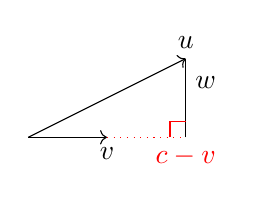
\begin{tikzpicture}
		\draw[->] (0, 0) -- (2, 1) node[anchor=south] {$u$};
		\draw[->] (0, 0) -- (1, 0) node[anchor=north] {$v$};
		\draw (2, 0) -- (2, 1) node[midway, anchor=south west] {$w$};
		\draw[dotted, red] (1, 0) -- (2, 0) node[anchor=north] {$c - v$};
		\draw[red] (1.8, 0) -- (1.8, 0.2) -- (2, 0.2);
	\end{tikzpicture}

	Want:

	\begin{align*}
		\left<w, v \right> & \iff \left<u - c \cdot v, v \right> = 0                                 \\
		                   & \iff \left<u, v \right> - c \cdot \left<v, v \right> = 0                \\
		                   & \iff \left< u, v \right> - c \cdot \left\lVert v \right\rVert^{2} = 0   \\
		                   & \implies c = \frac{\left< u, v \right>}{\left\lVert v \right\rVert^{2}} \\
	\end{align*}

	\nt{

		\[
			w = u - cv = u - \frac{\left< u, v \right>}{\left\lVert v \right\rVert^{2}} \cdot v
		\]

		Where \(v\) and \(w\) are orthogonal.
	}
}

\thm{Cauchy-Schwarz inequality}{
	Suppose that \(V\) is an inner product space and \(u, v \in V\). Then:

	\[
		\left\lvert \left< u, v \right> \right\rvert \le \left\lVert u \right\rVert \cdot \left\lVert v \right\rVert
	\]

	With equality if and only if \(u\) and \(v\) are linearly dependent.

	\pf{Proof}{
		If \(v = \vec{0_{v}} \), then both sides are \(0_{\FF}\).

		\nt{
			In this case equality holds and \(u, v\) are linearly dependent.
		}

		If \(v \neq \vec{0_{v}} \), then \(v\) and \(w \coloneq u - \frac{\left< u, v \right>}{\left\lVert v \right\rVert^{2}} \cdot v\) are orthogonal.

		Which means so are \(\alpha \cdot v\) and \(w\) for any \(\alpha \in \FF\).

		Recall that Pythagoras:

		\[
			\left\lVert w + \alpha \cdot v \right\rVert^{2} = \left\lVert w \right\rVert^{2} + \left\lVert \alpha v \right\rVert^{2} = \left\lVert w \right\rVert^{2} + \left\lvert \alpha \right\rvert^{2} \cdot \left\lVert v \right\rVert^{2}
		\]



		Pick \(\alpha = \frac{\left< u, v \right>}{\left\lVert v \right\rVert^{2}}\), so that \(w + \alpha v = u\)


		This implies that:

		\[
			\left\lVert u \right\rVert^{2} = \left\lVert w \right\rVert^{2} + \left\lvert \frac{\left< u, v \right>}{\left\lVert v \right\rVert^{2}} \right\rvert^{2} \cdot \left\lVert v \right\rVert^{2}
		\]

		Where the right term of the sum is:

		\[
			\frac{\left\lvert \left<u, v \right> \right\rvert^{2}}{\left\lVert v \right\rVert^{4}} \cdot \left\lVert v \right\rVert^{2}
		\]

		Which is:

		\[
			\left\lVert v \right\rVert^{2} = \left\lVert w \right\rVert^{2} + \frac{\left\lvert \left<u, v \right> \right\rvert^{2}}{\left\lVert v \right\rVert^{2}} \geq \frac{\left\lvert \left<u, v \right> \right\rvert^{2}}{\left\lVert v \right\rVert^{2}}
		\]

		So we get:

		\[
			\left\lVert v \right\rVert^{2} \geq \frac{\left\lvert \left<u, v \right> \right\rvert^{2}}{\left\lVert v \right\rVert^{2}} \implies \left\lVert u \right\rVert \cdot \left\lVert v \right\rVert \geq \left\lvert \left<u, v \right> \right\rvert
		\]

		Notice that equality holds if and only if:

		\begin{align*}
			\left\lVert w \right\rVert = 0 & \iff w = \vec{0_{v}}                                                                                                 \\
			                               & \iff u = \frac{\left< u, v \right>}{\left\lVert v \right\rVert^{2}} \cdot v = 0                                      \\
			                               & \iff u = \frac{\left< u, v \right>}{\left\lVert v \right\rVert^{2}} \cdot v \iff u, v \text{ are linearly dependent}
		\end{align*}



	}
}

\ex{}{
	\begin{enumerate}[wide]
		\item Let \(V = \RR^{n}, \FF = \RR, \left<\,,\, \right> = \) dot product.

		      \begin{align*}
			      \vec{x}  = (x_1, \ldots, x_{n}) \\
			      \vec{y}  = (y_1, \ldots, y_{n}) \\
		      \end{align*}

		      C.S. tell us:

		      \begin{align*}
			      \left\lvert \left< \vec{x}, \vec{y} \right> \right\rvert^{2} & \leq \left\lVert \vec{x} \right\rVert^{2} \cdot \left\lVert \vec{y} \right\rVert^{2} \\
			      (x_1y_1 + \ldots + x_{n}y_{n})^{2}                           & \leq (x_{1}^{2} + \ldots + x_{n}^{2}) \cdot (y_{1}^{2} + \ldots + y_{n}^{2})         \\
		      \end{align*}
		\item Let \(V = \left\{ f : [-1, 1] \to \RR \mid f \text{ is continuous} \right\}, \FF = \RR, \left< f, g \right> = \int_{-1}^{1} f(x)g(x) dx\).

		      By C.S., we know that:

		      \[
			      \left\lvert \left< f, g \right> \right\rvert^{2} \leq \left\lVert f \right\rVert^{2} \cdot \left\lVert g \right\rVert^{2}
		      \]

		      Thus:

		      \begin{align*}
			      \left(\int_{-1}^{1} f(x)g(x) dx\right)^{2} & \leq \left(\int_{-1}^{1} f(x)^{2} dx\right) \cdot \left(\int_{-1}^{1} g(x)^{2} dx\right) \\
		      \end{align*}
	\end{enumerate}
}

\thm{Triangle Inequality}{

	Given \(u, v\) in an inner product space \(V\), we have:

	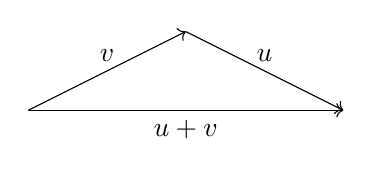
\begin{tikzpicture}
		\draw[->] (0, 0) -- (2, 1) node[midway, above] {$v$};
		\draw[->] (2, 1) -- (4, 0) node[midway, above] {$u$};
		\draw[->] (0, 0) -- (4, 0) node[midway, below] {$u + v$};
	\end{tikzpicture}

	The triangle inequality states that:

	\[
		\left\lVert u + v \right\rVert \leq \left\lVert u \right\rVert + \left\lVert v \right\rVert
	\]

	\pf{Proof}{

		\begin{align*}
			\left\lVert u + v \right\rVert^{2} & = \left< u + v, u + v \right>                                                                                                                         \\
			                                   & = \left< u, u\right> + \left< u, v \right> + \left< v, u \right> + \left< v, v \right>                                                                \\
			                                   & = \left\lVert u \right\rVert^{2} + \left<u, v \right>+ \overline{\left<u, v \right>} + \left\lVert v \right\rVert^{2}                                 \\
			                                   & = \left\lVert u \right\rVert^{2} + 2 \cdot \operatorname{Re}\left<u, v \right> + \left\lVert v \right\rVert^{2} \text{ as } (a + bi) + (a - bi) = 2a  \\
			&\le \left\lVert u \right\rVert^{2} + 2 \cdot \left\lvert \left< u, v \right> \right\rvert + \left\lVert v \right\rVert^{2}\text{ by } \star               \\
			&\le \left\lVert u \right\rVert^{2} + 2 \cdot \left\lVert u \right\rVert \cdot \left\lVert v \right\rVert + \left\lVert v \right\rVert^{2} \text{ by C.S.} \\
			&= \left(\left\lVert u \right\rVert + \left\lVert v \right\rVert\right)^{2}
		\end{align*}

		Thus, we get:

		\begin{align*}
			\left\lVert u + v \right\rVert^{2} & \leq \left(\left\lVert u \right\rVert + \left\lVert v \right\rVert\right)^{2} \\
			\left\lVert u + v \right\rVert     & \leq \left\lVert u \right\rVert + \left\lVert v \right\rVert
		\end{align*}

		So why is \(\star\) true?

		\begin{align*}
			\left< u, v \right> = a + bi &\implies \left\lvert \left< u, v \right> \right\rvert = \sqrt{a^{2} + b^{2}} \\
			\operatorname{Re}\left<u, v \right> &= a
		\end{align*}

		But why is \(a \leq \sqrt{a^{2} + b^{2}}\)?

		True since:

		\begin{align*}
			a &\le \left\lvert a \right\rvert \\
			  &= \sqrt{a^{2}} \\
			  &\le \sqrt{a^{2} + b^{2}}
		\end{align*}

		Which means the triangle inequality holds.
	}
}

\ex{}{
	Let \(V = \RR^{n}, \vec{x} = (x_1, \ldots, x_{n}), \vec{y} = (y_1, \ldots, y_{n})\).

	We have:

	\[
		\left\lVert \vec{x} + \vec{y} \right\rVert^{2} = \left\lVert \vec{x} \right\rVert^{2} + 2 \cdot \left< \vec{x}, \vec{y} \right> + \left\lVert \vec{y} \right\rVert^{2}
	\] 

	Thus:

	\begin{align*}
		\sum_{i=1}^{n} (x_{i} + y_{i})^{2} &\leq \left(\sqrt{\sum_{i=1}^{n} x_{i}^{2}} + \sqrt{\sum_{i=1}^{n} y_{i}^{2}}\right)^{2} \\
		&= \sum_{i=1}^{n} x_{i}^{2} + 2 \cdot \sqrt{\sum_{i=1}^{n} x_{i}^{2}} \cdot \sqrt{\sum_{i=1}^{n} y_{i}^{2}} + \sum_{i=1}^{n} y_{i}^{2} \\
	\end{align*}
}


\section{Orthonormal bases}

\dfn{}{
	Let \(V\) be an inner product space over \(\FF\).

	Let \(e_1, \ldots, e_{n} \) be a list of vectors in \(V\).

	Then we say \(\left\{ e_1, \ldots, e_{n} \right\}\) is an orthogonal list if:

	\[
		\left< e_i, e_j \right> = \delta_{ij} \coloneq \begin{cases}
			1_{\FF} & i = j    \\
			0_{\FF} & i \neq j
		\end{cases}
	\] 

	E.g.

	\begin{align*}
		\left( \frac{1}{\sqrt{3} }, \frac{1}{\sqrt{3} }, \frac{1}{\sqrt{3} } \right), \left( -\frac{1}{\sqrt{2} }, \frac{1}{\sqrt{2} }, 0 \right) \in \RR^{3} \\
	\end{align*}

	We normalize the vectors to get a length of \(1\).

	If an orthogonal list is also a basis, then the following holds:

	\begin{align*}
		\left\lVert a_1 e_1 + \ldots + a_{n} e_{n} \right\rVert^{2} &= \left< a_1 e_1 + \ldots + a_{n} e_{n}, a_1 e_1 + \ldots + a_{n} e_{n} \right> \\
		&= \left<a_1 e_1, a_1 e_1\right> + \ldots + \left<a_{n} e_{n}, a_{n} e_{n}\right> \\
		&= a_1 \cdot \overline{a_1} \left<e_1, e_1 \right> + \ldots + a_{n} \cdot \overline{a_{n}} \left<e_{n}, e_{n}\right> \\
		&= \left\lvert a_1 \right\rvert^{2} + \ldots + \left\lvert a_{n} \right\rvert^{2} \\
	\end{align*}

	A list of orgthogonal vectors is linearly independent, but might not span.
}




\dfn{}{

	\(V\) is an inner product space over \(\RR\) or \(\CC\).

	Then we say \(\left\{ V_1, \ldots, V_{n} \right\}\) is an orthonormal if :

	\[
		\left< V_{i}, V_{j} \right> = \begin{cases}
			1_{\FF} & i = j    \\
			0_{\FF} & i \neq j
		\end{cases}
	\]

}

\clm{}{}{
Suppose \(\left\{ V_{1}, \ldots, V_{n} \right\}\) is orthonormal, then \(\left\{ V_{1}, \ldots, V_{n} \right\}\) is linearly independent.

\pf{Proof}{
	Suppose there are some scalars \(c_1, \ldots, c_{n} \in \FF\) such that:

	\[
		c_1 v_1 + \ldots c_{n} v_{n} = 0
	\]
	Then it follows:

	\[
		\left< c_1 v_1 + \ldots c_{n} v_{n}, c_1 v_1 + \ldots c_{n} v_{n} \right>       = \left\lVert c_1 v_1 + \ldots c_{n} v_{n} \right\rVert^{2}                                  = 0
	\]

	Which means:

	\[
		\left\lvert c_1 \right\rvert^{2} + \ldots + \left\lvert c_{n} \right\rvert^{2} = 0 \implies \left\lvert c_1 \right\rvert^{2} = \ldots = \left\lvert c_{n} \right\rvert^{2}  = 0
	\]

	Thus,

	\[
	c_1 = \ldots = c_{n} = 0_{\FF}
			\]
		}
}

\mclm{}{
	Suppose \(\left\{ e_1, \ldots, e_{n} \right\}\) is an orthonormal basis for \(V\). and let \(v \in V\). Then:
}



\begin{algorithm}[H]
	\KwIn{\(\vec{v_1}, \ldots, \vec{v_n}  \in V\). Linearly independent set. }
	\KwOut{\(e_1, \ldots, e_{n} \in V\) orthonormal basis and \(\operatorname{span}\left( e_1, \ldots, e_{n} \right) = \operatorname{span}\left( v_1, \ldots, v_{n} \right)\)}
	\vspace{5mm}
	\SetAlgoLined{}
	\tcc{We want \(\left< e_1, e_2 \right> = 0_{\FF}\)}
	\(\vec{e_1} = \frac{\vec{v_1}}{\left\lVert \vec{v_1} \right\rVert}\)\;
	\(\vec{e_2} = \frac{\vec{v_2} - \left< \vec{v_2}, \vec{e_1} \right> \cdot \vec{e_1}}{\left\lVert \vec{v_2} - \left< \vec{v_2}, \vec{e_1} \right> \cdot \vec{e_1} \right\rVert}\)\;
	\(\vec{e_j} = \frac{\vec{v_j} - \left< \vec{v_j}, \vec{e_1} \right> \cdot \vec{e_1} - \ldots - \left< \vec{v_j}, \vec{e_{j-1}} \right> \cdot \vec{e_{j-1}}}{\left\lVert \vec{v_j} - \left< \vec{v_j}, \vec{e_1} \right> \cdot \vec{e_1} - \ldots - \left< \vec{v_j}, \vec{e_{j-1}} \right> \cdot \vec{e_{j-1}} \right\rVert}\)\;
	\caption{Gram-Schmidt Process}
\end{algorithm}

\ex{}{
	Let \(V = \mcP_{2}(\RR), \left< p, q \right> = \int_{-1}^{1} p(x)q(x) dx\).

	Start with \(\vec{v_1} = 1, \vec{v_2} = x, \vec{v_3} = x^{2}\).

	\begin{enumerate}[wide]
		\item

		      \begin{align*}
			      \vec{e_1} & = \frac{\vec{v_1}}{\left\lVert \vec{v_1} \right\rVert} = \int_{-1}^{1} 1^{2} dx = \sqrt{2} \\
			                & = \frac{1}{\sqrt{2}}
		      \end{align*}
		\item

		      \begin{align*}
			      v_2 - \left< v_2, e_1 \right> \cdot e_1 & = x - \int_{-1}^{1} x \cdot \frac{1}{\sqrt{2}} dx \cdot \frac{1}{\sqrt{2}} \\
			                                              & \text{notice that the integral is 0 as \(x\) is odd}                       \\
			                                              & = x
		      \end{align*}

		      Remember that:

		      \[
			      \vec{e_2} = \frac{\vec{v_2} - \left< \vec{v_2}, \vec{e_1} \right> \cdot \vec{e_1}}{\left\lVert \vec{v_2} - \left< \vec{v_2}, \vec{e_1} \right> \cdot \vec{e_1} \right\rVert} = \frac{x}{\left\lVert x \right\rVert}
		      \]

		      \begin{align*}
			      \left\lVert x \right\rVert^{2} = \left< x, x\right>      & = \int_{-1}^{1} x^{2} dx = \frac{2}{3}            \\
			      \implies \left\lVert x \right\rVert = \sqrt{\frac{2}{3}} & \implies \vec{e_2} = \frac{x}{\sqrt{\frac{2}{3}}}
		      \end{align*}

		\item

		      \begin{align*}
			      v_3 - \left< v_3, e_1 \right> \cdot e_1 - \left< v_3, e_2 \right> \cdot e_2 & = x^{2} - \int_{-1}^{1} x^{2} \cdot \frac{1}{\sqrt{2}} dx \cdot \frac{1}{\sqrt{2}} - \int_{-1}^{1} x^{2} \cdot \frac{x}{\sqrt{\frac{2}{3}}} dx \cdot \frac{x}{\sqrt{\frac{2}{3}}} \\
			                                                                                  & \text{notice that the integral is 0 as the right side is odd}                                                                                                                     \\
			                                                                                  & = x_2 - \frac{1}{3}
		      \end{align*}

		      Hence,

		      \[
			      \left\lVert x^{2} - \frac{1}{3} \right\rVert = \sqrt{\int_{-1}^{1} (x^{2} - \frac{1}{3})^{2} dx} = \sqrt{\frac{8}{45}} \implies \vec{e_3} = \frac{x^{2} - \frac{1}{3}}{\sqrt{\frac{8}{45}}}
		      \]
	\end{enumerate}
}

\mclm{This week}{
	\begin{enumerate}[label=(\roman*)]
		\item Inner product spaces
		\item Some properties:

		      \[
			      u = 0 \iff \left< v, u \right> = 0 \text{ for all } v \in V
		      \]

		      In particular:

		      \begin{align*}
			      u                                              & = u' \\
			      \iff u - u'                                    & = 0  \\
			      \iff \forall v \in V, \left< v, u - u' \right> & = 0  \\
		      \end{align*}
	\end{enumerate}
}

\mclm{Goal}{
	Study linear operators between inner product spaces
}

\dfn{}{
	A linear functional on \(V\) is a linear map \(V \xrightarrow{\phi} \FF\).

	i.e., \(\phi \in \sL(V, \FF)\)
}

% \ex{}{
% 	Let \(\phi: \FF^{3}\) 
% }

\thm{Riesz Representation Theorem (RRT)}{
	Let \(V\) be a finite-dimensional vector space over \(\FF\) and \(\phi \in \sL(V, \FF)\).

	Then there exists a unique \(u \in V\) such that:

	\[
		\phi(v) = \left< v, u \right> \text{ for all } v \in V
	\]

	\pf{Proof of part \(1\)}{
		Find \(u\).

		\[
			\phi(v) = \phi(\left< v, e_1 \right> e_1 + \ldots + \left< v, e_{n} \right> e_{n})
		\]

		For some orthonormal basis \(\left\{ e_1, \ldots, e_{n} \right\}\) of \(V\).

		This means we get:

		\begin{align*}
			 & = \left< v, e_1 \right> \phi(e_1) + \ldots + \left< v, e_{n} \right> \phi(e_{n})                       \\
			 & = \left< v, \overline{\phi(e_1)} e_1 \right> + \ldots + \left< v, \overline{\phi(e_{n})} e_{n} \right> \\
			 & = \left<v, \overline{\phi(e_1)} e_1 + \ldots + \overline{\phi(e_{n})} e_{n} \right>                    \\
		\end{align*}

		Which is \(u\)!

		Thus,

		\[
			\phi(v) = \left< v, u \right> \text{ for all } v \in V
		\]

	}

	\pf{Uniqueness}{

		\[
			\phi(v) = \left< v, u \right> = \left< v, u' \right> \text{ for all } v \in V
		\]

		Show \(u = u' \iff\) show \(\left< v, u - u' \right> = 0\) for all \(v \in V\).

		\begin{align*}
			\left< v, u - u' \right> & = \left< v, u \right> - \left< v, u' \right> \\
			                         & = \phi(v) - \phi(v)                          \\
			                         & = 0
		\end{align*}

		Thus, \(u = u'\).
	}

	\nt{
		Because of uniqueness the \(u\) in the proof cannot / doesn't depend on the choice of basis.
	}
}

\ex{}{
	Let \(\mcP_{2}(\RR)\) with \(\left< p, q \right> = \int_{-1}^{1} p(x)q(x) dx\).

	This has an orthonormal basis:

	\[
		e_1 = \sqrt{\frac{1}{2}} , e_2 = \sqrt{\frac{3}{2}} x, e_3 = \sqrt{\frac{45}{8}} (x^{2} - \frac{1}{3})
	\]

	Let \(\phi \in \sL(\mcP_{2}(\RR), \RR)\) be defined by:

	\[
		\phi(p) = \int_{-1}^{1} p(x)\cos(\pi x) dx \in \sL(\mcP_{2}(\RR), \RR)
	\]

	\nt{

		We have:

		\[
			\left< p, \cos(\pi x) \right> = \phi(p)
		\]

		but \(\cos(\pi x) \notin \mcP_{2}(\RR)\).
	}

	Thus, by using RRT,

	\[
		\phi(p) = \left< p, u \right>
	\]

	Where \(u = \overline{\phi(e_1)} e_1 + \overline{\phi(e_2)} e_2 + \overline{\phi(e_3)} e_3\).

	Notice that the second term is

	\[
		\overline{\phi(e_2)} e_2 = \overline{\int_{-1}^{1} x \cos(\pi x) dx} \cdot \sqrt{\frac{3}{2}} x
	\]

	Computing gives us:

	\[
		u = -\frac{45}{2\pi^{2}} (x^{2} - \frac{1}{3})
	\]
}

Now, let \((V, \left<\,,\, \right>_{V}), (W, \left<\,,\, \right>_{W})\) be inner product spaces over \(\FF\).

Let \(T \in \sL(V, W)\).

For each \(w \in W\), create: \(\phi_{w} \in \sL(V, \FF)\) by:

\[
	\phi_{w}(v) = \left< T(v), w \right>_{W}
\]

By RRT, for all \(w \in W\), there exists a unique \(u_{w} \in V\) such that:


\[
	\phi_{w}(v) = \left< v, u_{w} \right>_{V}
\]

Now, notice:

\[
	\left< v, u_{w} \right>_{V} = \left< T(v), w \right>_{W}
\]

By uniqueness of \(u_{w}\), we can define:


\[
	T^{*}: W \to V, w \mapsto u_{w} \coloneq T^{*}(w)
\]

\dfn{}{
	The adjoint of a linear map \(T: V \to W\) between inner product spaces is the linear map \(T^{*}: W \to V\) characterized by:

	\[
		\left< T(v), w \right>_{W} = \left< v, T^{*}(w) \right>_{V}
	\]
}

\ex{}{
	Let \(\RR^{3}, \RR^{2}\) with the standard inner product i.e., dot product.

	\[
		T: \RR^{3} \to \RR^{2},\quad T(x_1, x_2, x_3) = (x_1 + x_2, 2x_2 + x_3)
	\]

	What is \(T^{*}: \RR^{2} \to \RR^{3}\)?


	\begin{align*}
		\left< T(x_1, x_2, x_3), (y_1, y_2) \right>_{\RR^{2}} & = \left< (x_1 + x_2, 2x_2 + x_3), (y_1, y_2) \right>_{\RR^{2}}     \\
		                                                      & = \left< (x_1, x_2, x_3), T^{*}(y_1, y_2) \right>_{\RR^{3}}        \\
		                                                      & = (x_1 + x_2)y_1 + (2x_2 + x_3)y_2                                 \\
		                                                      & = x_1y_1 + x_2y_1 + 2x_2y_2 + x_3y_2
		                                                      & = \left< (x_1, x_2, x_3), (y_1, y_1 + 2y_2, y_2) \right>_{\RR^{3}}
	\end{align*}

	Thus, \(T^{*}(y_1, y_2) = (y_1, y_1 + 2y_2, y_2)\).
}

\nt{
	Is \(T^{*}\) is linear?

	Adjoins are linear:

	If \(T: V \to W\) is linear, then \(T^{*}: W \to V\) is linear.
}


% chapter 7
\chapter{Operators on Inner Product Spaces}


% chapter 8
\chapter{Operators on Complex Vector Spaces}


% chapter 9
\chapter{Operators on Real Vector Spaces}


% chapter 10
\chapter{Determinants and Traces}

\section{Determinants and Permutations}
\label{sec:det}

\dfn{Determinants}{

	\(\det : \FF^{n, n} \implies \FF\)

	\begin{enumerate}[label=(\alph*)]
		\item If \(n = 1\), then \(\det (a) = a\).
		\item If \(n = 2\), then \(\det \begin{pmatrix} a & b \\ c & d \end{pmatrix} = ad - bc\).
		\item If \(n \ge 3\), then we need a recursive definition.

		      If \(A \in \FF^{n, n}\), then the \(ij\)-th minor of \(A\) is \(A_{i,j}\).

		      Where \(A_{i,j}\) means you take \(A\) and delete the \(i\)th row and \(j\)th column.

		      \ex{}{

			      Let \[A = \begin{pmatrix} 1 & 2 & 3 \\ 4 & 5 & 6 \\ 7 & 8 & 9 \end{pmatrix}\].

			      Then:

			      \[
				      A_{2,1} = \begin{pmatrix} 2 & 3 \\ 8 & 9 \end{pmatrix}
			      \]

		      }

		      Thus, given \(A \in \FF^{n, n}\), define its determinant as:

		      \[
			      \det A = \sum_{i = 1}^{n} (-1)^{i + 1} a_{i,1} \cdot \det A_{i,1}
		      \]
	\end{enumerate}
}

\newpage
\ex{}{
	Let:

	\[
		A = \begin{pmatrix} 1 & 0 & 3 \\ 2 & 1 & 2 \\ 0 & 5 & 1 \end{pmatrix} = \begin{pmatrix} a_{11} & a_{12} & a_{13} \\ a_{21} & a_{22} & a_{23} \\ a_{31} & a_{32} & a_{33} \end{pmatrix}
	\]

	Thus,

	\begin{align*}
		\det A & = a_{1,1} \cdot \det A_{1,1} - a_{2, 1} \cdot \det A_{2,1} + a_{3,1} \cdot \det A_{3,1}                                                                                             \\
		       & = 1 \cdot \det \begin{pmatrix} 1 & 2 \\ 5 & 1 \end{pmatrix} - 2 \cdot \det \begin{pmatrix} 0 & 3 \\ 5 & 1 \end{pmatrix} + 0 \cdot \det \begin{pmatrix} 0 & 3 \\ 1 & 2 \end{pmatrix} \\
		       & = 1 \cdot (-9) - 2 \cdot (-15) + 0 \cdot (-3)                                                                                                                                       \\
		       & = 21
	\end{align*}
}

\thm{Det 1}{
	There exists a unique function \(\delta : \FF^{n, n} \to \FF\) with the following properties:

	\begin{enumerate}
		\item \(\delta(I_{n}) = 1\)
		\item \(\delta\) is row-linear.
		\item If \(A\) has two identical rows, then \(\delta(A) = 0\).
	\end{enumerate}

	Point: we will show that \(\det = \delta\).

	\mclm{Row-linear}{
		This means that:

		\[
			\delta \left( \begin{pmatrix}  1 & 2 & 3\\ 4\lambda + 2\mu & 5\lambda + 5\mu & 6\lambda + 8\mu \\ 7 & 8 & 9 \end{pmatrix} \right) = \lambda \cdot \delta \begin{pmatrix} 1 & 2 & 3 \\ 4 & 5 & 6 \\ 7 & 8 & 9 \end{pmatrix}  + \mu \cdot \delta  \begin{pmatrix} 1 & 2 & 3 \\ 2 & 5 & 8 \\ 7 & 8 & 9 \end{pmatrix}
		\]

		Assume the previous theorem is true for now.

		What is the value of \(\delta\) on elementary matrices?
	}
}

\thm{Det 2}{

	\(E\) elementary matrix. Then:

	\[
		\delta(E \cdot A) = \begin{cases}
			\delta(A)         & \text{ if } E \text{ is type (i)}   \\
			-\delta(A)        & \text{ if } E \text{ is type (ii)}  \\
			c \cdot \delta(A) & \text{ if } E \text{ is type (iii)}
		\end{cases}
	\]

	\(S\) is determined on elementary matrices.
}

\cor{Related to thm 2}{

	\[
		\delta(E) = \begin{cases}
			+1 & \text{ if } E \text{ is type (i)}   \\
			-1 & \text{ if } E \text{ is type (ii)}  \\
			c  & \text{ if } E \text{ is type (iii)}
		\end{cases}
	\]

	\pf{Proof}{
		Take \(A = I_{n}\) in theorem 2.
	}

}

\newpage

\pf{Proof to det 2}{

	For \(E\) of type \((iii)\) this is jut row-linearity of \(\delta\).

	Let \(A_{i}\) be the \(i\)th row of \(A\).

	\[
		\delta \left( \begin{pmatrix} 1 & & & & \\ & \ddots & & & \\ & & c & & \\ & & & \ddots & \\ & & & & 1 \end{pmatrix} \cdot \begin{pmatrix} -- & A_1 & -- \\ -- & A_2 & -- \\  & \vdots &  \\ -- & A_n & -- \end{pmatrix} \right) = \delta \begin{pmatrix} -- & A_1 & -- \\  & \vdots &  \\ -- & cA_i & -- \\  & \vdots &  \\ -- & A_n & -- \end{pmatrix} = c \cdot \delta \begin{pmatrix} -- & A_1 & -- \\  & \vdots &  \\ -- & A_i & -- \\  & \vdots &  \\ -- & A_n & -- \end{pmatrix} = c \cdot \delta(A) \begin{pmatrix} 1 & & & & \\ & \ddots & & & \\ & & c & & \\ & & & \ddots & \\ & & & & 1 \end{pmatrix}
	\]

	Since we did not require \(c \neq 0\), then this is true for all \(c \in \FF\).

	Thus, \(\delta(E \cdot A) = c \cdot \delta(A)\) for all \(c \in \FF\).

	If a row contains only zeros, then \(\delta(A) = 0\).

	For types \((i)\) and \((ii)\), we do the special case when \(E\) acts on consecutive rows.

	\begin{enumerate}[label=(Type: \roman*):, wide]
		\item

		      \[
			      E \cdot A = \begin{pmatrix} 1 & & & & \\ & \ddots & & a_{i,j} & \\ & & \ddots & & \\ & & & \ddots & \\ & & & & 1\end{pmatrix} \cdot \begin{pmatrix} -- & A_1 & -- \\ -- & A_2 & -- \\  & \vdots &  \\ -- & A_i & -- \\ -- & A_{i+1} & -- \\  & \vdots &  \\ -- & A_n & -- \end{pmatrix} = \begin{pmatrix} -- & A_1 & -- \\ -- & A_2 & -- \\  & \vdots &  \\ -- & a_{i,j} A_i + A_{j} & -- \\ -- & A_{i+1} & -- \\  & \vdots &  \\ -- & A_n & -- \end{pmatrix}
		      \]

		      Special case, \(j = i + 1\)

		      \[
			      \delta(E \cdot A) = \delta\begin{pmatrix} -- & A_1 & -- \\ -- & A_2 & -- \\  & \vdots &  \\ -- & A_{i+1} & -- \\ -- & aA_i + A_{i+1} & -- \\   & \vdots &  \\ -- & A_n & -- \end{pmatrix} = a \cdot \delta \begin{pmatrix} -- & A_1 & -- \\ -- & A_2 & -- \\  & \vdots &  \\ -- & A_i & -- \\ -- & A_i & -- \\  & \vdots &  \\ -- & A_n & -- \end{pmatrix} + \delta \begin{pmatrix} -- & A_1 & -- \\ -- & A_2 & -- \\  & \vdots &  \\ -- & A_i & -- \\ -- & A_{i+1} & -- \\  & \vdots &  \\ -- & A_n & -- \end{pmatrix}
		      \]

		      But, the first matrix's determinant is \(0\) since it has two identical rows.

		      Thus, \(\delta(E \cdot A) = a \cdot 0 + \delta(A) = \delta(A)\).
		\item Swap rows.

		      Again, this assumes theorem \(1\).

		      Let's assume that we swap row \(i\) with row \(i + 1\)

		      {\allowdisplaybreaks
				      \begin{align*}
					      \delta(A) & = \delta \begin{pmatrix} -- & A_1 & -- \\ & \vdots &  \\ -- & A_i & -- \\ -- & A_{i+1} & -- \\  & \vdots &  \\ -- & A_n & -- \end{pmatrix}                                                                                                                                              \\
					                & \text{ by part one:}                                                                                                                                                                                                                                                                    \\
					                & = \delta \begin{pmatrix} -- & A_1 & -- \\ & \vdots &  \\ -- & A_{i} - A_{i+1} & -- \\ -- & A_{i+1} & -- \\  & \vdots &  \\ -- & A_n & -- \end{pmatrix}                                                                                                                                  \\
					                & \text{ by part one again:}                                                                                                                                                                                                                                                              \\
					                & = \delta \begin{pmatrix} -- & A_1 & -- \\ & \vdots &  \\ -- & A_{i} - A_{i+1} & -- \\ -- & A_{i + 1} + \left(A_{i} - A_{i+1}\right) & -- \\  & \vdots &  \\ -- & A_n & -- \end{pmatrix}                                                                                                 \\
					                & = \delta \begin{pmatrix} -- & A_1 & -- \\ & \vdots &  \\ -- & A_{i} - A_{i+1} & -- \\ -- & A_{i} & -- \\  & \vdots &  \\ -- & A_n & -- \end{pmatrix}                                                                                                                                    \\
					                & \text{ by row linearity:}                                                                                                                                                                                                                                                               \\
					                & = \delta \begin{pmatrix} -- & A_1 & -- \\ & \vdots &  \\ -- & A_{i} & -- \\ -- & A_{i} & -- \\  & \vdots &  \\ -- & A_n & -- \end{pmatrix} - \delta \begin{pmatrix} -- & A_1 & -- \\ & \vdots &  \\ -- & A_{i+1} & -- \\ -- & A_{i} & -- \\  & \vdots &  \\ -- & A_n & -- \end{pmatrix} \\
					                & \text{but for the first matrix is zero since it has two identical rows:}                                                                                                                                                                                                                \\
					                & = -\delta \begin{pmatrix} -- & A_1 & -- \\ & \vdots &  \\ -- & A_{i+1} & -- \\ -- & A_{i} & -- \\  & \vdots &  \\ -- & A_n & -- \end{pmatrix}                                                                                                                                           \\
					                & = - \delta(E \cdot A)
				      \end{align*}

				      Thus, \(\delta(A) = - \delta(E \cdot A)\), which implies

				      \[
					      \delta(E \cdot A) = - \delta(A)
				      \]
			      }
	\end{enumerate}

	In general, for part \(2\), we want to swap \(i\) with row \(j\).

	Assume \(i < j\).

	\begin{enumerate}[label=(\roman*), wide]
		\item We bubble down row \(i\) to row \(j\) indices \(j-1\) exchanges.

		      Thus, row \(i\) is in the right place.

		      But Row \(j\) is row in Row \(j - 1\).
		\item Bubble up row \(j\) (in position \(j -1\)  right now) to row \(i\).

		      This involves \((j - 1) - i\) exchanges.

		      Which means that the total number of exchanges is:

		      \[
			      j - 1 + (j - 1) - i = 2(j - i) - 1
		      \]

		      Which is odd!

		      This means that \(\delta(E \cdot A) = (-1)^{2(j - i) - 1} \cdot \delta(A) = - \delta(A)\).
	\end{enumerate}

	\nt{
		We can also do this for part \(1\).

		Do this an exercise.
	}

	As such, we have proven theorem \(2\).
}

\cor{}{
	\(\delta(S \cdot B) = \delta(A) \cdot \delta(B)\) for any \(A, B \in \FF^{n, n}\).

	We know that \(\delta(E) \cdot \delta(A) = \delta(E \cdot A)\) if \(E\) is an elementary matrix.

	Let \(A^{\prime} = E_{k} \cdots E_{1} \cdot A\)  be a reduced row echelon form of \(A\).

	Then either:

	\begin{enumerate}[label=(\roman*), wide]
		\item \(A^{\prime} = I_{n}\) or
		\item the last row of \(A^{\prime}\) is all zeros. (could be more than the last row)
	\end{enumerate}

	Then:

	\begin{enumerate}[label=(\roman*)]
		\item If \(A^{\prime} = I_{n}\),

		      \begin{align*}
			      A^{\prime} = I_{n} & \implies A = E_{1}^{-1} \cdots E_{k}^{-1} \cdot I_{n}             \\
			                         & \implies \delta(A) = \delta(E_{1}^{-1}) \cdots \delta(E_{k}^{-1})
		      \end{align*}

		      On the other hand:

		      \begin{align*}
			      \delta(A \cdot B) & = \delta(E^{-1}_{1}) \cdots \lambda(E^{-1}_{k}) \cdot \delta(B) \\
			                        & = \delta(A) \cdot \delta(B)
		      \end{align*}
		\item If \(A^{\prime}\) has a row of zeros, then:

		      \(\delta(A^{\prime}) = 0\), which implies that \(\delta(A) = 0\).

		      Since \(\delta(A^{\prime}) = \delta(E_{k}) \cdots \delta(E_{1}) \cdot \delta(A)\).

		      Where \(\delta(E_{i}) \neq 0\) for all \(i\).

		      This implies that \(\delta(A) = 0\).

		      And exercise: \(\delta(A \cdot B) = 0\) as well.
	\end{enumerate}

}

\pf{Proof of det 1}{

	\pf{Proof of uniqueness}{
		Suppose there are functions \(\delta: \FF^{n, n} \to \FF\) and \(\delta^{\prime} : \FF^{n, n} \to \FF\).

		Each satisfying the three desired properties.

		Let \(A \in \FF^{n, n}\) such that \(A^{\prime} = E_{k} \cdots E_{1} \cdot A\) is a reduced row echelon form of \(A\).

		Either we get \(A^{\prime} = I_{n}\) or its last row is all zeros.

		In either case, \(\delta(A^{\prime}) = \delta^{\prime}(A^{\prime}) = 1\).

		Or \(\delta(A^{\prime}) = \delta^{\prime}(A^{\prime}) = 0\).

		That means that \(\delta(E_{k} \cdots E_{1} \cdot A)  = \delta^{\prime}(E_{k} \cdots E_{1} \cdot A)\) in either case.

		Thus,
		\[
			\delta(E_{k}) \cdots \delta(E_{1}) \cdot \delta(A) = \delta^{\prime}(E_{k}) \cdots \delta^{\prime}(E_{1}) \cdot \delta^{\prime}(A)
		\]

		But by theorem \(2\), we get \(\delta(E_{i}) = \delta^{\prime}(E_{i})\).

		Which means that \(\delta(A) = \delta^{\prime}(A)\) for all \(A \in \FF^{n, n}\).
	}

	\pf{Proof of existence}{
		We'll show \(\det : \FF^{n,n} \to \FF\) satisfies the three properties to be \(\delta\).

		Let's proceed by induction on \(n \in \NN\)

		\mclm{Base Case}{
			Let \(n\) be \(1\).

			Then \(\det : \FF^{1,1} \to \FF\) is defined by \(\det(a) = a\).

			Thus, \(\det(I_{1}) = 1\).

			Now, for row linear:

			\[
				\det(\lambda a + \mu b) = \lambda \cdot \det(a) + \mu \cdot \det(b)
			\]

			Part \(3\) is trivial since there is only one row.
		}

		\mclm{Inductive Step}{
			Assume that \(\det : \FF^{n - 1, n - 1} \to \FF\) satisfies the three properties.

			We show the \(n \times n\) case!

			We need to show the three properties.

			\begin{enumerate}[label=(\roman*),wide]
				\item \(I_{n}\).

				      \begin{align*}
					      \delta(I_{n}) & = \delta \begin{pmatrix} 1 & & & & \\ & \ddots & & & \\ & & 1 & & \\ & & & \ddots & \\ & & & & 1 \end{pmatrix} \\
					                    & = 1 \cdot \delta(I_{n-1})                                                                                      \\
					                    & = 1 \cdot 1 \quad \text{ by inductive hypothesis}                                                              \\
					                    & = 1
				      \end{align*}
				\item Let \(A, B, D \in \FF^{n,n}\) be identical matrices except for row \(k\).

				      Where \(D_{k} = \lambda A_{k} + \mu B_{k}\).

				      We want to show that \(\delta(D) = \lambda \cdot \delta(A) + \mu \cdot \delta(B)\).

				      \clm{}{}{

					      \(d_{i,1} \cdot \det(D_{i,1}) = \lambda \cdot a_{i,1} \cdot \det(A_{i,1}) + \mu \cdot b_{i,1} \cdot \det(B_{i,1})\) is true for all \(i \in \left\{ 1, \ldots, n \right\}\).

					      If claim is true then we can:

					      \begin{enumerate}
						      \item Multiply equation by \((-1)^{i + 1}\)
						      \item Add from \(i = 1\) to \(n\) to get \(\delta(D) = \lambda \cdot \delta(A) + \mu \cdot \delta(B)\).
					      \end{enumerate}

					      \pf{Proof of claim}{
						      We have two cases:

						      \begin{enumerate}[label=Case (\roman*), wide]
							      \item  \(i = k\), then
							            The minors \(A_{k,1}, B_{k,1}\) and \(D_{k, 1}\) are equal.

							            I.e., the \(k\)th row of \(A, B, D\) is deleted.

							            Which means:

							            Claim is true \(\iff d_{i,1} = \lambda \cdot a_{i,1} + \mu \cdot b_{i,1}\).

							            This is true by our construction of \(D\).

							      \item \(i \neq k\), then

							            \(A^{\prime}, B^{\prime}, D^{\prime}\) rows with \(n - 1\) entries after deleting the \(k\)th row.


							            Then \(D^{\prime}_{k} = \lambda \cdot A^{\prime}_{k} + \mu \cdot B^{\prime}_{k}\).

							            All other rows of \(A^{\prime}, B^{\prime}, D^{\prime}\) are equal.

							            Thus, by inductive hypothesis:

							            \[
								            \det D_{i,1} = \lambda \cdot \det A_{i,1} + \mu \cdot \det B_{i,1}
							            \]

							            But also if \(i \neq k\), \( a_{i,1} = b_{i,1} = d_{i,1}\).

							            Thus,

							            \[
								            d_{i,1} \cdot \det D_{i,1} = \lambda \cdot a_{i,1} \cdot \det A_{i,1} + \mu \cdot b_{i,1} \cdot \det B_{i,1}
							            \]

							            Thus, the claim is true in this case as well.
						      \end{enumerate}
					      }
				      }
				\item Moved a bit ahead in these notes, you can see the final part of the proof.
			\end{enumerate}




		}
	}


}

\nt{
	On Mondays' class we showed that:

	\begin{enumerate}[label=(\alph*)]
		\item \(\delta\) is unique, if it exists
		\item \(\det : \FF^{m, n} \to \FF\) such that: \(A \mapsto \sum_{i=1}^{n} (-1)^{i + 1} a_{i,1} \cdot \det A_{i,1}\) is row-linear and \(\det I_{n} = 1\).

		      We showed this by induction on \(n\).


	\end{enumerate}
}

\pf{Proof of Det 1.3}{
	Let's proceed by induction on \(n\).

	Suppose rows \(k\) and \(k + 1\) of \(A\) are equal.

	Then if \(i \neq k\) or \(k + 1\), then

	\((n - 1) \times (n - 1)\) minor \(A_{i,1}\) has two consecutive equal rows.

	By inductive hypothesis, \(\det A_{i,1} = 0\). Then:

	\[
		\det (A) = (-1)^{k+1} \cdot a_{k,1} \cdot \det A_{k,1} + (-1)^{k+2} \cdot a_{k+1,1} \cdot \det A_{k+1,1}
	\]

	Since \(A_{k} = A_{k+1}\) have \(a_{k,1} = a_{k+1, 1}\) and \(A_{k,1} = A_{k+1, 1}\)

	This implies that:

	\[
		\det A = (-1)^{k+1} \left[ a_{k,1} \cdot \det A_{k,1} + (-1) \cdot a_{k,1} \cdot \det A_{k,1} \right] = 0
	\]

	Thus, \(\det A = 0\).

	Therefore, by the principle of mathematical induction, \(\det A = 0\) for all \(A\) with two identical rows.
}


\cor{}{
	These are given free by the theorem of det 1:

	\begin{enumerate}[label=(\alph*)]
		\item \(\det(A \cdot B) = \det(A) \cdot \det(B)\)
		\item \(\det(A) = 0\) if \(A\) has a row of zeros.
		\item \(\det(A) = 0\) if \(A_{j} = \lambda \cdot A_{i}\) for some \(i \neq j\) and \(\lambda \in \FF\).
	\end{enumerate}
}

\mclm{Other formulas}{
	\begin{enumerate}[label=(\alph*)]
		\item General column expansion:

		      This lands among the \(j\)th column:
		      \[
			      \det(A) = \sum_{i=1}^{n} (-1)^{i+j} \cdot a_{i,j} \cdot \det(A_{i,j})
		      \]
		\item General row expansion:

		      This expands along the \(i\)th row:
		      \[
			      \det(A) = \sum_{j=1}^{n} (-1)^{i+j} \cdot a_{i,j} \cdot \det(A_{i,j})
		      \]
	\end{enumerate}
}

\dfn{Permutations}{
	A permutation of \(S\) is a bijection \(\sigma: S \xrightarrow{\sim} S\).

	e.g. \(S = \left\{ 1, 2, 3, 4, 5 \right\}\).

	\[
		\begin{array}{c|c c c c c}
			S         & 1 & 2 & 3 & 4 & 5 \\
			\hline
			\sigma(S) & 3 & 5 & 1 & 4 & 2
		\end{array}
	\]

	Then:

	\[
		S_{n} \coloneq \left\{ \text{permutations } \sigma : \left\{ 1, \ldots, n \right\} \xrightarrow{\sim} \left\{ 1, \ldots, n \right\} \right\}
	\]

	Notice that this is the symmetric group on \(n\) elements.

	We can see that size is:

	\[
		\left| S_{n} \right| = n!
	\]

	Can compare permutations:

	\begin{align*}
		\tau : \left\{ 1, \ldots, n \right\}   & \xrightarrow{\sim} \left\{ 1, \ldots, n \right\} \\
		\sigma : \left\{ 1, \ldots, n \right\} & \xrightarrow{\sim} \left\{ 1, \ldots, n \right\} \\
	\end{align*}

	Then \(\tau \circ \sigma\) is also a bijection ("group law").
}

\mclm{Cycle Notation}{
	Take the explicit \(\sigma\) above.

	Given: \(1 \mapsto 3 \mapsto 4 \mapsto 1\)

	draw a 3-cycle

	% \begin{tikzcd}
	% 	1 \arrow[r] & 3 \arrow[r] & 4 \arrow[r] & 1
	% \end{tikzcd}

	And \(2 \mapsto 5 \mapsto 2\)

	draw a 2-cycle

	We can write:
	\begin{align*}
		\sigma & = (1, 3, 4)(2, 5) \text{ this is cycle notation.} \\
		       & = (52)(341) \text{ cycle notation is not unique}
	\end{align*}

	Example:

	\[
		\begin{array}{c|c c c c}
			S         & 1 & 2 & 3 & 4 \\
			\hline
			\sigma(S) & 4 & 1 & 3 & 2
		\end{array}
	\]

	Thus:

	\begin{align*}
		\sigma & = (142)(3) \\
		       & = (142)    \\
	\end{align*}

	Where \((3)\) is a fixed point.

	Thus, we can notice the composition in cycle notation:

	\begin{align*}
		\sigma                 & = (134)(25)                                                                                      \\
		\tau                   & = (1452)                                                                                         \\
		\tau \circ \sigma      & = \underbrace{[(1452)]}_{\text{then this}} \circ \underbrace{[(134)(25)]}_{\text{first do this}} \\
		                       & = (135)(2)(4)                                                                                    \\
		                       & = (135)                                                                                          \\
		(\tau \circ \sigma)(1) & = \tau(\sigma(1)) = \tau(3) = 5                                                                  \\
	\end{align*}
}

\qs{}{
Problem 5. The trace of a square matrix \(A\) is the sum of its diagonal entries:
\[
	\operatorname{tr}(A):=a_{11}+a_{22}+\cdots+a_{n n}
\]
Show that

(a) \(\operatorname{tr}(A+B)=\operatorname{tr}(A)+\operatorname{tr}(B)\);

(b) \(\operatorname{tr}(A B)=\operatorname{tr}(B A)\);

(c) if \(B\) is invertible, then \(\operatorname{tr}(A)=\operatorname{tr}\left(B A B^{-1}\right)\).
}

\pf{Proof of \(a\) }{
	Let \(A, B\) be two matrices size \(n \times n\) with entries in \(\FF\).

	Let \(C = A + B\), which means that it looks like:

	\[
		C = \begin{pmatrix}
			a_{11} + b_{11} & a_{12} + b_{12} & \cdots & a_{1n} + b_{1n} \\
			a_{21} + b_{21} & a_{22} + b_{22} & \cdots & a_{2n} + b_{2n} \\
			\vdots          & \vdots          & \ddots & \vdots          \\
			a_{n1} + b_{n1} & a_{n2} + b_{n2} & \cdots & a_{nn} + b_{nn} \\
		\end{pmatrix}
	\]

	Let's take the trace of \(C\):

	\begin{align*}
		tr(C) & = \sum_{i=1}^n c_{ii}                                   \\
		      & = (a_{1,1} + b_{11}) + \ldots + (a_{n,n} + b_{n,n})     \\
		      & = a_{11} + \ldots + a_{n,n} + b_{11} + \ldots + b_{n,n} \\
	\end{align*}

	Now let's take the trace of \(A\) and \(B\) separately:

	\begin{align*}
		tr(A) + tr(b) & = \sum_{i=1}^n a_{ii} + \sum_{i=1}^n b_{ii}             \\
		              & = a_{11} + \ldots + a_{n,n} + b_{11} + \ldots + b_{n,n} \\
	\end{align*}

	As both sides are equal, we have shown that \(tr(A + B) = tr(A) + tr(B)\).
}

\pf{Proof of \(b\) }{

	Let \(A, B\) be two matrices size \(n \times n\) with entries in \(\FF\).

	If they are not of the same size, then we cannot multiply them.

	So, let's assume they are both matrices of size \(n \times n\).

	\nt{Don't worry, I have a program that generates these matrices for me.}

	Let \(C = AB\), which means that it looks like:

	\begin{align*}
		C       & = \begin{pmatrix}
			            \sum_{k=1}^n a_{1k}b_{k1} & \sum_{k=1}^n a_{1k}b_{k2} & \cdots & \sum_{k=1}^n a_{1k}b_{kn} \\
			            \sum_{k=1}^n a_{2k}b_{k1} & \sum_{k=1}^n a_{2k}b_{k2} & \cdots & \sum_{k=1}^n a_{2k}b_{kn} \\
			            \vdots                    & \vdots                    & \ddots & \vdots                    \\
			            \sum_{k=1}^n a_{nk}b_{k1} & \sum_{k=1}^n a_{nk}b_{k2} & \cdots & \sum_{k=1}^n a_{nk}b_{kn} \\
		            \end{pmatrix} \\
		C_{i,j} & = \sum_{k=1}^n a_{ik}b_{kj}                                                                  \\
	\end{align*}

	Let \(D = BA\), which means that it looks like:

	\begin{align*}
		D       & = \begin{pmatrix}
			            \sum_{k=1}^n b_{1k}a_{k1} & \sum_{k=1}^n b_{1k}a_{k2} & \cdots & \sum_{k=1}^n b_{1k}a_{kn} \\
			            \sum_{k=1}^n b_{2k}a_{k1} & \sum_{k=1}^n b_{2k}a_{k2} & \cdots & \sum_{k=1}^n b_{2k}a_{kn} \\
			            \vdots                    & \vdots                    & \ddots & \vdots                    \\
			            \sum_{k=1}^n b_{nk}a_{k1} & \sum_{k=1}^n b_{nk}a_{k2} & \cdots & \sum_{k=1}^n b_{nk}a_{kn} \\
		            \end{pmatrix} \\
		D_{i,j} & = \sum_{k=1}^n b_{ik}a_{kj}                                                                  \\
	\end{align*}

	Let's take the trace of \(C\) and show it is equal to the trace of \(D\):

	\begin{align*}
		tr(C) & = \sum_{i=1}^n c_{ii} \\
		             & = \sum_{i=1}^n \sum_{k=1}^n a_{ik}b_{ki} \\
			     &= \sum_{i=1}^n (a_{i1}b_{1i} + \ldots + a_{in}b_{ni}) \\
			     &= \sum_{i=1}^n (b_{1i}a_{i1} + b_{2i}a_{i2} + \ldots + b_{ni}a_{in}) \text{ by commutativity of \(\cdot\) in } \FF \\
			     &= (b_{11}a_{11} + \ldots + b_{n1}a_{1n}) + \ldots + (b_{1n}a_{n1} + \ldots + b_{nn}a_{nn}) \\
			     &= (b_{11}a_{11} + b_{12}a_{21} + \ldots + b_{1n}a_{n1}) + \ldots + (b_{n1}a_{1n} + \ldots + b_{nn}a_{nn}) \\
			     &= \sum_{i=1}^n (b_{i1}a_{1i} + b_{i2}a_{2i} + \ldots + b_{in}a_{ni}) \\
			     &= \sum_{i=1}^n \sum_{k=1}^n b_{ik}a_{ki} \\
			     &= \sum_{i=1}^n d_{ii} \\
			     &= tr(D)
	\end{align*}

	Thus, we have shown that \(tr(AB) = tr(BA)\).
}

\pf{Proof of \(c\)}{

	This follows directly from part \(b\).

	Let \(A, B\) be two matrices size \(n \times n\) with entries in \(\FF\).

	Remember that we prove in part \(b\), that \(tr(AB) = tr(BA)\). Thus:

	\[
		tr(BAB^{-1}) = tr(AB^{-1}B) = tr(AI), \text{ as } BB^{-1} = I
	\] 

	Remember that multiplying a matrix by the identity matrix does not change the matrix.

	Thus, 

	\[
	       tr(BAB^{-1}) = tr(AI) = tr(A)
	\] 

	This means that \(tr(A) = tr(BAB^{-1})\), as desired.
}



Consider the group:

\[
	\Gamma = \left< \begin{bmatrix} 0 & -1 \\ 1 & 1 \end{bmatrix}, \begin{bmatrix} -1 & -\sqrt{2} \\ \sqrt{2} + 1 & \sqrt{2} + 1\end{bmatrix} \right>
\] 

\end{document}
